

\section{Section efficace de Rutherford : approche quantique}

Le concept de section efficace a déjà été abordé lors de la partie introductive du cours. Nous avons ainsi dérivé l'expression de la section efficace différentielle dans le cadre de la diffusion élastique entre un noyau d'or infiniment lourds et une particule $\alpha$. Cette expression a été obtenue avec une approche classique, et nous allons maintenant nous intéresser à l'approche quantique de ce problème.

\subsection{Présentation du problème}

Dans cette section, nous détaillons la dérivation de la section efficace de Rutherford via une approche quantique. Nous montrerons ensuite que le résultat classique est ré-obtenu en négligeant les effets quantiques (i.e. lorsque $\hslash \rightarrow 0$). Il est à noter que nous ne travaillons pas dans le jauge $\hslash = c = 1$ afin de mettre en avant la grandeur $\hslash$ que nous poserons nulle à la fin.

Nous allons donc analyser le problème de la \textbf{diffusion élastique}\footnote{La diffusion élastique ne modifie pas les masses des particules mises en jeu lors de la collision} de particules, s'écrivant $1+2 \rightarrow 3+4$ en toute généralité. Plus précisément, nous considérerons le cas de la diffusion des particules $\alpha$ par des noyaux d'or (expérience classique de Rutherford). Les noyaux d'or ont une masse nettement plus élevées que les particules $\alpha$, et, en première approximation, nous pourrons les considérer infiniment lourds par rapport aux particules $\alpha$. Ainsi, nous pouvons \textbf{ignorer le recul de la particule cible }(= noyau d'or). Nous allons utiliser la théorie des perturbations pour décrire ce problème :

\[
    H \eq H_0 + H_\text{interaction} \qquad \textrm{tel que} \quad H_\text{int} << H_0
\]
Étant donné que nous étudions la diffusion de particules $\alpha$ par des noyaux d'or, l'hamiltonien d'interaction est simplement une interaction électrostatique, c'est-à-dire le potentiel (classique) coulombien. L'hamiltonien d'interaction peut ainsi se ré-écrire, avec $Z_1$, $Z_2$ la charge des particules :
\[
    H_\text{int} \eq 
    \dfrac{Z_1 Z_2 e^2}{4\pi \epsilon_0 r} 
    \eq \dfrac{Z_1 Z_2 q^2}{r} 
    \eq \dfrac{Z_1 Z_2 \alpha \hbar c}{r}
\]
On présente ensuite la \textbf{règle d'or de Fermi}, qui peut être considérée comme acquise\footnote{En fait, si nous la considérons comme une hypothèse, le fait que nous obtenons le bon résultat pour la section efficace nous garantira la validité de cette hypothèse.} :

\[
\boxed{
    \lambda_{fi} \eq
    \dfrac{2\pi}{\hbar }|\mel{\psi_f}{t_{fi}}{\psi_i}|^2 \fdif{n_f}{E}
    \label{fermi}
}
\]
où

\begin{itemize}
    \item $\lambda_{fi}$ est le taux de transition (= probabilité par unité de temps) pour aller de l'état $i$ vers l'état f. Il peut aussi s'interpréter comme l'inverse du temps de demie-vie d'une particule dans l'état i.
    \item $\mel{\psi_f}{t_{fi}}{\psi_i} \equiv T_{fi}$ décrit le couplage créé par l'interaction entre les deux états. Il s'agit d'un terme dépendant du processus physique d'interaction ; ce terme est donc \textbf{purement quantique}. En première approximation, $t_{fi} = H_\text{int}$\footnote{En réalité, $t_{fi} \eq H_\text{int} + \dfrac{H_\text{int}^2}{E-H_0} + \mathcal{O}(H_\text{int}^3) $. Si on arrive à une résonnance (E$\rightarrow$H$_0$), alors on doit considérer le terme quadratique et éventuellement les termes d'ordre supérieur en $\mathcal{O}(H_\text{int}^2)$ }
    \item $\fdif{n_f}{E}$ décrit la densité d'états dans la région d'arrivée de \textbf{l'espace des phases} (et non l'espace des états) par unité d'énergie. Il s'agit d'un terme issu de la \textbf{physique statistique}.
\end{itemize}


La règle d'or de Fermi a déjà été implicitement utilisée dans la partie atomique du cours ; elle permet en effet de décrire la transitions entre deux états. Cependant, le terme $\fdif{n_f}{E}$, n'est explicitement pas présent dans la théorie des perturbations appliquée à des états liés (typiquement un atome) car les états accessibles par la particule sont alors discrétisés : la fonction de densité est donc un delta de Dirac (sauf dans le cas de l'ionisation où l'état d'arrivée se trouve bien dans un continuum). Ici, nous décrivons la transition de notre particule $\alpha$ depuis un état du continuum vers un autre état de ce même continuum, justifiant ainsi la présence de la densité d'états. 
En outre, nous pouvons remarquer qu'un modification de l'interaction (autre noyau cible ou autre cinématique par exemple) n'affectera que l'élément de matrice $T_{fi}$.

Exprimons maintenant notre probabilité de transition expérimentale, qui peut symboliquement s'exprimer comme suivant :
\[
    P(\alpha\text{ Détecté}) \eq P(\text{Entrer en collision}) \times P(\text{aller vers la surface } \Delta \Omega \text{ couverte par le détecteur})
\]
En traduisant en des termes un peu plus rigoureux :
\begin{equation}
    \lambda_{fi}^\text{exp} \eq
    \left(   \dfrac{N_\text{inc} v_1 A}{V}   \right) \cdot
    \left(
    \int_{\Delta \Omega} \fdif{\sigma}{\Omega} \dif\Omega \dfrac{1}{A}
    \right)
    \label{lambda_exp}
\end{equation}
On peut ici interpréter les termes:
\begin{itemize}
    \item $\dfrac{N_\text{inc}}{V}$ est la densité volumique de particules incidentes. La signification de ce volume V sera discutée plus tard.
    \item $v_1$ est la vitesse des particules incidentes
    \item A est la surface de la feuille d'or sur laquelle l'intensité du faisceau est non-nulle.\\
\end{itemize}
$\Longrightarrow \left[\dfrac{N_\text{inc}}{V}v_1A\right] 
\eq 
\dfrac{\mbox{\#particules}\; \alpha}{\si{m^3}}\;\dfrac{\si{m}}{\si{s}}\si{m^2} 
\eq 
\dfrac{\mbox{\#particules}\ \alpha}{\si{s}}$  =  Flux de particules $\alpha$ (de vitesse $v_1$ sur la surface $A$)\\
    
\begin{itemize}
    \item $\dif\sigma$, dans l'intégrale, correspond à un élément de surface associé à chaque particule de la cible : il s'agit d'une surface effective qui représente les cibles avec lesquelles la particule $\alpha$ pourra effectuer une collision (puisque ces cibles sont entourées de vide : on néglige les électrons). $\dfrac{\dif\sigma}{A}$ est donc la probabilité de collision dans la feuille d'or.
    
    \item Le terme 
    \[
        \int_{\Delta \Omega} \dfrac{\dif\sigma/\dif\Omega}{A}\dif\Omega
    \] 
    est la probabilité qu'il y ait une interaction et que la particule diffusée soit détectée dans l'angle solide $\Delta \Omega$ couvert par le détecteur.\\
\end{itemize}
On a donc
\[
    \Longrightarrow \lambda^\text{exp}_{fi} \eq \dfrac{N_\text{inc}}{V}v_1\int_{\Delta \Omega}\fdif{\sigma}{\Omega}\dif\Omega \;  
\]
qui est le \# de particules $\alpha$ détectées par seconde (indépendant de la surface A)

\subsection{Fonctions d'onde}\label{fct_onde}


Comme dit précédemment, la particule incidente demeure une particule libre après l'interaction (hypothèse de collision élastique) ; seule la quantité de mouvement de la particule est affectée par la collision. La fonction d'onde de la particule $\alpha$ est donc une onde plane et s'écrit comme suit :
\[
    \psi \eq \sqrt{\dfrac{N_0}{V}} \; \exp( \;\dfrac{\imag}{\hbar}(\vec{p}\cdot\vec{r} - Et) \; )
\]
Ainsi, $N_0$ représente le nombre de particules dans le volume $V$.
Nous devons normaliser cette fonction d'onde (i.e. imposer $|\psi|^2 = 1$). Puisque $|\psi|^2$ représente le nombre de particules avec une quantité de mouvement $\vec{p}$ et une énergie $E$ dans le volume $V$, on normalise en imposant que le volume $V$ ne contient qu'une particule : $N_0 = 1$.

Nous imposons également que V soit suffisamment grand pour éviter les effets de discrétisation des états. En effet pour un volume trop petit, les conditions limite de la boîte de volume V imposeront une quantification des états alors que nous sommes à la recherche d'un continuum. En fait, en prenant un grand $V$, on impose tout de même une discrétisation des états mais l'énergie entre deux états est tellement petite qu'on approxime ces états par un continuum. A la limite au $V \rightarrow \infty$, on a bien un continuum. On verra par la suite que le volume se simplifiera (et disparaîtra de nos expressions) et ne sera plus source de discussions.

Par la conservation de l'énergie (collision élastique), nous pouvons écrire : $E_4 + E_3 - E_1 - E_2 = 0$. Par conséquent, on peut déjà se rendre compte que :

\[
    T_{fi} \; \propto \; \exp(\dfrac{\imag}{\hbar} (E_4 + E_3 - E_1 - E_2)) = 1
\]
Ainsi, le produit de toutes les fonctions d'onde des particules se résumera au produit des parties liées aux quantités de mouvement (nous y reviendrons pour simplifier des expressions futures).


\subsection{Parallèle avec la physique atomique}

En physique atomique (états liés), le passage d'un état à un autre se fait par absorption/émission d'un photon. Dans notre collision élastique (états libres), on a aussi échange d'un photon entre la particule incidente et la cible : l'interaction décrivant la collision est l'électromagnétisme qui se propage avec des photons virtuels. Les diagrammes de Feynman peuvent ainsi être dessinés (Figure~\ref{fig:feynmann_diagram}).
 \begin{figure}[htpb]
    \centering
    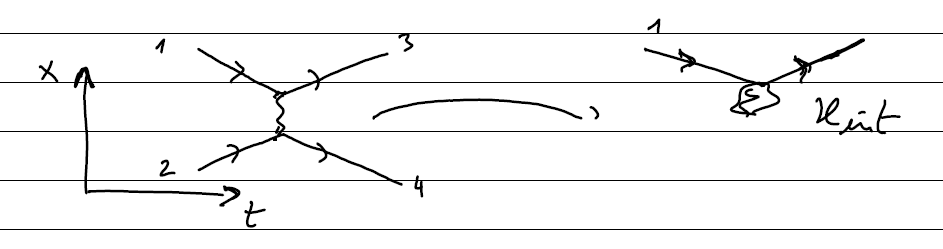
\includegraphics[scale=0.80]{Images4/partie 4 - interaction.PNG}
    \caption{Diagrammes de feynmann}
    \label{fig:feynmann_diagram}
\end{figure}



\subsection{Calcul explicite de la section efficace}


Nous allons maintenant expliciter $\lambda_{fi}$, le taux de transition par unité de temps de l'état $i$ vers l'état f. Pour rappel, nos hypothèses sont la collision élastique et l'absence de recul de la particule cible. La règle d'or de Fermi implique que:
\[
    \lambda_{fi} 
    \eq
    \dfrac{2\pi}{\hbar }|\mel{\psi_f}{t_{fi}}{\psi_i}|^2 \fdif{n_f}{E}
    \eq
    \dfrac{2\pi}{\hbar }|T_{fi}|^2 \fdif{n_f}{E}
\]

\subsubsection{Calcul de l'élément de matrice $T_{fi}$}\label{calcul_Tfi}

\[
    T_{fi} 
    \; \equiv \;
    \mel{\psi_f}{T_{fi}}{\psi_i}
    \eq
    \int \psi_f^* \cdot H_\text{int} \cdot \psi_i \quad \dif^3\vec{r}
\]
Plusieurs commentaires peuvent déjà se faire:
\begin{itemize}

    \item $T_{fi}$ peut être vu comme la somme des amplitudes qui, à partir d'un certain état initial de la particule $\alpha$ (ici, l'impulsion $\vec{P}_1$) donnent un certain état final (ici, l'impulsion $\vec{P}_3$) de cette même particule $\alpha$. On ne prend ainsi pas en compte la particule cible dans notre calcul : nous considérons l'absorption d'un \textbf{photon virtuel} (qui provient du noyau) par une particule $\alpha$. Ainsi, \textbf{la collision élastique avec le noyau est équivalente à l'absorption d'une photon virtuel}.
     
    Selon wikipédia\footnote{toi-mêm tu connais les bails \url{https://fr.wikipedia.org/wiki/Particule_virtuelle}}, le photon virtuel échangé ne viole apparemment pas la conservation de l'énergie grâce au principe d'incertitude. Comme la durée de l'interaction est très petite, il y a une grande incertitude sur l'énergie du photon virtuel. Sans le principe d'incertitude, il y aurait effectivement violation de la conservation de l'énergie.
    
    \item Le domaine d'intégration couvre tous les points où il peut y avoir une interaction entre la particule $\alpha$ et le noyau (pas l'atome ni son nuage électronique), c'est-à-dire où le potentiel est non-nul. Puisque l'interaction de la particule $\alpha$ avec le noyau est décrite par un potentiel coulombien, l'intégrale doit couvrir tout l'espace des positions. (Remarque : dans la réalité, il faut considérer le nuage électronique qui rend l'atome globalement neutre au-delà d'une certaine distance du noyau)
    
\end{itemize}
On peut maintenant remplacer les fonctions d'onde par leur expression impliquant uniquement l'impulsion (pour rappel les énergies se simplifient et ne sont donc pas notées). \textcolor{red}{supprimer footnote si le prof répond}\footnote{On a encore un problème ici : pourquoi ne pas considérer la quantité de mouvement du noyau si on simplifie les énergies? On pose que la qdm initiale du noyau est nulle car on se trouve dans sont référentiel ($p_2\;\equiv\;0$) mais on ne peut pas négliger sa qdm}
Nous rappelons aussi que la référentiel est celui du noyau  et que ce noyau a un recul nul ($p_4\;\approx\;0$)

Puisque nous ne nous intéressons qu'à la particule $\alpha$ avant et après la collision, nous n'avons pas besoin des fonctions d'onde\footnote{comme décrite à la section \ref{fct_onde}} initiale et finale de la particule cible (\textcolor{red}{QUESTION : Pourquoi pouvons-nous simplifier les énergies de l'expression alors? En effet, si nous ne prenons que les fonctions d'onde initiales et finales de la particule, on n'a pas la somme de toutes les énergies mais seulement de $E_1$ et $E_3$})
%alors pourquoi on pourrait simplifier les énergies si on ne considère pas toutes les fonctions d'onde ensemble? Doit-on quand même prendre ces fonction et leur imposer une qdm nulle?? Val : pour moi on doit considérer les fonction d'onde avant/après de la cible en les aprpoximant par des ondes planes et ensuite simplifier avec $p2 = 0$ (même si c'est un peu bizarre physiquement parlant) et $p_4 \approx 0$ en ignorant le recul)}. 
Nous pouvons également remplacer l'hamiltonien d'interaction $H_\text{int}$ par son expression. Nous obtenons ainsi :
\begin{align*}
    T_{fi}
&\eq
    \int \psi_f^* \cdot H_\text{int} \cdot \psi_i \quad \dif^3\vec{r}\\
&\eq
    \dfrac{1}{V} 
    \int 
    \exp(\dfrac{-\imag \vec{p_1}\cdot\vec{r}}{\hbar})     \cdot
    \exp(\dfrac{-\imag \vec{p_2}\cdot\vec{r}}{\hbar})     \cdot
    \dfrac{z_1 z_2\alpha\hbar c}{r}                     \cdot
    \exp(\dfrac{ \imag \vec{p_3}\cdot\vec{r}}{\hbar})     \cdot
    \exp(\dfrac{ \imag \vec{p_4}\cdot\vec{r}}{\hbar})
    \quad \dif^3\vec{r}\\
&\eq
    \dfrac{1}{V} 
    \int 
    \exp(\dfrac{-\imag \vec{p_3}\cdot\vec{r}}{\hbar})     \cdot
    \dfrac{z_1 z_2\alpha\hbar c}{|\vec{r}|}             \cdot
    \exp(\dfrac{ \imag \vec{p_1}\cdot\vec{r}}{\hbar})
    \quad \dif^3\vec{r}\\
\intertext{car $p_2\;\equiv\;0$ et $p_4\;\approx\;0$}
&\eq
    \dfrac{z_1 z_2\alpha\hbar c}{V} 
    \int 
    \dfrac{1}{|\vec{r}|} \cdot \exp(\dfrac{\imag \vec{q}\cdot\vec{r}}{\hbar})
    \quad \dif^3\vec{r} 
    \qquad \text{avec} \qquad \boxed{ \vec{q} \equiv \vec{p_1}-\vec{p_3}}
\end{align*}
Il faut maintenant résoudre l'intégrale. Étant donné qu'on évalue l'intégrand sur tout l'espace, on peut placer notre système d'axes comme on le souhaite. Ainsi, pour nous faciliter la vie, on choisit un système d'axes pour lequel $\vec{q}$ est dans l'axe $\hat{z}$ tel qu'en utilisant les coordonnées sphériques : $\vec{q}\cdot\vec{r} = (0,0,q)\cdot(0,0,r\cos{\beta}) = q\cdot r \cdot \cos(\beta)$ avec $\beta$ qui varie entre 0 et $\pi$. Pourquoi prendre $\beta$ au lieu $\theta$ vous demandez-vous en insultant l'auteur de ce déplorable choix. Simplement parce que $\theta$ est déjà réservé comme étant l'angle de diffusion entre $\vec{p}_1$ et $\vec{p_3}$ dans le système d'axes pour lequel $\vec{p_1} \parallel \hat{z}$ qui n'est donc pas le même que celui utilisé pour l'intégrale\footnote{Ça va la géométrie ?}. Cet angle $\theta$ est bien fixé puisque l'on s'intéresse ici au taux de transition entre état initial et un état final donné.
Ainsi, l'élément de volume infinitésimal s'écrit comme  $\dif^3\vec{r} = \dif r \cdot r \dif\beta \cdot r \sin(\beta) \dif\phi $ et l'intégrale devient :
\begin{align*}
    \int \dfrac{1}{r} \cdot \exp(\dfrac{\imag}{\hbar}\vec{q}\cdot\vec{r})
    \quad \dif^3\vec{r}
        &\eq
    \int_{0}^{2 \pi} \dif\phi
    \int_{0}^{+\infty} \dfrac{1}{r}r^2 
    \Bigg( 
        \int_{0}^{\pi}
        \exp(\dfrac{\imag qr}{\hbar}\cos(\beta)) \cdot \sin(\beta) \dif\beta
    \Bigg) \dif r\\
        &\eq
    2 \pi \cdot \int_{0}^{+\infty} r 
    \left[
      \dfrac{\hbar}{\imag qr}\exp(\dfrac{\imag qr}{\hbar}u)
    \right]^{1}_{-1}
    \dif r 
    \qquad \quad \text{via changement de var. } u = \cos(\beta)\\
        &\eq
    2 \pi \int_{0}^{+\infty} r
    \cdot \dfrac{2\hbar \sin(\dfrac{qr}{\hbar})}{qr} \dif r\\
        &\eq
    2 \pi \dfrac{2\hbar}{q} \int_{0}^{+\infty} \sin(\dfrac{qr}{\hbar}) \; \dif r\\
        &\eq
    \dfrac{4\pi\hbar^2}{q^2} \lim_{\epsilon \rightarrow 0}\int_{0}^{+\infty}\exp(-\epsilon \beta) \sin(\beta) \; \dif\beta\\
        &\eq
    \dfrac{4\pi\hbar^2}{q^2} \lim_{\epsilon \rightarrow 0}\dfrac{1}{1 + \epsilon^2}\\
        &\eq
    \dfrac{4\pi\hbar^2}{q^2}
    \qquad \quad \text{via un changement de var., une limite et 2 intégrales par partie\footnotemark} 
\end{align*}
\footnotetext{Il va sans dire qu'il s'agit d'une exercice trivial laissé à la sagacité de l'infortuné lecteur}
Par conséquent, l'élément de matrice $T_{fi}$, nécessaire pour obtenir l'expression du taux de transition, s'écrit:
\[
    T_{fi} 
    \eq 
    \dfrac{z_1 z_2\alpha\hbar c}{V} \cdot \dfrac{4 \pi \hbar^2}{q^2}
\]



\subsubsection{Détermination de densité d'états $\dif n_f/\dif E$}


Pour évaluer la densité d'états, on en revient aux principes de la physique statistique. Il s'agit d'évaluer le nombre de cellules élémentaires comprise dans un volume de l'espace des états. Le volume d'une cellule élémentaire de l'espace de $k$ est de $\dfrac{(2\pi)^3}{V}$ (Figure~\ref{fig:densite_etats}).
 \begin{figure}[htpb]
    \centering
    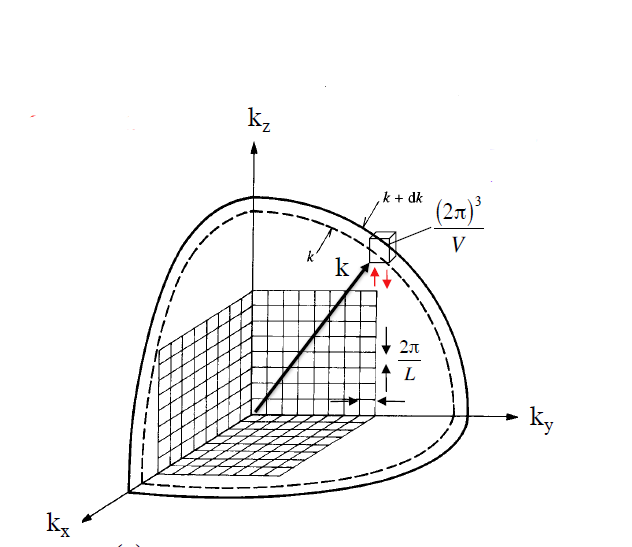
\includegraphics[scale=0.80]{Images4/dens.PNG}
    \caption{Schéma pour le calcul de la densité d'états}
    \label{fig:densite_etats}
\end{figure}
Supposons que l'on considère tous les vecteurs possédant une norme entre $P_f$ et $P_f + \dif P_f$ ($P_3 = P_f$). Nous pouvons alors écrire, pour le vecteur d'onde $k$ d'abord et ensuite pour la quantité de mouvement :
\begin{align*}
    \dif n_f 
        &\eq 
    \dfrac{\text{Volume coquille}}{\text{Volume élémentaire}}\\
        &\eq
    \dfrac{\text{Surface . incrément infinitésimal}}{\text{Volume élémentaire}}\\
        &\eq
    \dfrac{4\pi k^2 \cdot \dif k}{(2\pi)^3 / V}\\
        &\eq
    \dfrac{1}{\hbar^3}\dfrac{4\pi P^{2}_f \cdot \dif P_f}{(2\pi)^3 / V} 
    \qquad \quad \text{puisque} \quad
    \vec{P} \eq \hbar \cdot \vec{k} \qquad \text{(Longueur d'onde de De Broglie)}
\end{align*}
Cependant, dans notre problème, nous ne considérons qu'une section de ce cercle, correspondant à un angle infinitésimal $\dif\Omega$. Remarquant que $4\pi$ est l'angle solide d'une sphère entière, nous la remplaçons donc par $\dif\Omega$\footnote{Voilà le genre de rigueur qu'on obtient quand ce sont des ingénieurs qui font un document} : ceci nous permet de ne prendre que la fraction de cette sphère qui nous intéresse (= l'angle solide couvert par le détecteur). On obtient donc l'expression suivante pour la densité d'état finale : 
\[
    \dif n_f \eq \dfrac{1}{\hbar^3}\dfrac{P^{2}_f \cdot \dif P_f \cdot \dif\Omega}{(2\pi)^3 / V}
\]
 Cependant, dans l'expression de la règle d'or de Fermi, c'est $ \fdif{n_f}{E}$ qui apparaît. Par conséquent, nous devons nous pencher sur le terme $\dif E\equiv \dif E_0$ car nous définissons $E_0 = E_3 + E_4 = E_1 + E_2$ (collision élastique). La différentielle d'énergie est donc:
\begin{align*}
    \dif E_0 
        &\eq 
    \dif E_3 + \fdif{E_4}{P_4}\dif P_4\\
        &\eq
    \dif E_3 + \dfrac{c^2 P_4}{E_4}\dif P_4 
    \qquad \quad \text{car} \quad
    E_i^2 \eq P_i^2c^2 + M^2c^4
    \quad \Leftrightarrow \quad
    2E_i\dif E_i \eq 2c^2 P_i \dif P_i\\
        &\approx\;
    \dif E_3  \qquad \qquad \text{car} \quad v_4 \approx 0 \;\Rightarrow\; E_4 = m_2c^2 \;\Rightarrow\; \dfrac{c^2P_4}{E_4} \approx \dfrac{m_2c^2v_4^2}{m_2c^2} = v_4^2 \;\rightarrow\; 0
\end{align*}
Dès lors, la densité d'état par unité d'énergie (ce qu'on veut) est :
\begin{align*}
    \fdif{n_f}{E_0} \;\equiv\; \fdif{n_f}{E_f}
        &\eq
    \dfrac{1}{\hbar^3}\dfrac{ \dif\Omega \cdot P^{2}_f}{(2\pi)^3 / V} \fdif{P_f}{E_f}
    \eq
    \dfrac{V P_f^2}{(2\pi\hbar)^3} \fdif{P_f}{E_f} \dif\Omega
    \\
        &\eq
    \dfrac{V P_f^2}{(2\pi\hbar)^3} \dfrac{E_3}{c^2P_3} \dif\Omega
    \qquad \qquad \text{via} \quad E_3=E_f \quad \text{et formule d'Einstein développée au-dessus} \\ 
        &\eq
    \dfrac{V P_f^2}{(2\pi\hbar)^3}\dfrac{m_3 c^2}{c^2 m_3 v_3}  \dif\Omega
    \qquad \quad \text{car} \quad E_{\text{cinétique}} << E_{\text{masse}} \quad \text{(vérifié avec valeurs sur Wiki)}\\
        &\eq
    \dfrac{V P_f^2}{(2\pi\hbar)^3}\dfrac{1}{v_3}  \dif\Omega
\end{align*}


\begin{comment}
Notre premier sentiment serait de simplement ignorer la variation d'énergie de la cible ($E_4 = E_\text{cible} = cst$) et d'écrire simplement : $\dif E_0 = \dif E_3$ où $E_0 = E_3 + E_4 = E_1 + E_2$ (collision élastique).\\
Cependant cette approximation n'est pas vraiment satisfaisante et nous développons donc ainsi : 
\begin{align*}
    \dif E_0 
        &\eq 
    \dif E_3 + \fdif{E_4}{P_4}\dif P_4\\
        &\eq
    \dif E_3 + \dfrac{c^2 P_4}{E_4}\dif P_4 
    \qquad \quad \text{car} \quad
    E_i^2 \eq P_i^2c^2 + M^2c^4
    \quad \Leftrightarrow \quad
    2E_i\dif E_i \eq 2c^2 P_i \dif P_i
\end{align*}
Or, nous avons supposé que le recul de la particule cible était négligeable, c'est-à-dire que la vitesse de la particule cible après la collision est considérée nulle :\\
OUI MAIS SA QDM DOIT PAS ETRE NULLE CAR ON MULTIPLIE PAR SA MASSE QUI EST INFINIE...ON DOIT DONC OBTENIR UN RESULTAT FINI NON-NUL POUR SA QDM
\[
    v_4 \rightarrow 0
        \quad \Leftrightarrow\quad
    P_4 \rightarrow 0
        \quad \Leftrightarrow\quad
    \dif E_0 \approx \dif E_3
        \quad \text{en l'absence de recul de la cible}
\]
\end{comment}





\subsubsection{Expression de $\lambda_{fi}$}


Nous avons donc obtenu l'élément de matrice $T_{fi}$ et la densité d'états finaux $ \fdif{n_f}{E_f}$. Nous avons donc $\lambda_{fi}^\text{exp}$ le taux de \textit{détection} dans un angle solide $\dif\Omega$ grâce à l'équation \eqref{lambda_exp} et $\lambda_{fi}$ le taux de \textit{transition} d'un état $i$ vers un continuum d'états $f$ situés dans un angle solide $\dif\Omega$ grâce à la règle d'or de Fermi. Nous réécrivons ces deux taux :

\[
    \left\{
    \begin{array}{ll}
        \lambda_{fi} \eq
        \dfrac{2\pi}{\hbar} |T_{fi}|^2 \fdif{n_f}{E}
        \eq
        \dfrac{2\pi}{\hbar} 
        \left(
            \dfrac{z_1 z_2\alpha\hbar c}{V} \cdot \dfrac{4 \pi \hbar^2}{q^2}  
        \right)^2
        \left(
        \dfrac{V P_f^2}{(2\pi\hbar)^3}\dfrac{1}{v_3}  \dif\Omega
        \right)
    \\[13pt]
        \lambda_{fi}^\text{exp} 
            \; \equiv \;
        \dfrac{N_\text{inc}}{V} v_1 \fdif{\sigma}{\Omega} \dif\Omega
            \eq
        \dfrac{1}{V} v_1
        \fdif{\sigma}{\Omega} \dif\Omega \qquad \qquad \text{En normalisant à une particule par unité de volume}
    \end{array}
    \right.
\]
Si l'on considère que le détecteur est parfait (efficacité de 100\% : il détecte toutes les particules qui l'atteignent), on peut égaliser ces deux taux en les associant au même angle solide $\dif\Omega$. Ainsi, on peut obtenir l'expression de la section efficace différentielle $\fdif{\sigma}{\Omega}$. Il est à noter que le terme $I = \dfrac{v_1}{V} \left[\dfrac{\# \alpha}{\si{m^2\cdot s}}\right]$ est l'intensité normalisée ($N_\text{inc} = 1$):

\[
    \fdif{\sigma}{\Omega}
        \eq
    \lambda_{fi} \cdot \dfrac{V}{v_1 \dif\Omega}
        \; \equiv \;
    \dfrac{ \lambda_{fi}}{I \dif\Omega}
        \eq
    \dfrac{2\pi}{\hbar} 
    \left(
        \dfrac{z_1 z_2\alpha\hbar c}{V} \cdot \dfrac{4 \pi \hbar^2}{q^2}  
    \right)^2
    \left(
    \dfrac{V P_f^2}{(2\pi\hbar)^3}\dfrac{1}{v_3}  \dif\Omega
    \right)
    \cdot
    \dfrac{V}{v_1 \dif\Omega}
        \eq
    4 \left( \dfrac{z_1 z_2e^2}{4\pi\epsilon_0} \right)^2 \dfrac{P_f^2}{q^4v_1v_3}
\]
Ce résultat ne dépend pas donc pas du volume $V$ ni de $\hbar$ ($\alpha \hbar$ est indépendant de $\hbar$) : le résultat est donc valable en physique classique (lorsque $\hbar \rightarrow 0$).
Cette dernière expression de la section efficace différentielle peut se simplifier. On peut en effet ré-exprimer $q^4$ avec $P_f \equiv |\vec{P}_f|$ :

\begin{align*}
    \vec{q} \eq \vec{P}_1 - \vec{P}_3
        &\quad \Leftrightarrow \quad
    q^2 \eq P_1^2 + P_3^2 - 2 \cdot \vec{P}_1 \cdot \vec{P}_3\\
        &\quad \Leftrightarrow \quad
    q^2 \eq 2 P_f^2 - 2 P_f^2 \cos(\theta)
    \qquad \text{collision élastique sans recul} \quad \Leftrightarrow \quad v_1=v_3\\
        &\quad \Leftrightarrow \quad
    q^2 \eq 4 P_f^2 \sin^2\left(\dfrac{\theta}{2}\right)
\end{align*}
En injectant ce résultat dans l'expression de  $\dfrac{\dif\sigma}{\dif\Omega}$ :
\begin{align*}
    \fdif{\sigma}{\Omega}
        &\eq
    \Bigg( \dfrac{z_1 z_2e^2}{4\pi\epsilon_0} \Bigg)^2 
    \dfrac{4 P_f^2}{16 P_f^4 \sin^4\left(\dfrac{\theta}{2}\right)v^2_1}\\
        &\eq
    \Bigg( \dfrac{z_1 z_2e^2}{4\pi\epsilon_0} \Bigg)^2
    \dfrac{1}{ \left(\dfrac{P_1v_1}{2}\right)^2 16\sin^4\left(\dfrac{\theta}{2}\right)}
    \qquad \text{Il apparaît l'énergie cinétique de la particule incidente}\\
    &\eq
    \Bigg( \dfrac{cst}{E_\text{cin}} \Bigg)^2
    \dfrac{1}{16\sin^4\left(\dfrac{\theta}{2}\right)}
\end{align*}
Ce dernier résultat est exactement le même que le résultat obtenu classiquement. La règle d'or de Fermi nous a donc permis de retrouver l'expression classique de la section efficace de Rutherford. On peut ainsi, sans l'avoir démontrée par la théorie des perturbation, accepter la validité de la règle d'or de Fermi.






\section{Détermination de la densité de charge du noyau}
\subsection{Introduction et motivations}

Nous savons grâce à l'expérience de Rutherford et au calcul de la section efficace qu'il existe des centres diffuseurs au sein d'un matériau. Ces centres diffuseurs sont les noyaux des atomes. Nous nous intéressons maintenant à la taille et à la structure interne de ces noyaux : Sont-ils ponctuels? De quoi sont-ils composés?

Imaginons que nous voulions sonder la structure interne des centres diffuseur avec des électrons. Nous allons ainsi étudier la \textbf{diffusion élastique} des électrons par le noyau : $e^- + \text{noyau} \rightarrow e^- + \text{noyau}$
Nous savons qu'un noyau a une taille de l'ordre de quelques femtomètres\footnote{On avait ASKIP vu que la particule $\alpha$ pouvait se rapprocher jusqu'à quelques dizaines de femtomètres du centre diffuseur}. Par conséquent, si nous voulons sonder ces échelles avec des électrons, quelle doit être leur énergie? Pour pouvoir sonder un objet, la particule doit avoir une longueur d'onde de de Broglie de l'ordre de la taille de cet objet. Pour un noyau ayant une taille de 2 femtomètres:

\begin{equation}
    \lambda_e \eq \dfrac{h}{p} \eq \SI{2}{fm}
    \quad \Leftrightarrow \quad
    E_e \stackrel{\text{ultra-rel}}{\approx}c\cdot p \eq \dfrac{hc}{\lambda_e} 
    \; \approx \;
    \SI{600}{MeV}
\end{equation}
Les électrons devant sonder des noyaux ayant une taille de l'ordre de 2 femtomètres doivent avoir des énergies de 600 [{MeV}]. La masse de l'électron étant de \SI{0.5}{MeV}, nous nous trouvons donc dans un cas ultra-relativiste (car E$_\text{cin}$ $>>$ E$_\text{masse}$).


\subsection{Cas d'un noyau ponctuel}


Nous allons ici étudier la collision élastique d'un électron avec un noyaux ponctuel en négligeant le recul du noyau (M$_\text{noyau}\approx Z \cdot 1800 \cdot$ m$_e$ $>>$ m$_e$). En reprenant le résultat de la collision élastique de particules $\alpha$ avec des noyaux ponctuels sans recul, nous obtenons dans notre cas, pour une jauge $\hbar=c=1$:

\[
    \left(  \fdif{\sigma}{\Omega} \right)_\text{Ruth}^\text{el}
    \eq
    4 \left( \dfrac{z_1 z_2e^2}{4\pi\epsilon_0} \right)^2 \dfrac{P_f^2}{q^4v_1v_3}
    \eq
    \dfrac{4 (z_1 z_2 \alpha)^2 P_f^2}{q^4v_1v_3}
\]
Nous pouvons simplifier l'expression du dessus avec:

\begin{itemize}

    \item Puisque l'énergie de masse des électrons est négligeable devant leur énergie cinétique, nous pouvons considérer ces électrons comme ultra-relativistes, c'est-à-dire pour lesquels $v_1=v_3=c=1$. Dès lors,
    \[
        E^2 \;\approx\; P^2c^2 \eq P^2
    \]
    
    \item En utilisant l'hypothèse de collision élastique sans recul de la cible, nous avons:
    \begin{align*}
        \vec{q} \eq \vec{P}_1 - \vec{P}_3
            &\quad \Leftrightarrow \quad
        q^2 \eq P_1^2 + P_3^2 - 2 \cdot \vec{P}_1 \cdot \vec{P}_3\\
            &\quad \Leftrightarrow \quad
        q^2 \eq 2 P_f^2 - 2 P_f^2 \cos(\theta)
        \qquad \text{collision élastique sans recul : } v_1=v_3\\
            &\quad \Leftrightarrow \quad
        q^2 \eq 4 P_f^2 \sin^2\left(\dfrac{\theta}{2}\right)\\
            &\quad \Leftrightarrow \quad
        q^2 \eq 4 E^2   \sin^2\left(\dfrac{\theta}{2}\right)
    \end{align*}
\end{itemize}
Avec ces deux informations, la section efficace différentielle devient :
\[
    \left(  \fdif{\sigma}{\Omega}  \right)^\text{el}_\text{Ruth}
    \eq
    \dfrac{4 (z_1 z_2 \alpha)^2 P_f^2}{q^4v_1v_3}
    \eq
    \dfrac{4 (z_1 z_2 \alpha)^2 E^2}{q^4}
    \eq
    \dfrac{4 (z_1 z_2 \alpha)^2 E^2}{16 E^4 \sin^4\left(\dfrac{\theta}{2}\right)}
    \eq
    \dfrac{(z_1 z_2 \alpha)^2}{4E^2}
    \dfrac{1}{\sin^4\left(\dfrac{\theta}{2}\right)}
\]
En se rappelant que nous travaillons avec un faisceau d'électrons ($z_2 = 1$) et en notant Z la charge du noyau : 
\begin{equation}
    \left(  \fdif{\sigma}{\Omega}  \right)^\text{el}_\text{Ruth}
    \eq
    \dfrac{Z^2}{4}\dfrac{\alpha^2}{E^2}\dfrac{1}{\sin^4(\theta/2)}
    \label{sect_eff_ponct}
\end{equation}
L'expression \ref{sect_eff_ponct} décrit, pour rappel, la section efficace différentielle de Rutherford dans le cas d'une diffusion élastique sans recul d'électrons ultra-relativistes par un noyau ponctuel. Regardons maintenant ce que vaut cette section de Rutherford dans le cas d'un noyau non-ponctuel.


\subsection{Cas d'un noyau non-ponctuel}\label{sec:noyau_non_ponctuel}


Si maintenant le noyau n'est plus ponctuel, nous devons modifier nos calculs. Nous supposons cependant que ce noyau a une symétrie sphérique (la densité de charge n'est fonction que du rayon par rapport au centre : $\rho_\text{ch} = \rho_\text{ch}(\vec{R}) = \rho_\text{ch}(R)$. En outre, on peut normaliser cette distribution de charge : $\rho_\text{ch} = ze\cdot \rho(R)$ tel que l'intégrale de $\rho(R)$ sur tout l'espace des $R$ soit égale à 1 ($ze$ est la charge totale du noyau).

L'interaction se fait comme suivant : l'onde plane (état non-lié $\Rightarrow$ continuum d'énergie) interagit en un point donné avec le noyau. Cette interaction se fait via le potentiel d'interaction H$_\text{int}$ (énergie du photon virtuel émis) qui dépend de la position d'un point d'interaction par rapport au centre de la sphère. Si ce point est situé loin du noyau, on doit retomber sur l'interaction dans le cas du modèle ponctuel du noyau.

\begin{figure}[htpb]
    \centering
    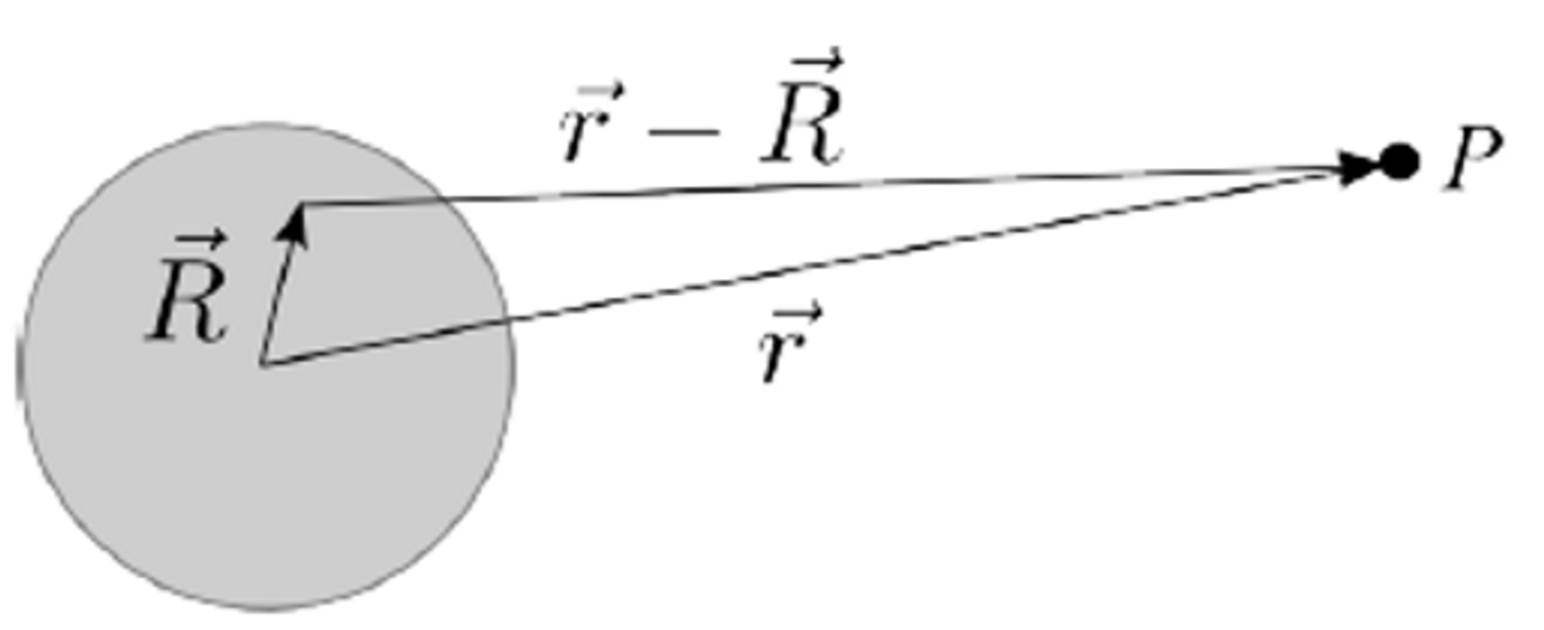
\includegraphics[scale=0.2]{Images4/schema_interaction.png}
    \caption{$P$ est la particule qui interagit avec le noyau. $\vec{R}$ est le vecteur position de l'élément de volume nucléaire chargé dans le noyau. $\vec{r}$ est le vecteur position du point auquel on considère le potentiel. $\vec{r}-\vec{R}$ est la distance entre la particule incidente et l'élément de volume chargé du noyau.}
    \label{fig:schema_interaction}
\end{figure}

Les vecteurs reliant le centre du noyau au détecteur et le point d'interaction entre l'électron et le noyau au détecteur peuvent être considérés parallèles si le détecteur est placé à grande distance (ce qui est le cas ; approximation de Fraunhofer). Sur le Figure~\ref{fig:schema_interaction} on peut voir que le vecteur reliant le centre diffuseur dans le noyau au point d'observation est $\vec{r} - \vec{R}$.

Cette distribution de charge ne va modifier que le terme $T_{fi}$ (donc $\lambda_{fi}$) au travers de $H_\text{int}$:

\[
    H_\text{int} \eq \dfrac{z_1z_2e^2}{4\pi\epsilon_0} \int \dfrac{\rho(\vec{R})}{|\vec{r} - \vec{R}|} \quad \dif^3\vec{R}
\] 
On applique ici les préceptes de la mécanique quantique : la probabilité est le carré de la somme des amplitudes (et non la somme des carrés des amplitudes, qui est la somme des probabilités). Dès lors, on additionne les probabilités sur tous les vecteurs $\vec{R}$ auxquels peut se faire l'interaction, d'où l'intégrale sur $\vec{R}$, qui a pour domaine l'ensemble de l'espace. En injectant cette expression dans l'élément de matrice $T_{fi}$ : \textcolor{red}{Encore une fois on prend juste les fonctions d'onde de seulement d'électron sans compter l'énergie, ce qui pose problème...c'est la même question qu'avant.}
\begin{align*}
    T_{fi} 
&\; \equiv \;
    \int \phi^*_{e'} \cdot H_\text{int} \cdot \phi_e \quad \dif^3\vec{r}\\
&\eq 
    \int 
    e^{-\imag\vec{P'} \cdot\vec{r}}
    \Bigg(
        \dfrac{z_1z_2e^2}{4\pi\epsilon_0} \int \dfrac{\rho(\vec{R})}{|\vec{r} - \vec{R}|} \quad \dif^3\vec{R}
    \Bigg)
    e^{\imag\vec{P} \cdot\vec{r}}
    \quad \dif^3\vec{r}\\[4pt]
& \eq 
    \dfrac{z_1z_2e^2}{4\pi\epsilon_0} \int 
    e^{\imag\vec{q} \cdot\vec{r}}
    \Bigg(
         \int \dfrac{\rho(\vec{R})}{|\vec{r} - \vec{R}|} \quad \dif^3\vec{R}
    \Bigg)
    \quad \dif^3\vec{r}
    \qquad \qquad \;\; \text{avec} \quad \vec{q} \eq \vec{P}-\vec{P'}
    \\[4pt]
& \eq 
    \dfrac{z_1z_2e^2}{4\pi\epsilon_0} \int 
    \rho(\vec{R}) \cdot e^{\imag\vec{q} \cdot\vec{R}}
    \Bigg(
         \int \dfrac{ e^{\imag\vec{q} \cdot\vec{s}}   }{|\vec{s}|} \quad \dif^3\vec{s}
    \Bigg)
    \quad \dif^3\vec{R}
    \qquad \quad \text{avec} \quad \vec{s} = \vec{r}-\vec{R} \; \Leftrightarrow \; \dif s_x = \dif(r_x - R_x) = \dif r_x
    \\[4pt]
& \eq 
    \dfrac{z_1z_2e^2}{4\pi\epsilon_0} \int 
    \rho(\vec{R}) \cdot e^{\imag\vec{q} \cdot\vec{R}}
    \cdot \left( \dfrac{4\pi(\hbar = 1)^2}{q^2} \right)
    \quad \dif^3\vec{R}
    \qquad \quad \;\; \text{intégrale déjà résolue à la section \eqref{calcul_Tfi}}
    \\[4pt]
& \eq 
    \dfrac{z_1z_2e^2}{4\pi\epsilon_0} \dfrac{4\pi}{q^2} \cdot
    \Bigg(
    \int 
    \rho(\vec{R}) \cdot e^{\imag\vec{q} \cdot\vec{R}}
    \quad \dif^3\vec{R}
    \Bigg)
    \qquad \qquad \qquad \quad \text{ici  }  z_1 = -1; z_2 = Z_\text{cible}
    \\[4pt]
& \eq 
    \dfrac{-Z_\text{cible}e^2}{4\pi\epsilon_0} \dfrac{4\pi}{q^2}
    \cdot F(\vec{q})
    \eq
    (T_{fi})^\text{ponctuel} \cdot F(\vec{q})
    \\
\end{align*}
On observe ainsi que, dans le cas d'un noyau non-ponctuel, l'élément de matrice $T_{fi}$ est égal à l'élément $T_{fi}$ dans le cas d'un noyau ponctuel multiplié par un facteur correctif $F(\vec{q})$ lié à la non-ponctualité du noyau. Ce facteur correctif est fonction de la densité de charge $\rho$ et du changement de $\vec{q}$, la quantité de mouvement du photon de l'échange. On peut citer deux propriétés intéressantes du facteur de forme:
\begin{itemize}
    \item Si l'électron n'est pas diffusé par le noyau, alors $\vec{q}=\vec{0}$ :
          \[
            F(\vec{q}=0) \eq 
            \int \rho(\vec{R}) \cdot e^{\imag\cdot0} \; \dif^3\vec{R} \eq
            \int \rho(\vec{R}) \; \dif^3\vec{R} \;\equiv\; 1
          \]
          
    \item Si la distribution de charge est ponctuelle (i.e. $\rho(\vec{R})= \delta(\vec{R})$), alors le facteur de forme est unitaire:
    \[
        F_{pt}(\vec{q}) \eq 
        \int \delta(\vec{R}) \cdot e^{\imag\vec{q} \cdot\vec{R}} \; \dif^3\vec{R} \eq
        \int \delta(\vec{R}) \; \dif^3\vec{R} \;\equiv\; 1
    \]
    Ainsi, si le noyau est ponctuel (densité de charge est un delta de Dirac), on retombe bien sur l'expression de la section efficace ponctuelle.
\end{itemize}
En fait, le facteur $F(\vec{q})$, appelé plus communément \textbf{facteur de forme}, est \textbf{la transformée de Fourier de la distribution de charges}. On obtient donc $\rho(\vec{R})$ en mesurant $F(\vec{q})$ et en appliquant au résultat la transformée de Fourier inverse. Pour mesurer $F(\vec{q})$, il suffit de connaître la section efficace de Rutherford (c'est-à-dire la section efficace pour un noyau ponctuel avec une interaction sans recul) et de la comparer à une mesure expérimentale de la section efficace. Il faut cependant rester prudent avec le résultat obtenu : un résultat plus précis sera obtenu en utilisant un recul de la particule cible (qui aurait donc une masse finie).\\

Nous étudions donc la collision élastique d'un électron ponctuel avec une particule cible non-ponctuelle, caractérisée pas une densité de charge et supposée de masse infinie (pas de recul). Avec nos résultats, nous pouvons maintenant étudier la section efficace différentielle de cette diffusion : il s'agit de la même section efficace différentielle que dans le cas ponctuel, avec cependant la correction $|F(\vec{q})|^2$ due au caractère non-ponctuel du noyau:
\[
    \left( \fdif{\sigma}{\Omega} \right)^\text{exp}
    \eq
    \left( \fdif{\sigma}{\Omega} \right)^\text{Ruth}
    \cdot |F(\vec{q})|^2
    \qquad \quad \text{avec} \quad
    F(\vec{q}) \eq \int 
    \rho(\vec{R}) \cdot e^{\imag\vec{q} \cdot\vec{R}}
    \quad \dif^3\vec{R}
\]
Il est cependant possible d'obtenir un résultat plus précis en considérant un recul de la particule cible (donc noyau de masse finie), c'est-à-dire que l'énergie de l'électron sera moindre après la collision (énergie après = $E'<E$ = énergie avant). Ainsi, si on veut tenir compte de la masse du noyau, il faut modifier l'expression de $\fdif{P_f}{E_f}$ :
\[
    \fdif{P_f}{E_f} \;\approx\; \dfrac{P'}{cP} \eq \dfrac{E'}{cE}
    \qquad \text{avec $c$ la vitesse de l'électron (ultra-relativiste)}
\]
Par conséquent, la section efficace pour un noyau ponctuel de masse finie (donc collision élastique avec recul) est mieux décrite par la formule suivante (qu'on démontrera apparemment en TP) :
\[
    \left( \fdif{\sigma}{\Omega} \right)^\text{ponctuel}
    \eq
    \left( \fdif{\sigma}{\Omega} \right)^\text{Ruth}
    \cdot \dfrac{E'}{E}
    \qquad \text{avec} \quad
    \dfrac{E'}{E} \eq
    \dfrac{1}{1+\dfrac{E}{M}(1-\cos(\theta))} 
    \quad \text{tq $M$ est la masse du noyau} \quad 
\]
En utilisant ce résultat pour décrire la section efficace de la diffusion d'un électron par un noyau non-ponctuel en tenant compte du recul du noyau :
\[
\boxed{
    \left( \fdif{\sigma}{\Omega} \right)^\text{elec}
    \eq
    \left( \fdif{\sigma}{\Omega} \right)^\text{Ruth}
    \cdot \dfrac{E'}{E}
    \cdot |F(\vec{q})|^2
    \qquad \text{avec} \quad 
     F(\vec{q}) = \int 
    \rho(\vec{R}) \cdot e^{\imag\vec{q} \cdot\vec{R}}
    \; \dif^3\vec{R}
    \quad \text{et} \quad
    \vec{q} = \vec{P}_e - \vec{P'}_e
}
\]
Comme dit précédemment, on sait que ce facteur de forme $F(\vec{q})$ représente la transformée de Fourier de la densité de charge du noyau. Alors qu'il nous est impossible de mesurer la densité de charge, nous pouvons mesurer le facteur de forme. Il suffit ensuite de prendre la transformée de Fourier inverse de la mesure de $F(\vec{q})$ pour obtenir la densité de charge.\\
De façon plus pragmatique, nous mesurons la section efficace pour notre diffusion que nous pouvons relier à $|F(\vec{q})|^2$:
\[
    |F(\vec{q})|^2 \eq
    \left( \fdif{\sigma}{\Omega} \right)^\text{elec}
    \cdot
    \Bigg[
    \left( \fdif{\sigma}{\Omega} \right)^\text{Ruth}
    \cdot \dfrac{E'}{E}
    \Bigg]^{-1}
\]
\begin{figure}[H]
    \centering
    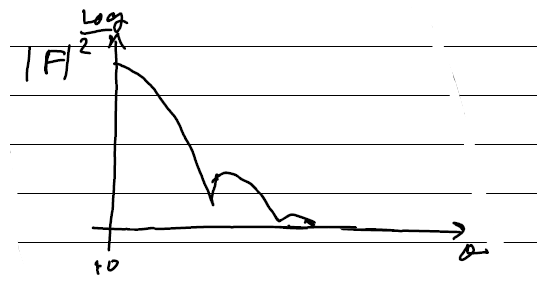
\includegraphics[scale=0.80]{Images4/graphe 2.PNG}
    \caption{Facteur de forme extrait de la section efficace expérimentale en fonction de l'angle de détection}
    \label{fig:Facteur de forme expériemental}
\end{figure}
On observe ainsi que la figure \eqref{fig:Facteur de forme expériemental} est similaire à la diffraction provoquée par un disque (un trou circulaire, une sphère). Aurait-on donc trouvé la forme de notre noyau? Exactement! Mais pour prouver cela, nous allons d'abord nous intéresser à d'autres formes de noyau, telles que le cube.\footnote{Franchement le mec qui a pensé à ça il était pas carré MDR (j'ai aussi la même avec `quelque chose tournait pas rond chez lui' si vous voulez)}



\subsubsection{Densité de charge cubique}

Dans l'élaboration d'une théorie, on passe souvent par des modèles très simples, qui nous permettent d'appréhender les phénomènes physiques sans trop nous buter en algèbre. Pour ce qui est de notre noyau, nous allons, avant même de considérer un noyau avec une épaisseur, considérer un noyau carré (plan). Ainsi, la densité de charge dans ce modèle est constante sur le carré et nulle ailleurs :
\[
    \rho(\vec{R}) \eq
    \left\{
    \begin{array}{ll}
        \dfrac{1}{\Delta x} \dfrac{1}{\Delta y} \delta(z)
        \overset{\text{norm.}}= 
        \dfrac{1}{D}\dfrac{1}{D}\delta(z)
        \qquad \text{si} \quad
        x,y \;\in\; \big[ -\dfrac{D}{2},\dfrac{D}{2} \big] \\[7pt]
        0 \qquad \qquad \qquad \qquad \qquad \qquad \quad \text{sinon}
    \end{array}
    \right.
\]
On vérifie bien avec une telle densité de charge (normalisée) que son intégrale sur tout le domaine est effectivement égale à 1: (Voir Figure~\ref{fig:densite_carree})
\[
    \int \rho(\vec{R}) \dif^3\vec{R}
    \eq
    \int_{-D/2}^{D/2}\dfrac{1}{D} \dif x
    \int_{-D/2}^{D/2}\dfrac{1}{D} \dif y
    \int_{-\infty}^{\infty}\delta (z)\dif z
    \eq 1\cdot 1 \cdot 1
\]
\begin{figure}[H]
    \centering
    \includegraphics[scale=0.40]{Images4/Densite_carrée.png}
    \caption{Illustration de la densité de charge carrée}
    \label{fig:densite_carree}
\end{figure}
La densité de charge étant maintenant connue, nous pouvons calculer sa transformée de Fourier afin d'obtenir $F(\vec{q})$. Pour ce faire, nous allons considérer que l'électron incident sur ce noyau carré a une quantité de mouvement alignée avec l'axe $z$. En ce qui concerne la quantité de mouvement de l'électron diffusé, elle n'a pas d'orientation précise. Ainsi, $\vec{q} \equiv \vec{P}-\vec{P'} = (0,0,P)-(P'_x,P'_y,P'_z) = (-P'_x,-P'_y,P-P'_z) $. On tient également à rappeler que la TF d'une fonction créneau est un sinus cardinal et que la TF d'un delta de Dirac est 1.
Nous pouvons ainsi écrire $F(\vec{q})$:
\begin{align*}
    F(\vec{q}) 
    &\eq
    \int \rho(\vec{R}) \cdot e^{\imag\vec{q} \cdot\vec{R}} \quad \dif^3\vec{R}\\
    &\eq
    \int \rho(x,y,z) \cdot \exp[\imag(-P'_x,-P'_y,P-P'_z) \cdot(x,y,z)] \quad \dif x\dif y\dif z\\
    &\eq
    \int_{-D/2}^{D/2}\dfrac{1}{D}     \cdot \exp(-\imag P'_xx) \dif x
    \int_{-D/2}^{D/2}\dfrac{1}{D}     \cdot \exp(-\imag P'_yy) \dif y
    \int_{-\infty}^{\infty} \delta(z) \cdot \exp(\imag (P-P'_z)z) \dif z\\
    &\eq
    \sinc\left(\dfrac{P'_xD}{2}\right) \cdot
    \sinc\left(\dfrac{P'_yD}{2}\right) \cdot 1\\
    &\eq
    \sinc\left(\dfrac{P \sin(\theta)\cos(\phi)D}{2}\right) \cdot
    \sinc\left(\dfrac{P \sin(\theta)\sin(\phi)D}{2}\right)
    \qquad \text{si} \quad |\vec{P'}|\eq|\vec{P}| \quad \text{(pas de recul)}
\end{align*}
Nous nous intéressons aux zéros de cette fonction : sous quel angle d'observation n'observe-t-on aucun électron? Plus pragmatiquement, nous nous intéresserons surtout au premier zéro de $F(\vec{q})$ : en effet, puisqu'il s'agit d'une figure de diffraction, le premier zéro nous indiquera la dimension de l'objet. Notre détecteur va sonder tous les angles possibles (donc tous les couples $(\phi,\theta)$) ; intéressons-nous donc aux cas extrêmes de ces angles : 
\begin{itemize}
    
    \item Pour $\phi=0$ (ou de façon équivalente, $\phi=0,\dfrac{\pi}{2},\pi,\dfrac{3\pi}{2},...$), $F(\vec{q})$ vaut:
    \[
        F(\vec{q})  \eq \sinc\left(\dfrac{P \sin(\theta)\cdot 1 \cdot D}{2}\right)\cdot \sinc(0) 
        \eq \sinc\left(P\dfrac{\sin(\theta)D}{2}\right)
        \eq \sinc\left(\dfrac{2\pi}{\lambda}\dfrac{\sin(\theta)D}{2}\right)
    \]
    Où l'on a utilisé la longueur d'onde de De Broglie $\lambda = \dfrac{h}{p} = \dfrac{\hbar(=1) 2\pi}{p} = \dfrac{2\pi}{p}$. Souhaitant étudier les zéros de cette fonction, nous regardons les valeurs pour lesquelles l'argument du sinc vaut $\pi$:
    \[
        \pi 
        \eq \dfrac{2\pi}{\lambda}\dfrac{\sin(\theta)D}{2}
        \quad \Leftrightarrow \quad
        \sin(\theta) \eq \dfrac{\lambda}{D}
    \]
    
    \item Pour $\phi=\pi/4$ (ou de façon équivalente, $\phi=\dfrac{\pi}{4},\dfrac{3\pi}{4},\dfrac{5\pi}{4},...$), on a que $\cos(\phi)=\sin(\phi)=\dfrac{1}{\sqrt{2}}$. Par conséquent, $F(\vec{q})$ vaut:
    \[
        F(\vec{q})  \eq 
        \sinc\left(\dfrac{P \sin(\theta)\cdot 1 \cdot D}{2\sqrt{2}}\right)
        \cdot 
        \sinc\left(\dfrac{P \sin(\theta)\cdot 1 \cdot D}{2\sqrt{2}}\right)
        \eq \sinc^2 \left(P \dfrac{\sin(\theta)D}{2\sqrt{2}}\right)
        \eq \sinc^2 \left(\dfrac{2\pi}{\lambda}\dfrac{\sin(\theta)D}{2\sqrt{2}}\right)
    \]
    Souhaitant étudier les zéros de cette fonction, nous regardons les valeurs pour lesquelles l'argument du sinc vaut $\pi$:
    \[
        \pi 
        \eq \dfrac{2\pi}{\lambda}\dfrac{\sin(\theta)D}{2\sqrt{2}}
        \quad \Leftrightarrow \quad
        \sin(\theta) \eq \sqrt{2}\dfrac{\lambda}{D} \;\approx\; 1,4\dfrac{\lambda}{D}
    \]
\end{itemize}
Nous pouvons faire deux remarques quant à la modélisation de la densité de charge par une densité constante sur un carré (plan) et nulle ailleurs.


    \subsubsection{Critique de notre modèle carré : épaisseur du noyau}


Notre modèle considère un carré plan. Ne devrions-nous pas plutôt le doter d'une épaisseur? Nous aurions donc comme densité de charge $\rho(\vec{R}) = \dfrac{1}{\Delta x}\dfrac{1}{\Delta y} \dfrac{1}{\Delta z} \overset{\text{norm.}}= \dfrac{1}{D}\dfrac{1}{D} \dfrac{1}{D}$. Ainsi, remplacer $\delta(z)$ par $1/D$ revient multiplier l'expression de $F(\vec{q})$ par la transformée de Fourier de cette fonction créneau:
\[
    TF\left[ \dfrac{1}{D} \right] \eq
    \int_{-D/2}^{D/2}\dfrac{1}{D} \cdot e^{-i(P-P'_z)z} \dif z
    \eq
    \sinc\left(\dfrac{(P - P \cos(\theta))D}{2}\right)
    \eq
    \sinc\left(\dfrac{2\pi}{\lambda} \dfrac{D}{2} 
    \big[ 1-\cos(\theta) \big]\right)
\]
On obtient cette expression car selon l'axe z on a : $P - P'_z = P\left(1 - \cos(\theta) \right)$. Ainsi, en insérant une épaisseur dans le carré, $F(\vec{q})$ vaut:
\[
    F(\vec{q}) \eq 
    \sinc\left(\dfrac{P \sin(\theta)\cos(\phi)D}{2}\right) \cdot
    \sinc\left(\dfrac{P \sin(\theta)\sin(\phi)D}{2}\right) \cdot
    \sinc\left(\dfrac{2\pi}{\lambda} \dfrac{D}{2} 
    \big[ 1-\cos(\theta) \big]\right)
\]
Nous voulons maintenant savoir quels sont les minima induits pas le sinus cardinal ajouté par l'épaisseur du noyau carré, et plus particulièrement connaître la position du premier minima. Encore une fois, pour que le sinc lié à l'orientation $z$ soit nul, son argument doit être égal à $\pi$.
A partir de la relation trigonométrique $1-\cos(\theta) = 2\sin^2(\theta /2)$, nous pouvons écrire:
\[
    \pi \eq
    \dfrac{2\pi}{\lambda} \dfrac{D}{2}
    2 \sin^2(\theta /2)
    \quad \Leftrightarrow \quad
    \sin^2(\theta /2) \eq \dfrac{\lambda}{2D}
\]
Et pour de petits angles, $\sin^2(\theta /2) \rightarrow \dfrac{\theta^2}{4}$ on obtient :
\[
    \theta = \sqrt{\dfrac{2\lambda}{D}} \; > \; \dfrac{\lambda}{D}
    \qquad \text{si} \quad \lambda < D
\]
Connaissant maintenant l'angle auquel apparaît le premier zéro du sinus cardinal lié à l'épaisseur du carré, nous devons nous poser la question suivante : "\textit{Cet angle est-il plus petit, plus grand ou égal aux angles correspondant aux premiers zéros des deux autres sinus cardinaux?}". Autrement dit, quelle est l'influence de l'épaisseur du noyau (dans notre modèle carré) sur l'angle auquel est calculé (pas observé ; on est encore dans le modèle) le premier zéro de $F(\vec{q})$?\\

Nous avons montré que les angles du premier zéro correspondant aux dimensions latérales du modèle ($x$ et $y$) sont de l'ordre de $\lambda / D$ (plus précisément entre $\lambda / D$ et $1.4\lambda / D$). Nous avons montré pour la dimension longitudinale ($z$) que l'angle correspondant au premier zéro était plus grand que $\lambda / D$ si $\lambda < D$.\\
La question qui se pose est donc : est-ce que $\lambda < D$? Eh bien oui! En effet, la longueur d'onde de de Broglie de l'électron doit être inférieure à la longueur sondée (diffraction).\\

On voit donc qu'une épaisseur non-infinitésimale entraîne une annulation du facteur de forme $F(\vec{q})$ qui n'a lieu qu'à des angles plus grands que ceux correspondant aux autres dimension. Ainsi, considérer une épaisseur infinitésimale ou non pour notre densité de charge carrée n'influence pas l'angle auquel apparaît le premier minimum (toujours dans notre modèle; il n'a encore été fait aucune observation). \\

Pour visualiser cette réalité, on peut retenir qu'à de petits angles les phénomènes transversaux (selon $x$ et $y$) dominent tandis qu'à de grands angles ($\rightarrow 90^\circ$) ce sont les phénomènes longitudinaux (selon $z$) qui sont importants. Par conséquent, \textbf{considérer une épaisseur en $z$ n'influence pas le premier zéro du facteur de forme}
    
    
    \subsubsection{Critique de notre modèle carré : le carré c'est bien, le disque c'est mieux}


Le noyau n'est en réalité pas un cube mais une sphère\footnote{Mieux vaut l'apprendre tard que jamais}, il nous faut donc passer en coordonnées cylindriques et définir une nouvelle densité, toujours uniforme mais en forme de disque d'épaisseur infinitésimale (à l'instar du carré, l'épaisseur n'influence pas le premier zéro) :
    \[
        \rho(r,z) \eq
        \left\{
        \begin{array}{lll}
            \dfrac{1}{\pi R^2} \delta(z) &  \text{si} & r \in [0,R]\\[7pt]
            0 & \text{si} & r > R 
        \end{array}
        \right.
    \]
     \begin{figure}[H]
    \centering
    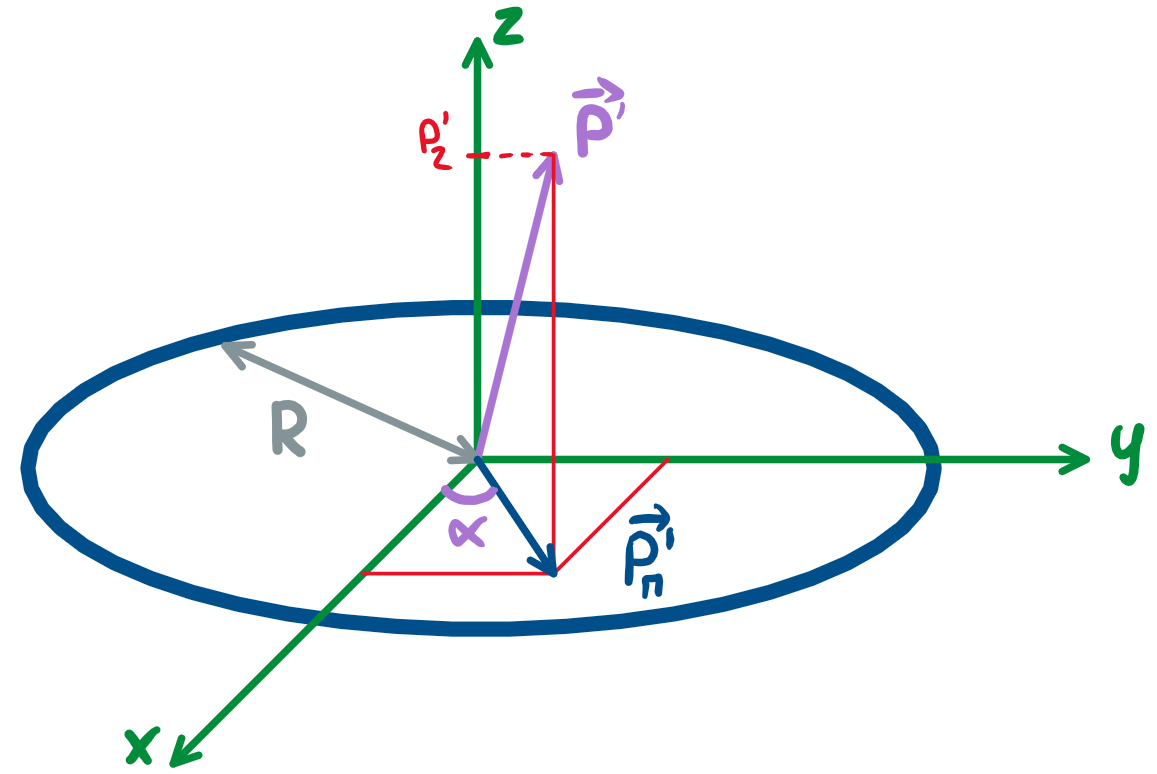
\includegraphics[scale=.4]{Images4/noyau_disque.png}
    \caption{Schéma de la diffusion dans des coordonnées cylindriques}
    \label{fig:Schéma coordonnées sphériques}
\end{figure}
Nous redéfinissons donc le vecteur de la quantité de mouvement de l'électron diffusé :
\[
    \vec{P'} \eq (P'_r \cos(\alpha), P'_r \sin(\alpha), P'_z)
    \qquad \text{avec} \quad P'_r = P \sin(\theta)
\]
On réécrit donc l'expression du facteur de forme définie à la section \ref{sec:noyau_non_ponctuel} comme la transformée de Fourier de la densité de charge $\rho$ :
\[
    F(\vec{q}) \eq \dfrac{1}{\pi R^2}\int_0^{2\pi} \int_0^R \exp[ iP'_r \left(\cos(\alpha)\cos(\phi) + \sin(\alpha)\sin(\phi) \right) ] \; r \dif r \dif\phi
\]
Le résultat de cette intégration est une fonction de Bessel\footnote{En cas de problèmes vis-à-vis de cette notion, contacter le Pr. Grégoire Winckelmans de l'EPL, spécialiste international de la question. Très ouvert et humain, il ne faut pas hésiter à aller directement sonner à son bureau.}, et est simplement l'analogue des sinus cardinaux associés à la diffraction à travers une fente rectangulaire pour une fente circulaire.

Bessel ou pas (même si on préfère pas hn), on peut sortir de ces développements que, selon le modèle d'une densité de charge disque, l'angle auquel apparaît le premier minimum $F(\vec{q})$ est :
\[
    \theta_1 \eq 1.21\dfrac{\lambda}{D}
\]
Nous pouvons comparer ce résultat avec le modèle carré qui, pour rappel, avait une première annulation allant de $1\dfrac{\lambda}{D}$ à $\sqrt{2}\dfrac{\lambda}{D}\approx 1.41\dfrac{\lambda}{D}$. Ainsi, on observe que la moyenne du modèle carré ($1.2\dfrac{\lambda}{D}$) est en fait une bonne approximation du modèle disque.
\begin{figure}[H]
    \centering
    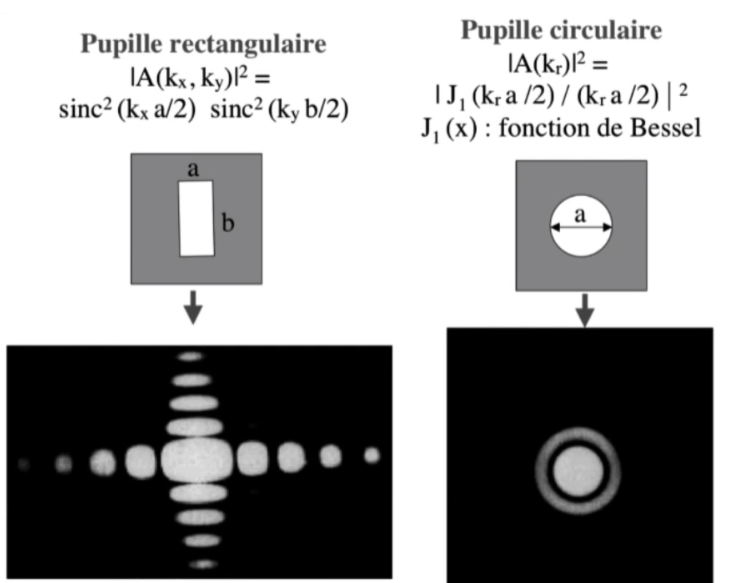
\includegraphics[scale=0.6]{Images4/ComparaisonFente.PNG}
    \caption{Comparaison des figures de diffraction pour des fentes rectangulaire et circulaire. Il est à noter que, pour la diffraction rectangulaire, il manque des interférences : on devrait obtenir une sorte de grille}
    \label{fig:Comparaison fente}
\end{figure}





\subsection{Extraire la distribution de charge depuis la mesure de la section efficace}




On présente donc le graphe de cette transformée. La densité obtenue est quasi une fonction créneau. On comprend maintenant pourquoi il est bien plus simple de définir le rayon du noyau que celui d'un atome. En effet, les charges du noyau sont confinées dans une zone restreinte de l'espace, tandis que les électrons sont distants les uns des autres et suivent des orbites s'étalant radialement parfois sur plusieurs fois le rayon de Bohr.




 \begin{figure}[H]
    \centering
    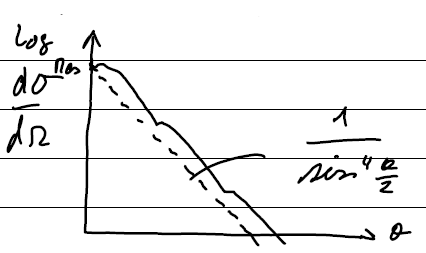
\includegraphics[scale=0.80]{Images4/graphe 1.PNG}
    \caption{Section efficace expérimentale en fonction de l'angle de détection}
    \label{fig:Section efficace expérimentale}
\end{figure}
\begin{figure}[H]
    \centering
    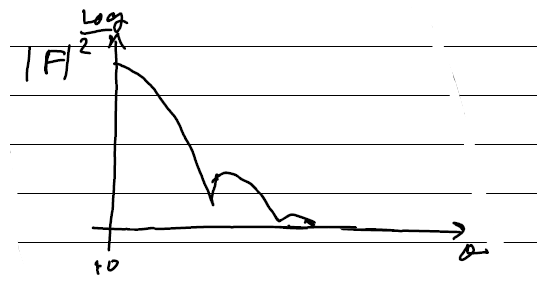
\includegraphics[scale=0.80]{Images4/graphe 2.PNG}
    \caption{Facteur de forme extrait de la section efficace expérimentale en fonction de l'angle de détection}
\end{figure}
 \begin{figure}[H]
    \centering
    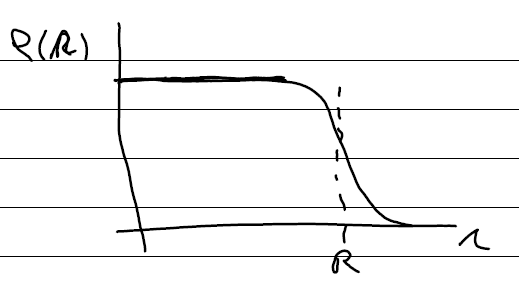
\includegraphics[scale=0.80]{Images4/Fourier.PNG}
    \caption{Transformée de Fourier inverse du facteur de forme}
    \label{fig:Transformée de Fourier}
\end{figure}


    \subsection{Conséquences sur la structure du noyau}


Il est bon à ce stade de rappeler les étapes de notre raisonnement\footnote{On a écrit $\rho(r)$ et non $\rho(\vec{r})$ car la densité de charge est supposée isotrope} : 
\[
\boxed{
    |F(\vec{q})|^2 \; \longrightarrow \; F(\vec{q}) \; \longrightarrow \; \rho(r) \eq \dfrac{1}{2\pi} \int_0^{\infty} \exp(-\vec{q}\cdot \vec{r})
    F(\vec{q}) \dif^3\vec{q}
}
    \qquad r \in [0,R] \quad \text{et R = rayon du noyau}
\]
Nous allons maintenant discuter des résultats obtenus avec nos théories de la densité de charge du noyau. Plus précisément, nous allons les comparer avec les courbes expérimentales obtenues pour $|F(\vec{q})|^2$. Nous allons démarrer nos critiques à l'aide de la figure \eqref{fig : Comparaison entre atomes}, qui représente trois mesures de la diffusion d'un électron sur un noyau de carbone (à 420 {MeV}) et sur un noyau d'oxygène (à \SI{420}{MeV} et \SI{360}{MeV}) :
\begin{figure}[H]
    \centering
    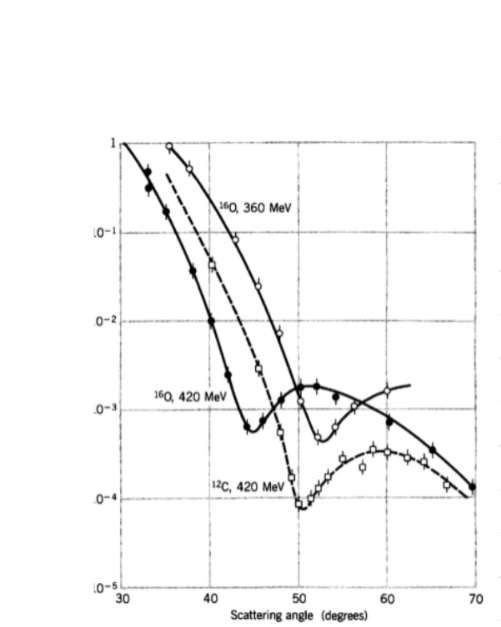
\includegraphics[scale=0.80]{Images4/ComparaisonAtomes.PNG}
    \caption{Comparaison des mesures de section efficace en faisant varier le noyau cible et l'énergie des électrons qui le sondent}
    \label{fig : Comparaison entre atomes}
\end{figure}

Quelques observations sur nos résultats :
\begin{itemize}
    \item On constate sans surprise sur la figure \eqref{fig : Comparaison entre atomes} que l'augmentation de l'angle d'observation (= angle auquel on place le détecteur) provoque une diminution générale (on a parfois des remontées mais légères vu que le graphe est logarithmique) de l'intensité observée (= nombre d'électrons observés à cet angle) et ce peu importe l'énergie de l'électron incident ou l'atome cible. En effet, cette décroissance est attendue de par le terme en  $1/\sin^4(\theta)$ provenant de la section efficace de Rutherford

    \item On observe par contre que la position du premier minimum est fonction de l'énergie des particules incidentes et de l'atome cible. On rappelle que pour des petits angles, en unités naturelles ($\hbar = c = 1$) et pour des particules incidentes ultra-relativistes ($P \approx E$) :
    \[
        \theta \eq \sqrt{2} \dfrac{\lambda}{D} \; \propto \; \dfrac{1}{P D} \; \propto \; \dfrac{1}{E_e D}
    \]
    On constate bien que pour une énergie incidente plus élevée, l'angle du premier minimum est plus faible. On constate également qu'à énergie incidente constante, si on augmente la masse atomique de l'élément cible (en passant du $^{12}C$ au $^{16}O$ ), on a également un minimum pour un angle $\theta$ plus faible : $\theta_m \propto \dfrac{1}{D}$. On voit donc les prémisses d'une relation $D\uparrow \Leftrightarrow M\uparrow$.\\
    \item En étendant le raisonnement à plus d'atomes différents, on s'aperçoit bien de la corrélation entre la taille du noyau\footnote{La taille du noyau n'est pas encore définie univoquement car la densité de charge diminue de façon douce.} et le nombre de nucléons qu'il comporte, donc sa masse. Ici, la figure représente des noyaux pair-pair, c'est à dire comprenant un nombre pair de neutrons et un nombre pair de protons
     \begin{figure}[H]
        \centering
        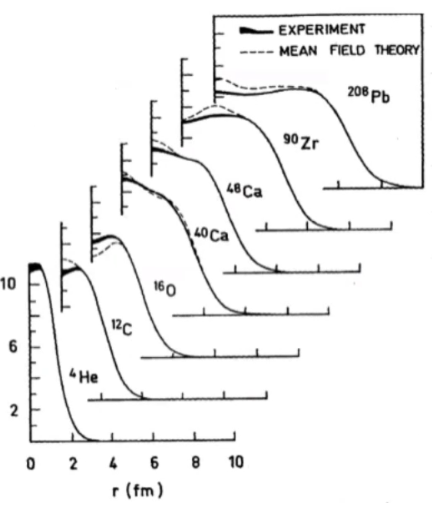
\includegraphics[scale=0.7]{Images4/ComparaisonAtomes2.PNG}
        \caption{Comparaison des densité de charge pour plusieurs atomes pair-pair}
        \label{fig : Comparaison des densités de charge}
    \end{figure}
    \item En regardant maintenant des noyaux de Z très éloignés, on peut conclure que de manière générale :
    \begin{center}
        \boxed{\text{Les noyaux lourds ont une densité de charge plus petite.}}
    \end{center}
    L'origine de ce phénomène sera expliqué plus loin dans le cours même si on sait tous que c'est parce que plus le noyau est lourds, plus il doit comporter de neutrons pour pouvoir être stable (et donc on a moins de protons par unité de volume).
     \begin{figure}[H]
        \centering
        \includegraphics[scale=1.0]{Images4/Noyauxlourds.PNG}
        \caption{Comparaison des densité de charge pour plusieurs atomes de Z fort différents}
        \label{fig : Comparaison des densités de charge noyaux lourds}
    \end{figure}
    \item On peut modéliser la densité de charge par cette expression\footnote{$\rho_0$ variera pour des noyaux autre que pair-pair pour refléter cette diminution de la densité de charge} :
    \[
        \rho(r) \eq \dfrac{\rho_0}{1 + \exp(\dfrac{r - R}{a})}
    \]
    On peut ensuite extraire $R$ comme illustré sur le graphe \ref{fig : Densité de charge} : R est défini comme $\dfrac{\rho(R)}{\rho_0} \equiv \dfrac{1}{2}$. Pour des noyaux pair-pair, on obtient ainsi :
    \[
        \boxed{
            R \eq 1.07\; A^{\dfrac{1}{3}} [\si{fm}] \;\equiv\; r_0A^{\dfrac{1}{3}}
        } \; \text{où A est le nombre de masse atomique}
    \]
    Cette relation nous indique donc que \textbf{le volume du noyau est proportionnel au nombre de nucléons}. Pour le moment, la valeur 1.07 (et donc $r_0$) n'a pas encore de signification physique. Il est à noter qu'en utilisant $r_0=1.2$ à la place de $r_0=1.07$, on obtient une assez bonne correspondance du rayon de tous les noyaux (et plus seulement des noyaux pair-pair).
    \smallskip\\
    Pour mettre des valeurs sur ces notions on obtient une densité de nucléons (proton en neutron confondus) de $\rho_{nucleon} = 2\rho_{proton} = 0.015 \;\text{nucléon}/\si{fm^3}$. On suppose raisonnablement ici que l'interaction entre nucléons est indépendante de la charge des nucléons (voir Isospin plus tard).\\
    Pour conclure, nous pouvons calculer le rayon d'un nucléon
    en reprenant la définition de la densité volumique de nucléons:
    \[
        \rho_{nucleons} \eq \dfrac{A}{4/3 \pi R^3 } \qquad \text{cette valeur est $\pm$ constante pour tous les noyaux}
    \]
    Or, nous avons déduit plus haut que $R \eq r_0A^{\dfrac{1}{3}}$. En injectant ce résultat dans la densité de nucléons:
    \[
        \rho_{nucleons} \eq \dfrac{1}{4/3 \pi r_0^3}
    \]
    En fait, cette expression est exactement l'expression de la densité volumique de de nucléon normalisée à un nucléon. On identifie ainsi le $r_0$ comme le rayon d'un nucléon (avant, cette grandeur n'avait pas de sens physique).\\

    En combinant le fait que le volume du noyau est proportionnel au nombre de nucléon et qu'on peut voir un nucléon comme une boule, on se rend compte que l'image instinctive du noyau comme un ensemble de balles entreposées dans un volume sphérique semble donc fort adaptée !
    \begin{figure}[H]
        \centering
        \includegraphics[scale=1.2]{Images4/DensitéFinale.PNG}
        \caption{Densité de charge finale}
        \label{fig : Densité de charge}
    \end{figure}
\end{itemize}


\subsection{Diffusion à petits angles}


Nous pouvons à partir de la diffusion à petits angles définir le rayon quadratique moyen. En effet, pour de petits angles ($\vec{P}$ est presque parallèle à $\vec{P'} \; \Leftrightarrow \; \vec{q}\;\approx\;\vec{0}$), nous pouvons développer l'exponentielle dans le facteur de forme en une série de Taylor:
\begin{align*}
    F(\vec{q}) &\;\equiv\;
    \int \rho(\vec{R}) \cdot e^{\imag\dfrac{\vec{q} \cdot \vec{R}}{\hbar}} \; \dif^3\vec{R}\\[4pt]
    &\;\approx\;
    \int \rho(\vec{R}) \cdot \bigg( 
    1 + i\dfrac{\vec{q}\cdot\vec{R}}{\hbar} - \dfrac{1}{2!} \left( \dfrac{\vec{q}\cdot\vec{R}}{\hbar}\right)^2
    \bigg) \; \dif^3\vec{R}\\[4pt]
    &\eq
    \int \rho(R) \;\dif^3\vec{R}
    \;+\;
    \int \rho(R)  i\dfrac{\vec{q}\cdot\vec{R}}{\hbar} \; \dif^3\vec{R}
    \;-\;
    \int \rho(R)  \dfrac{1}{2!} \left( \dfrac{\vec{q}\cdot\vec{R}}{\hbar}\right)^2  \; \dif^3\vec{R}
    \qquad \text{avec} \quad \rho(\vec{R}) \eq \rho(R)\\[4pt]
    &\eq
    1
    \;+\;
    \underbrace{\int \rho(R)  i\dfrac{\vec{q}\cdot\vec{R}}{\hbar} \; \dif^3\vec{R}}_{\equiv \; \alpha} 
    \;-\;
    \underbrace{ \int \rho(R)  \dfrac{1}{2!} \left( \dfrac{\vec{q}\cdot\vec{R}}{\hbar}\right)^2  \; \dif^3\vec{R}}_{\equiv \; \beta}
\end{align*}
Nous pouvons développer les deux intégrales $\alpha$ et $\beta$ en prenant $\vec{q}\; \slash{}\slash{}\; \hat{z} \;\Leftrightarrow\; \vec{q}\cdot\vec{R} \eq qR\cos(\theta)$. On peut en effet choisir nos axes car nous intégrons sur tout l'espace :
\begin{align*}
    \alpha &\;\equiv\;
    \int \rho(R)  i\dfrac{\vec{q}\cdot\vec{R}}{\hbar} \; \dif^3\vec{R}\\[4pt]
    &\eq
    \int \rho(R)  i\dfrac{qR\cos(\theta)}{\hbar} \; R^2dR \;\sin(\theta)d\theta \; \dif\phi\\[4pt]
    &\eq
    \dfrac{iq}{\hbar} \int_0^{2\pi} \dif\phi \; \int_0^{\pi} \cos(\theta) \sin(\theta) d\theta \;\int_0^{+\infty}\rho(R) R^3 dR \\[4pt]
    &\eq 0 \qquad \text{car on intègre $\sin(2\theta)=2\sin(\theta)\cos(\theta)$ sur une période}
    \\[7pt]
    \beta &\;\equiv\;
    \int \rho(R)  \dfrac{1}{2!} \left( \dfrac{\vec{q}\cdot\vec{R}}{\hbar}\right)^2  \; \dif^3\vec{R}\\[4pt]
    &\eq
    \int \rho(R)  \dfrac{1}{2!} \left( \dfrac{qR\cos(\theta)}{\hbar}\right)^2  \; R^2dR \;\sin(\theta)d\theta \; \dif\phi\\[4pt]
    &\eq
    \dfrac{q^2}{2\hbar^2}
    \int_0^{2\pi} \dif\phi \; \int_0^{\pi} cos^2(\theta) \sin(\theta) d\theta \;\int_0^{+\infty}\rho(R) R^4 dR \\[4pt]
    &\eq ... \eq \dfrac{2\pi}{3}\dfrac{q^2}{\hbar^2} \;\int_0^{+\infty}\rho(R) R^4 dR
\end{align*}
Ainsi, pour des diffusions à petits angles:
\[
    F(\vec{q}) \;\approx\; 1 - \dfrac{2\pi}{3}\dfrac{q^2}{\hbar^2(=1)} \;\int_0^{+\infty}\rho(R) R^4 dR
\]
On peut encore simplifier cette expression en introduisant la valeur moyenne du carré du rayon:
\begin{align*}
    <R^2> &\;\equiv\;
    \dfrac{ \int R^2 \rho(R) \; \dif^3\vec{R} }{ \int \rho(R) \; \dif^3\vec{R} }\\[4pt]
    &\eq
    \int R^2 \rho(R) \; \dif^3\vec{R}
    \qquad \text{par définition de la densité de charge}\\[4pt]
    &\eq
    \int_0^{2\pi}\dif\phi \int_0^{\pi} \sin(\theta) d\theta \int_0^{+\infty}\rho(R) R^4dR\\[4pt]
    &\eq 
    4\pi \int_0^{+\infty}\rho(R) R^4dR\\[4pt]
    &\approx \dfrac{4\pi\int_0^R R^4dR}{4\pi\int_0^R R^2dR} \qquad \text{Pour une densité de la forme d'une marche de 0 à R}\\[4pt]
    &\approx \dfrac{3}{5}R^2
\end{align*}
En injectant le résultat dans l'expression du facteur de forme pour de faibles $\vec{q}$:
\begin{equation}
    \boxed{
    F(\vec{q}) \;\approx\; 1 + \dfrac{q^2}{6\hbar^2} <R^2>
    \quad \Leftrightarrow \quad
    <R^2> \eq -6\hbar^2 \left. \fdif{F(q)}{(q^2)}\right|_{q^2=0}
    }
    \label{deriv_fact_forme}
\end{equation}
Tout cela semble assez naturel :  en effet, les électrons sonde que nous employons ne <<voient>> que la surface effective des atomes qu'ils rencontrent. Ce la se traduit par l'apparition du rayon carré moyen, il correspond au rayon de la moyenne de la surface observée, on mesure en réalité $\expval{R^2}$.\\
Alors, en quoi le rayon quadratique moyen diffère-t'il du rayon classique? Prenons un exemple : le noyau de deuton (1 proton et un neutron) a une forme de cigare, lors d'une collision entre un électron sonde et cette distribution de charge, l'électron percevra en moyenne une sphère de rayon R, où R représente donc le <<diamètre>> du cigare, sa plus grand longueur. La mesure du rayon quadratique moyen a donc bien plus de sens.\\
\begin{figure}[H]
    \centering
    \includegraphics[scale=0.8]{Images4/deutérium.png}
    \caption{Noyau du deutérium}
\end{figure}
Ainsi, la pente du facteur de forme (sa dérivée donc) pour de petits angles de diffusion (ou de façon équivalente pour de petites valeurs de $q$), fournit une information sur le \textbf{rayon quadratique moyen} $\sqrt{<R^2>}$ par la relation \ref{deriv_fact_forme}. Cette information sur le rayon de la densité de charge $\rho(R)$ est accessible sans faire de transformée inverse de Fourier des données.\\
En repartant des relations établies précédemment, on peut établir une relation entre $R$ et $A^{1/3}$. On observe cette droite\footnote{La droite n'est pas exactement celle qui approxime au mieux les données car on la force à passer par l'origine} expérimentalement :
\begin{figure}[H]
    \centering
    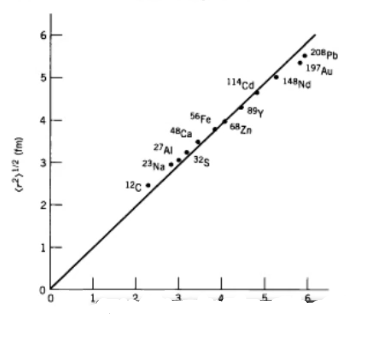
\includegraphics[scale=1.2]{Images4/DroiteAR.PNG}
    \caption{Graphe du rayon quadratique moyen observé en fonction de $A^{1/3}$ tel que A est le nombre de masse}
\end{figure}
\begin{align*}
    R &\eq \sqrt{\dfrac{5}{3}} \sqrt{\expval{R^2}}\\
    &\eq \sqrt{\dfrac{5}{3}} aA^{1/3} \quad \text{où $a$ est la pente de la droite mesurée expérimentalement}
\end{align*}
En général :
\[
    \boxed{
        R \eq 1.2 A^{1/3}
    }
\]
Pour des noyaux pair-pair :
\[
    \boxed{
        R \eq 1.07 A^{1/3}
    }
\]



\section{La stabilité nucléaire}

\subsection{Mesure de la masse des noyaux}

A quoi peut nous servir la masse expérimentale des noyaux? Connaissant la masse des noyaux et les masses individuelles de ses constituants, nous pouvons aisément déduire l'énergie de liaison des nucléons dans le noyau!

\subsubsection{Le spectromètre de masse}


La mesure de la masse d'un ion se fait à l'aide du spectromètre de masse. Nous allons un peu nous attarder sur cet appareil et rappeler son principe de fonctionnement.
 \begin{figure}[H]
    \centering
    \includegraphics[scale=0.5]{Images4/Spectromètre_masse.png}
    \caption{Schéma d'un spectromètre de masse}
    \label{fig:Schéma_spectrometre_masse}
\end{figure}
L'utilisation d'un spectromètre de masse permet de déterminer le rapport entre la masse d'un ion et sa charge (donc, si nous connaissons sa charge nous connaîtrons sa masse).\\
Une source produit donc un faisceau d'ions qui rentre dans un espace dans lequel règnent un champ magnétique et un champ électrique. Les ions qui nous intéressent sont ceux qui iront tout droit (dans un trou percé dans une paroi), c'est-à-dire sur lesquels aucune force ne s'applique. En vertu de la force de Lorentz:
\[
    \vec{F}_{EM} \;\equiv\;
    q\vec{E} + q\vec{v}\cross\vec{B_1}
    \quad \Leftrightarrow \quad
    E\eq vB_1
    \quad \Leftrightarrow \quad
    v \eq \dfrac{E}{B_1}
\]
Nous connaissons donc la vitesse des ions qui arrivent dans un deuxième espace ou règne un champ magnétique perpendiculaire à la vitesse de ces ions. Par conséquent, dans cet espace, l'ion décrit un cercle de rayon $\rho$. En égalisant la force centrifuge et la force de Lorentz dans cet espace:
\[
    \dfrac{Mv^2}{\rho} \eq q |\vec{v}\cross\vec{B_2}|
    \quad \Leftrightarrow \quad
    \dfrac{M}{q} \eq \rho v B_2 \eq \rho \dfrac{B_1}{E} B_2 
\]
La mesure du rayon se fait à l'aide d'une plaque photographique placée sur la trajectoire de l'ion. Connaissant la charge des ions, nous connaissons leur masse et, a fortiori, nous connaissons la masse des noyaux des atomes en négligeant la masse des électrons.


\subsubsection{Masse des noyaux et énergie de liaison}


Nous rappellerons ici ce que nous avions vu dans l'introduction sur la masse des noyaux. Soit un atome avec A nucléons, Z protons et Z électrons. En unités naturelles, sa masse M(A,Z) s'écrit:
\begin{align*}
    M(A,Z) 
    &\eq
    m(A,Z) + Z.m_e - E^{\text{atome}}_{\text{liaison}} \qquad \text{tel que} \; m(A,Z) \eq m_{\text{noyau}}\\
    &\eq
    Z.m_p + (A-Z)m_n - E^{\text{nucléaire}}_{\text{liaison}} + Z.m_e - E^{\text{atome}}_{\text{liaison}}
\end{align*}
Définissons l'énergie de liaison de l'atome par $B$. Cette énergie de liaison totale est largement dominée par l'énergie de liaison nucléaire de sorte que dans la suite, on approximera B comme l'énergie de liaison du noyau. Cette énergie de liaison est généralement négligeable devant l'énergie de masse.
\[
    B \eq
    E^{\text{atome}}_{\text{liaison}}+E^{\text{noyau}}_{\text{liaison}}
    \;\approx\; E^{\text{noyau}}_{\text{liaison}}
\]

En guise d'exemple, considérons le deutérium, atome formé d'un proton,d'un neutron et d'un électron. Évaluons l'énergie de liaison de son noyau, le deuton. On a 
    \[
        M(^{2}D)=2,014~u
    \] 
où $u=\dfrac{1}{12}M(^{12}_{}C)=931,495\dfrac{\si{MeV}}{c^2}=1,66054.10^{-27}kg$\\[0,2cm]
Nous connaissons donc la masse du proton (via la masse de l'atome d'hydrogène), la masse du deuton (via spectromètre de masse). Pour déterminer la masse du neutron, nous avons besoin de l'énergie de liaison du deuton. Pour mesurer cette énergie, nous avons deux options:
\begin{itemize}
    \item En bombardant des neutrons sur des protons, nous aurons éventuellement une fusion dont il résultera un deuton et un photon : $n+p \rightarrow ^2D+\gamma$. L'énergie de liaison sera donc l'énergie du photon émis par la réaction.
    
    \item On peut également envoyer des photons sur des noyaux de deutérium. Éventuellement, si ces photons on une énergie suffisante, il se produira la fission du deuton (nous regarderons l'apparition de protons) : $^2D+\gamma \rightarrow n+p$. L'énergie seuil du photon qui permet d'induire la réaction sera l'énergie de liaison du deuton.
\end{itemize}
Nous obtenons ainsi comme énergie de liaison du deuton : $E^{\text{deuton}}_{\text{liaison}} \eq \SI{2.227}{MeV}/c^2$


\subsection{La radioactivité}


Nous allons ici rappeler les procédés radioactifs qui nous seront utiles pour la suite de la section.

\subsubsection{Rayonnement $\alpha$}

Le rayonnement alpha, qui consiste en l'émission de noyaux d'Hélium par des noyaux d'atomes, est très vite arrêté par la matière (après une feuille de papier). L'énergie des particules $\alpha$ est discrète : on observe ainsi des raies d'émission caractéristiques d'un élément. La réaction s'écrit comme suivant, avec $Q$, l'énergie de la réaction :
\[
    ^{A}_{Z}X \;\rightarrow\; ^{A-4}_{Z-2}Y \;+\; ^{4}_{2}He \quad(+Q)
\]
Bilan énergétique d'une désintégration $\alpha$:
\begin{align*}
    Q &\eq
    T_Y + T_\alpha \eq [M_{at}(X)-M_{at}(Y)-M_{at}(He)]c^2 \;>\;0\\
    Q &\eq B(A-4,Z-2)+B(^{4}_{2}He)-B(A,Z) \;>\;0
\end{align*}
On voit ainsi que la réaction est exothermique : elle est donc possible sans apport externe d'énergie, ce qui veut dire qu'elle est \textbf{spontanée}. En fait, le processus spontané de fission par émission de particules $\alpha$ correspond à un effet tunnel (on verra peut-être ça plus en détail) et le temps de vie d'un atome est fonction de la hauteur et de l'épaisseur de la barrière de potentiel.

\subsubsection{Rayonnement $\beta$}


Le rayonnement $\beta$ est caractérisé par l'émission d'un électron et d'un antineutrino (rayonnement $\beta^-$) ou d'un positron et d'un neutrino (rayonnement $\beta^+$) par le noyau. Contrairement au rayonnement $\alpha$, le spectre d'énergie du rayonnement $\beta$ est continu : l'électron émis peut prendre n'importe quelle énergie.\\
Dans le cas du rayonnement $\beta^-$, la réaction s'écrit:
\[
    ^{A}_{Z}X \rightarrow ^{A}_{Z+1}Y + e^- + \bar{\nu}_e
\]

\subsubsection{Rayonnement $\gamma$}


Possède un pouvoir de pénétration supérieur aux rayonnements $\alpha$ et $\beta$ (quelques centimètres de plomb). A l'instar du rayonnement $\alpha$, le spectre du rayonnement $\gamma$ est caractérisé par des raies : l'énergie est discrète.\\
Le rayonnement $\gamma$ peut s'obtenir par stabilisation du noyau nouvellement formé à la suite d'un autre rayonnement, comme sur la figure \eqref{fig:Rayonnement gamma}.
\begin{figure}[H]
    \centering
    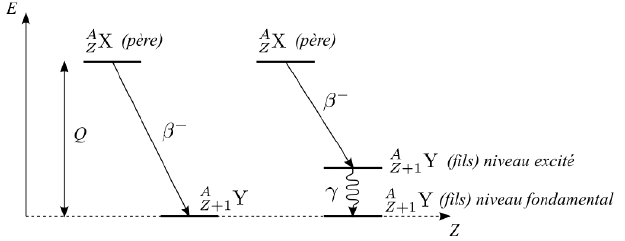
\includegraphics[scale=0.7]{Images1/gamma.PNG}
    \caption{Rayonnement $\gamma$}
    \label{fig:Rayonnement gamma}
\end{figure}


\subsection{La stabilité des noyaux : vallée de stabilité}

Nous allons dans cette section utiliser des graphes $(p,n)$ où sont répertoriés l'ensemble des noyaux stables ($\equiv$ les noyaux qui \textbf{ne se désintègrent pas spontanément}) et les noyaux instables ($\equiv$ les noyaux ayant des temps de vie non-négligeables : $\tau \in [ps,\text{âge de l'univers}]$). Bien qu'un noyau devrait à priori pouvoir occuper n'importe quel point de l'espace $(p,n)$, on observe en pratique une zone, appelée \textbf{vallée de stabilité} où sont tous les noyaux stables qui est entourée d'une zone où se trouvent les noyaux instables (figure \ref{fig:Stabilité noyaux 1}). Il est à noter que, parfois, le nombre de neutrons $N$ est remplacé par le nombre atomique de masse $A$ dans le diagramme.
\begin{figure}[H]
    \centering
    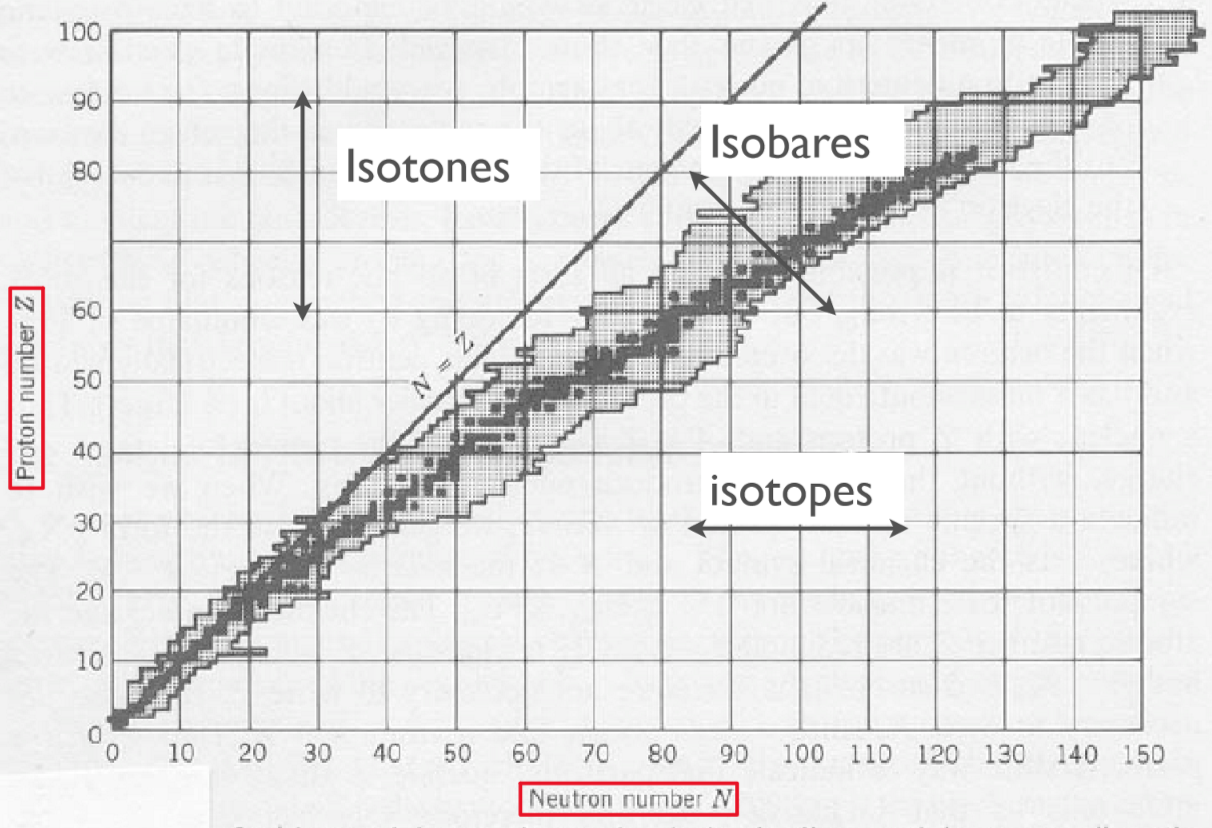
\includegraphics[scale=0.3]{Images4/Stabilite_noyaux_1.png}
    \caption{Graphe $(p,n)$ - les noyaux stables sont montrés en noir et les radionucléides connus en gris}
    \label{fig:Stabilité noyaux 2}
\end{figure}
On peut être surpris que la vallée de stabilité ne suive pas la droite $Z=n$ (tracée en traits continus) et qu'à partir d'une certaine valeur de $Z$, il n'existe plus de noyaux stables. Ces deux phénomènes devront être expliqués par notre modèle du noyau.\\

On peut également établir des relations entre les noyaux qui nous seront utiles pour caractériser les transitions :
\begin{itemize}
    \item isobares : ensemble de noyaux avec le même nombre de nucléons $A$
    \item isotones : ensemble de noyaux avec le même nombre de neutrons $A-Z$
    \item isotopes : ensemble de noyaux avec le même nombre de protons $Z$ 
\end{itemize}
On observe 3 types de fissions spontanées (créations de 2 noyaux fils) :
\begin{itemize}
    \item Émission d'un neutron (apparaît quand le noyau père a un faible temps de vie)
    \item Émission d'un proton (phénomène plus rare que l'émission d'un neutron)
    \item Émission d'une particule $\alpha$
\end{itemize}
Un autre type de transmutation est réalisé à l'aide des rayonnements $\beta^+$ et $\beta^-$:
\begin{figure}[H]
    \centering
    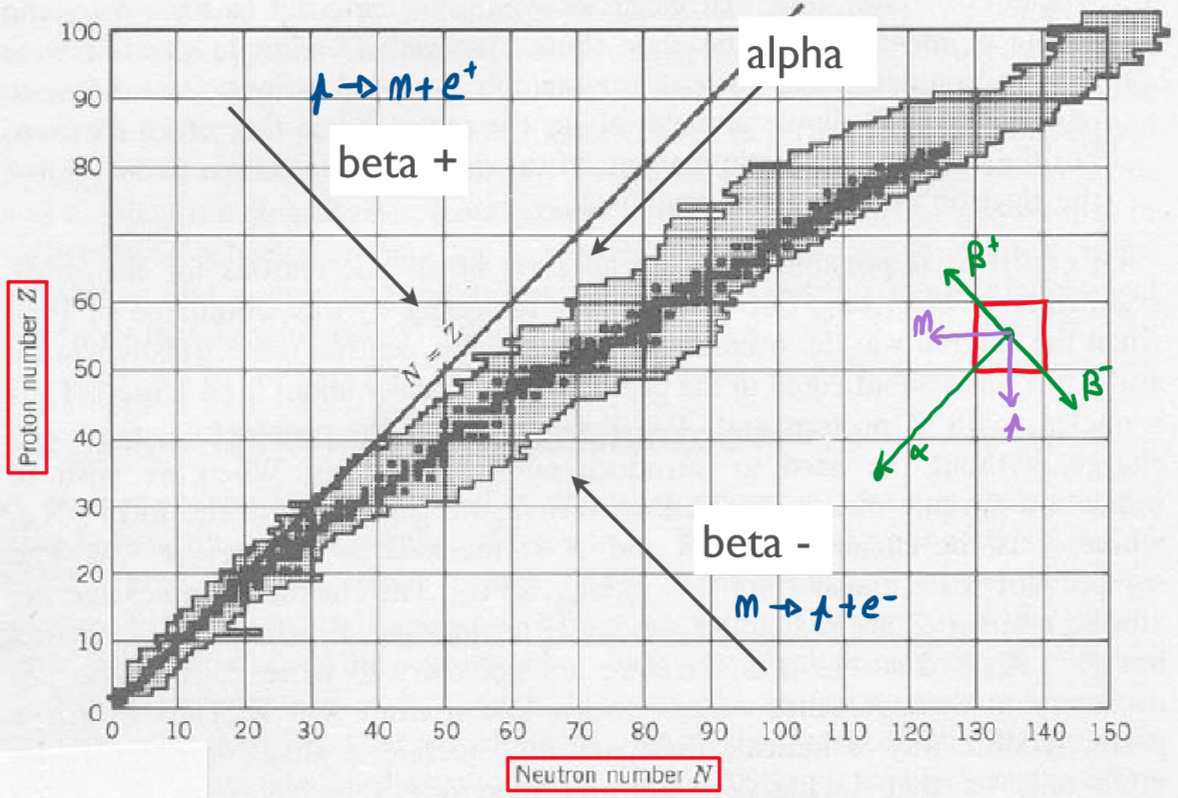
\includegraphics[scale=0.3]{Images4/Stabilite_noyaux_2.png}
    \caption{Graphe $(p,n)$ - les noyaux stables sont montrés en noir et les radionucléides connus en gris. On a également illustré le résultat des transitions}
    \label{fig:Stabilité noyaux 1}
\end{figure}
En outre, il existe des noyaux pseudo-stables : c'est-à-dire que, pour un même nombre de protons et neutrons (=même noyau), il existe deux agencements possibles des nucléons dont l'un est stable et l'autre instable. Ce type de noyau est de plus en plus présent lorsque $A$ augmente.

\subsection{Les niveaux d'énergie des noyaux}
Le parallèle avec la physique atomique est direct : les noyaux ont également des niveaux d'énergie avec un état fondamental et des états excités\textcolor{red}{Demander au prof à quoi correspond un état excité : un arrangement différent? Des vibrations entre les nucléons? Vibrations comme dans un cristal? Cette question a aussi un impact sur le paragraphe juste au-dessus}, les transitions entre ces niveaux se font via l'émission ou l'absorption d'un photon. Il y a tout de même des différences car on peut également observer des <<transitions entre atomes>>, via les phénomènes de désintégration $\alpha$ et $\beta$ mentionnés précédemment.

\begin{figure}[H]
    \centering
    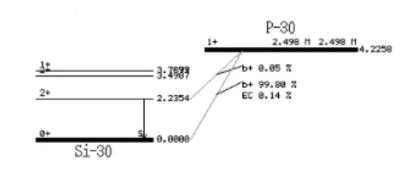
\includegraphics[scale=1.3]{Images4/NiveauxAtomes.PNG}
\end{figure}

On discute ici le cas assez général de la transition entre le $^{30}P$ et le $^{30}Si$. On a donc une désintégration $\beta^+$ avec émission d'un positron et d'un neutrino.
\[
    ^{30}P \; \longrightarrow \; ^{30}Si \; + \; e^+ \; + \; \nu_e
\]
Comme on peut le lire sur le diagramme, la transition vers le fondamental domine largement avec $99\%$ de probabilité.\\
On peut également lire $EC = 0.14\%$ ; EC signfie \emph{electron conversion} et renvoie à un phénomène relativement analogue de désintégration. On sait que les électrons des couches s ont une probabilité non-nulle de se trouver au centre du noyau, lorsque cela se produit il peut se produire cette réaction :
\[
    e^- \; + \; ^{30}P \; \longrightarrow \; ^{30}Si \; + \; \nu_e
\]
On a donc réaction entre l'électron et un proton du noyau via le recouvrement de leurs fonctions d'onde. La réaction donne un neutron et un neutrino électronique. Le bilan d'énergie est donc différent car l'énergie "gagnée", la différence d'énergie entre les deux niveaux $\Delta E$, doit être répartie entre seulement 2 acteurs,le silicium et le neutrino, et non 3.\\
Pour information, les transitions possibles sont déterminées par des règles de sélection de façon tout à fait analogue à la physique atomique. En effet, pour la désintégration du $^{30}P$ en $^{30}Si$, on a des transitions de spin possibles (on a l'équivalent de termes, je crois, sur la gauche de l'état : $1+$ par exemple) et la transition $1+ \rightarrow 0+$ est plus probable devant la transition $1+ \rightarrow 2+$







\section{Étude du deuton ($\equiv$ noyau du deutérium)}

Maintenant que nous en savons plus sur les résultats des expériences visant à mesurer la structure interne du noyau, nous devons nous attarder à établir un modèle mathématique du noyau. Notre modèle débute comme toujours par le cas le plus simple, c'est-à-dire dans notre cas le premier état lié entre des nucléons. Nous allons donc étudier le noyau du deutérium\footnote{This sounds like hydrogen with extra steps}, qui est composé d'un proton et d'un neutron.\\
Il est à noter que nous considérons dans ce modèle le proton et le neutron comme deux particuler élémentaires : les quarks n'entrent pas encore en jeu. Et, pour encore plus de simplicité, on suppose que le proton et le neutron sont deux particules ponctuelles.\\


\subsection{Fonction d'onde associée à deux particules}


Pour débuter dans notre modèle quantique du noyau, nous devons connaître la fonction d'onde associée à deux particules. Il est à noter que cette fonction peut s'écrire de différentes façons en fonction du spin des constituants. Mais, dans notre cas, le proton et le neutron sont deux fermions de spin $1/2$ (on considère ces résultats pour acquis).\\

Un noyau n'est pas ponctuel ; nous l'avons démontré. Par conséquent, un état lié proton-neutron aura un certain rayon. Mais, par la diffusion d'électrons, tout ce que nous mesurons et le rayon quadratique moyen $R = \sqrt{<r^2>}$. Nous prenons également pour acquis que, dans le cas du deuton, $R= \SI{2.1}{fm}$.

Remarquons que, bien que nous notons $R$, la quantité mesurée correspond plus à la distance entre le proton et le neutron qu'au rayon (le deuton est fortement oblong, et donc pas du tout sphérique... pour des atomes plus lourds, l'approximation par une sphère est bien plus valable). En effet, lorsque nous procédons à la diffusion d'électrons par le noyau, ce que nous mesurons dépend de l'orientation relative du noyau et du faisceau, nous mesurons une surface effective!

En fait, nous avons un problème à 2 corps ayant une même masse (à peu de choses près):
\begin{figure}[H]
    \centering
    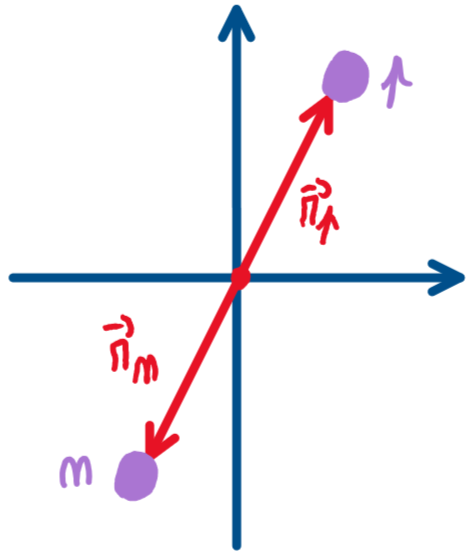
\includegraphics[scale=0.3]{Images4/noyau_deuton.png}
    \caption{Représentation schématique d'un noyau de deuton}
\end{figure}
Les paramètres importants dans le problème à deux corps sont $r=R$, le rayon effectif du système à deux corps et la masse réduite $\mu \;\equiv\; \dfrac{m_pm_n}{m_p+m_n} \;\approx\; \dfrac{m_n}{2} \eq \dfrac{m_p}{2}$. Nous supposons aussi que le potentiel d'interaction nucléon/nucléon est central : $V(\vec{r})\equiv V(r)$. Dans un tel contexte, la fonction d'onde du système $\Psi_{12}$, avec $1$ décrivant le proton et $2$ décrivant le neutron est:
\begin{align*}
    \Psi_{12} &\eq
    \Psi(\vec{r}_1,\vec{r}_2,\vec{s}_1,\vec{s}_2) \qquad \text{avec $\vec{s}_i$ le spin de la particule $i$}\\
    &\eq
    \Psi(r,\theta,\phi,\vec{s}_1,\vec{s}_2)   \qquad \text{en passant en coord. sphériques (potentiel central) , } \quad r \;\equiv\; |\vec{r}_1-\vec{r}_2|\\
    &\eq
    \chi(r) \cdot Y^m_l(\theta,\phi) \cdot \alpha(\text{spin}) \qquad \text{le potentiel est central et ne dépend donc que de $r$\footnotemark}
\end{align*}
\footnotetext{Comme vu dans la partie atomique, si un potentiel est central, alors la partie angulaire des fonctions d'onde est décrite par des harmoniques sphériques.}
Il est à noter que la fonction $\alpha(\text{spin})$ devra respecter la loi de conservation du moment cinétique total et que par `spin', nous désignons le spin total du système.\\


\subsection{Effet de la permutation de deux particules et fonction de spin pour le deuton}\label{Permut_deuton}


Que se passe-t-il lors de l'échange du proton avec le neutron? Manifestement, cela revient à changer les vecteurs de base : $\vec{r} \rightarrow -\vec{r}$, ce qui est également le résultat de l'opération de parité $P$. Pourquoi introduire $P$? Car nous connaissons son action sur les harmoniques sphériques (si on admet, et ce n'est pas une hypothèse anodine, que les harmoniques sphériques décrivent bien les coordonnées angulaires de notre système car pour cela on admet un potentiel central):
\[
    (n,p)\rightarrow (p,n) \quad \Rightarrow \quad
    Y^m_l(\theta,\phi) \rightarrow P\left[ Y^m_l(\theta,\phi) \right] 
    \eq Y^m_l(\pi-\theta,\pi+\phi) \eq (-1)^l Y^m_l(\theta,\phi)
\]
On voit donc que la partie angulaire de la fonction d'onde $\Psi_{12}$ est influencée par l'inversion de deux particules, ce qui n'est pas le cas de la partie radiale $\chi(r)$ car $r$ est défini comme la distance entre le proton et le neutron et ne varie donc pas lorsqu'on échange ces deux particules.\\
Qu'en est-il de la fonction de spin $\alpha$(spin)? Pour étudier l'effet de l'échange des deux particules sur le spin, nous devons connaître le spin total du système:\footnote{Nous pouvons faire un lien brillant avec le cours de théorie des goupes! En fait, ce que nous faisons est la décomposition du moment cinétique dans sa base `naturelle' vers la base couplée: $\ket{j_1,m_1} \otimes \ket{j_1,m_1} \eq \oplus_i c_j \ket{J_j,M}$ où les $c_j$ sont les coefficients de Clebsch-Gordan. Mais cette décomposition est en fait la réduction d'un produit tensoriel en une somme directe (symbolisée par $\oplus)$ de représentations irréductibles.}
\[
    \vec{\dfrac{1}{2}} + \vec{\dfrac{1}{2}} \eq \vec{0}, \: \vec{1}
\]
On peut remarquer que le nombre de `projections' est préservé par cette décomposition : à gauche de l'égalité, nous avons $2\cdot 2$ projections tandis qu'à droite, nous avons $3+1$ projections ($\vec{1}$ est un état triplet tandis que $\vec{0}$ est un état singlet).\\

Nous nous intéressons, nous, à la valeur du spin du système couplé et à la symétrie/l'antisymétrie de sa fonction d'onde. Ainsi, nous pouvons représenter les fonctions d'onde de spin des états singlet et triplet, avec $\alpha(J,M_J=m_1+m_2)$ la fonction de spin et $\Psi_1\uparrow$ signifiant que la particule 1 est de spin up\footnote{Il est à noter que les coefficients devant les fonctions d'onde sont les coefficients de Clebsch-Gordan} :
\begin{itemize}
    \item s=1 : état triplet
    \begin{align*}
        \alpha (1,1)  &\eq \Psi_1\uparrow \Psi_2\uparrow \\
        \alpha (1,0)  &\eq  \dfrac{1}{\sqrt{2}} \left[ \Psi_1\uparrow\Psi_2\downarrow +  \Psi_1\downarrow\Psi_2\uparrow\right]\\
        \alpha (1,-1) &\eq \Psi_1\downarrow\Psi_2\downarrow
    \end{align*}
    \item s=0 : état singlet
    \begin{equation}
        \alpha (0,0)  \eq  \dfrac{1}{\sqrt{2}} \left[ \Psi_1\uparrow\Psi_2\downarrow -  \Psi_1\downarrow\Psi_2\uparrow\right]
    \end{equation}
\end{itemize}
Ainsi, sous l'échange du neutron avec le proton, la fonction d'onde de l'état triplet (resp. singlet) est symétrique (resp. antisymétrique):
\begin{align*}
    P_{12} \left[ \alpha(1) \right] &\eq +\alpha(1) \qquad \text{L'état de spin 1 est symétrique}\\
    P_{12} \left[ \alpha(0) \right] &\eq -\alpha(0) \qquad \text{L'état de spin 0 est antisymétrique}
\end{align*}
Cette symétrie de la fonction de spin est importante car, expérimentalement, le spin du deuton\footnote{Le spin (à l'état fondamental) des particules composées de plusieurs particules élémentaires, comme le proton, le neutron, tout noyau atomique ou encore tout atome, est constitué des spins des particules élémentaires qui les composent, auquel s'ajoute le moment cinétique orbital de ces différentes particules élémentaires [Wikipédia - spin]} est 1 : $\vec{J}_{\text{deuton}} \eq 1$. Le spin du deuton provient donc de deux origines : le spin $\vec{s}$ des particules individuelles et le moment angulaire $\vec{l}$ : $\vec{J}_{\text{deuton}} \eq \vec{s}+\vec{l}$. Nous devons donc étudier les différentes combinaisons possibles de $\vec{s}$ et $\vec{l}$ pour que le spin du deuton soit $\vec{1}$, comme l'impose l'expérience:
\begin{itemize}

    \item Si $s=0$ et $l=0$. Cet état n'existe pas car, et on le sait expérimentalement, son potentiel ne permet pas d'héberger un état lié. Le potentiel total qui agit sur les nucléons est $V_{np} \eq V(r)<0$, bien qu'attractif, n'est pas assez profond pour qu'il y ait un état lié\\[4pt]
    
    \item Si $s=1$ et $l=0$, alors le potentiel total qui agit sur les nucléons est $V_{np} \eq V(r) + f(r) \cdot (\vec{\sigma}_1 \cdot \vec{\sigma}_2)$ avec $V(r)$ le potentiel lié à la force forte et $f(r)$ un terme de couplage de spin. $\vec{\sigma}_i$ désigne la matrice de Pauli associée au vecteur de spin, on a donc : $\vec{S_i} = \dfrac{\hbar}{2}\vec{\sigma}_i$ (le facteur 1/2 est simplement absorbé dans $f(r)$). Ici le produit des matrices de Pauli vaut 1.  En fait, $f$ doit être suffisamment négatif (il doit suffisamment abaisser le potentiel total) pour qu'un état lié soit possible. Il est à noter qu'une telle forme de potentiel est compatible avec le cas $(s=0,l=0)$ où le produit des matrices de Pauli est nul.\\[4pt]
    
    \item  Si $s=0$ et $l=1$, alors le potentiel total qui agit sur les nucléons est toujours $V_{np} \eq V(r) + f(r) \cdot (\vec{\sigma}_1 \cdot \vec{\sigma}_2)$. Cependant, contrairement au cas $(s=1,l=0)$, le produit des matrices de Pauli $\vec{\sigma}_1 \cdot \vec{\sigma}_2$ vaut $-1$ (les spins sont opposés) et, par conséquent, le terme de couplage de spin est positif : il rehausse la valeur du potentiel $V_{np}$, ce qui ne permet donc pas de créer un état lié (le puits d'énergie est encore moins profond que le cas $(s=0,l=0)$ qui n'était déjà pas lié)\\[4pt] 
    %La grande question qui demeure c'est pourquoi on a pas considéré cette correction de spin dans le cas l = 0 s = 0?
    
\end{itemize}

Nous avons donc un premier modèle du potentiel entre deux nucléons qui prend en compte l'interaction de spin. Discutons maintenant de la validité de ce modèle, de ce qu'il permet de prédire.\\

Dans le potentiel $V_{np} \eq V(r) + f(r) \cdot (\vec{\sigma}_1 \cdot \vec{\sigma}_2)$, le terme $f$ est donc le couplage de spin. En fait, il s'agit du même terme que celui de la correction hyperfine de l'atome d'hydrogène, à ceci près que, ici, ce terme n'est pas correctif mais déterminant : $\mathcal{O}(V(r)) \;\approx\; \mathcal{O}(f(r))$.

Puisqu'il existe un état lié $n/p$, il est légitime de se demander s'il existe des états liés $n/n$ ou $p/p$ (uniquement deux particules!). D'un point de vue observationnel, aucun de ces deux cas n'existe. Pour l'état lié $p/p$, on pourrait argumenter que c'est l'interaction coulombienne qui empêche cet état (bien qu'en pratique, ce n'est pas ça qui détermine l'abscence de cet état lié). Cependant, il n'y a, a priori, aucune raison pour que l'état $n/n$ n'existe pas.\\
En fait, ces états liés $n/n$ ou $p/p$ n'existent pas à cause du principe d'incertitude de Pauli qui peut se formuler comme <<\textit{2 fermions identiques ne peuvent pas avoir les même nombres quantiques}>>. Une façon d'assurer cela est d'imposer que la fonction d'onde soit antisymétrique sous l'échange de deux particules (sinon on ne pourrait pas distinguer les deux fermions) : $\Psi_{12} \eq -\Psi_{21}$\\

Qu'en est-il de la fonction d'onde des état $n/n$ et $p/p$?
\begin{itemize}
    \item pour $s=1$ et $l=0$, la partie de la fonction d'onde qui nous intéresse est :
    \begin{align*}
        P_{12} \left[ \Psi_{N_1N_2} \right] &\eq
        P_{12} \left[ R_{N_1N_2} \cdot Y_0^m \cdot \alpha_{N_1N_2}(1)  \right] \\
        &\eq
        P_{12} \left[ R_{N_1N_2} \right]\cdot P_{12} \left[Y_0^m \right]\cdot P_{12} \left[\alpha_{N_1N_2}(1)  \right]\\
        &\eq
        \left[ R_{N_2N_1} \right]\cdot (-1)^0\left[Y_0^m \right]\cdot P_{12} \left[\alpha_{N_1N_2}(1)  \right]\\
        &\eq
        R_{N_1N_2} \cdot Y_0^m \cdot P_{12} \left[\alpha_{N_1N_2}(1)  \right]
    \end{align*}
    Ainsi, la fonction d'onde totale ne sera antisymétrique que si la fonction $\alpha(1)$ est antisymétrique, ce qui n'est pas le cas (ça se voit directement dans les expressions explicites des fonctions d'onde de spin à la page du dessus). On voit cependant que nous pourrions nous en sortir en ayant une fonction radiale antisymétrique, mais ce n'est pas le cas (la distance entre les particules ne change pas lorsque nous les inversons).\\
    Dès lors, pour $s=1$ et $l=0$, la fonction d'onde ne peut être antisymétrique.\\[4pt]
    
    \item pour $s=0$ et $l=1$, 
    \begin{align*}
        P_{12} \left[ \Psi_{N_1N_2} \right] &\eq
        P_{12} \left[ R_{N_1N_2} \cdot Y_1^m \cdot \alpha_{N_1N_2}(0)  \right] \\
        &\eq
        P_{12} \left[ R_{N_1N_2} \right]\cdot P_{12} \left[Y_1^m \right]\cdot P_{12} \left[\alpha_{N_1N_2}(0)  \right]\\
        &\eq
        \left[ R_{N_2N_1} \right]\cdot (-1)^1\left[Y_1^m \right]\cdot P_{12} \left[\alpha_{N_1N_2}(0)  \right]\\
        &\eq
        - R_{N_1N_2} \cdot Y_1^m \cdot P_{12} \left[\alpha_{N_1N_2}(0)  \right]
    \end{align*}
    Ainsi, la fonction d'onde totale ne sera antisymétrique que si la fonction $\alpha(0)$ est symétrique, ce qui n'est pas le cas (encore une fois, ça se voit directement dans les expressions explicites des fonctions d'onde de spin à la page du dessus). On voit cependant que nous pourrions nous en sortir en ayant une fonction radiale antisymétrique, mais ce n'est pas le cas (la distance entre les particules ne change pas lorsque nous les inversons).\\
    Dès lors, pour $s=1$ et $l=0$, la fonction d'onde ne peut être antisymétrique.\\[4pt]
    \item Pour s = 0, l = 0, le potentiel ne change pas par rapport au cas n/p car l'interaction forte est invariante de charge. Noyus n'avons donc pas un puits assez profond pour héberger un état lié.
\end{itemize}

On voit ainsi que le principe de Pauli permet d'expliquer pourquoi il n'y a pas d'état lié $n/n$ ou $p/p$. Comme ces états n'existent pas dans la nature, notre modèle semble être valide.

\textbf{Conclusion :} pour le deuton, les états $(s=0,l=0)$ et $(s=0,l=1)$ ne sont pas assez liés pour pouvoir exister ; l'état du deuton est donc $(s=1,l=0)$. De plus, notre modèle ne permet pas l'existence des états liés $n/n$ ou $p/p$ qui n'existent pas dans la nature.


\subsection{Indépendance de charge de la force nucléaire}
\subsubsection{Évidence expérimentale 1}

Nous cherchons dans cette section à prouver que la force nucléaire décrite par le potentiel d'interaction entre nucléons $V_{np}$ est indépendante de la charge de ses constituants. Il n'y a en effet, a priori, aucune raison pour que la force d'interaction nucléaire dépende de la charge. Pour faire cela, nous allons simplement considérer deux systèmes simples (noyaux pas trop gros) ayant un même nombre de nucléons mais un nombre de protons différents. Si l'interaction nucléaire (force forte + couplage de spin) est bien indépendante de la charge, nous devrions observer que la différence entre les énergies de liaison n'est due qu'au potentiel coulombien.\\

Considérons donc les noyaux de tritium $(1p,2n)$ et d'hélium 3 $(2p,1n)$ et comparons leur énergie de liaison B (qui est directement liée à la profondeur du potentiel d'interaction nucléaire) :
\begin{itemize}
    \item Tritium $^3H$ : $B(^3H) \eq \SI{8.49}{MeV}$
    \item Hélium 3 $^3He$ : $B(^3He) \eq \SI{7.73}{MeV}$
\end{itemize}
Nous observons ainsi que les énergies de liaison sont très proches, mais pas égales : il y a une différence non-négligeable de \SI{0.76}{MeV}. Notre modèle tombe-t-il donc à l'eau? Que neni! Le potentiel d'interaction entre les nucléons que nous avons décrit plus haut ne tient pas compte de l'interaction électromagnétique, mais seulement de l'interaction nucléaire!\\
Pour obtenir la véritable énergie de liaison avec notre modèle (que nous n'avons toujours pas prouvé conforme à la réalité!), nous nous devons de rajouter au potentiel d'interaction entre nucléons le potentiel de coulomb afin d'inclure l'électromagnétisme dans notre modèle. L'ajout du potentiel de coulomb engendre l'augmentation du potentiel total car ce terme est répulsif (il n'y a que des neutrons et des protons!). Ceci explique à priori pourquoi le tritium est plus lié que l'hélium 3 : le tritium est plus lié car il y a répulsion électromagnétique entre les protons de l'Hélium 3.\\

Nous avons donc une explication plausible de la différence d'énergie de liaison entre nos deux noyau, mais est-ce la bonne? Est-ce que, si on coupait l'interaction électromagnétique, nous aurions les mêmes énergies de liaison? Supposons un instant que ce soit le cas, c'est à dire que la différence d'énergie soit due uniquement à la répulsion:
\[
    \SI{0.76}{MeV} \eq
    \dfrac{e^2}{4\pi\epsilon_0\expval{r}}
    \eq \dfrac{e^2}{4\pi\epsilon_0\hbar c}\hbar c\dfrac{1}{\expval{r}}
    \eq \alpha \hbar c \dfrac{1}{\expval{r}}
    \;\approx\; \dfrac{1}{137} 196\; [\si{MeV \cdot fm}] \; \dfrac{1}{\expval{r}}
\]
\[
    \Rightarrow \quad  \; \expval{r}_{pp} \eq \eq \SI{1.9}{fm}
\]
Dès lors, si la différence d'énergie de liaison entre ces deux noyaux est uniquement due à l'interaction électromagnétique, alors la distance entre les deux protons du noyau est \SI{1.9}{fm}. Cette distance entre le nucléons est du même ordre de grandeur que la distance expérimentale pour le deuton où la distance entre le proton et neutron était \SI{2.1}{fm}. On peut donc affirmer sans trop froncer les sourcils que \textbf{la différence d'énergie de liaison entre l'hélium 3 et le tritium est uniquement due à l'électromagnétisme}.


\subsubsection{Évidence expérimentale 2} \label{Evid_exp2}


Une autre évidence de l'invariance de charge de la force nucléaire est la comparaison entre les états excités du Bore 11 et ceux du Carbone 11. En effet, un noyau peut avoir plusieurs énergies des liaisons différentes (un noyau a un état fondamental et plusieurs états excités). Ces états excités par rapport à l'énergie de l'état fondamental du noyau sont:
\begin{center}
\begin{tabular}{|c|p{0.7cm}|p{0.7cm}|p{0.7cm}|p{0.7cm}|}
    \hline
	$B(^{11}B)$& 2.14 & 4.46 & 5.04 & 6.76\\
	\hline
	$B(^{11}C)$& 1.99 & 4.26 & 4.75 & 6.35\\
	\hline
	$\Delta B$ & 0.15 & 0.20 & 0.29 & 0.41\\
	\hline
\end{tabular}
\end{center}
On observe que la différence d'énergie de liaison $\Delta B$ entre ces deux noyaux est toujours du même ordre de grandeur, que ce soit pour l'état fondamental ou pour les états excités. Ceci colle à notre hypothèse que la différence d'énergie est uniquement due à l'interaction coulombienne.

Les modèles nucléaires dont nous discuterons dans la suite du cours ont pour objectif d'expliquer ces différences d'énergies (et les nombres quantiques qui y sont associés).


\subsubsection{Évidence expérimentale 3}

En faisant des diffusions entre neutrons et protons (n/n, p/p et n/p), on remarque que les résultats, à l'électromagnétisme près, présentent très peu de différences. Ainsi, on peut en déduire que la force nucléaire est celle qui décrit principalement l'interaction entre nucléons.

\section{L'isospin et les premiers modèles nucléaires (naïfs)}

\subsection{L'isospin}

En toute généralité, lorsqu'une invariance est observée dans un problème physique, il est légitime de se demander s'il existe une symétrie associée à cette invariance. Dans notre cas, nous avons une invariance de charge pour l'interaction forte et la symétrie qui y est associée est l'isospin\footnote{Plus formellement, la symétrie sous échange de nucléons associée à l'interaction forte.} ; on parlera de nombre quantique d'isospin. Le nom <<isospin>> nous indique que cette symétrie a la même structure mathématique que la symétrie de spin, bien que physiquement le spin et l'isospin n'ont rien en commun.\\

Cette symétrie d'isospin\footnote{De groupe SU2($\C$), comme le spin, doù le nom} est l'invariance de l'Hamiltonien d'interaction entre deux nucléons sous une rotation dans une espace $\C^2$ abstrait appelé \emph{l'espace d'isospin}. On parlera d'un isospin up ou down. Plus précisément, l'état d'isospin up correspond au proton tandis que l'état d'isospin down correspond au neutron.

\[
    \ket{p} \eq 
    \begin{pmatrix}
    1 \\ 0
    \end{pmatrix}
    \qquad \text{et}\qquad
    \ket{n} \eq 
    \begin{pmatrix}
    0 \\ 1
    \end{pmatrix}
\]
Cette définition du proton et du neutron nous permet de définir l'état d'un nucléon, c'est à dire une superposition des états protons et neutrons:

\[
    \ket{N} \eq \alpha \ket{p} + \beta\ket{n}
    \qquad \text{tel que, par normalisation,} \quad
    |\alpha|^2+|\beta|^2=1
\]
\subsubsection*{Pas matière d'examen :}
Il existe une interprétation graphique de ces notions. La contrainte de normalisation crée une topologie de sphère dans $\mathbb{R}^3$, appelée sphère de Bloch. Dans cette topologie\footnote{Cf le cours de Group Theory. Il s'agit d'une surface ou d'un volume qui représente le domaine de valeurs admis pour les paramètres qui définissent un groupe.}, on représente un état quelconque par un vecteur dont l'origine est en 0 et l'extrémité sur la sphère, on a donc bien deux degrés de liberté correspondant aux deux angles $\theta$ et $\phi$.\\
\[
    \ket{p'} \eq \exp(-\imag\dfrac{\phi}{2})\cos(\dfrac{\theta}{2})\ket{p} + \exp(\imag\dfrac{\phi}{2})\sin(\dfrac{\theta}{2})\ket{n}
\]
\[
    \ket{n'} \eq \exp(\imag\dfrac{\phi}{2})\sin(\dfrac{\theta}{2})\ket{p} + \exp(-\imag\dfrac{\phi}{2})\cos(\dfrac{\theta}{2})\ket{n}
\]


\subsubsection*{De nouveau matière d'examen :}
L'isospin d'un nucléon est $1/2$ ($I_{\text{nucléon}} =1/2$). En conséquence, un objet composé de $A$ nucléons et d'isospin cumulé de $I$ se présentera sous la forme de $2I+1$ noyaux isobares en changeant les protons en neutrons et vice-versa. En fait, l'interaction entre les nucléons est \textbf{invariante par transformation des états `purs' ($\ket{p}$ et $\ket{n}$) en des états `composites' ($\ket{p'}$ et $\ket{n'}$)}. Ces états composites ne sont ni proton, ni neutron mais une superposition des deux : le potentiel d'interaction entre nucléons ne sera pas modifié par le changement de variable $(\ket{p},\ket{n}) \;\rightarrow\; (\ket{p'},\ket{n'})$, pour autant que ce changement consiste en une rotation.\\

Ce qu'il faut retenir de tout ceci est qu'il y a indépendance de l'interaction forte sous rotation dans l'espace abstrait d'isospin, c'est-à-dire sous redéfinition des états de nucléons comme combili des états de proton et neutron. Les résultats de notre problème physique ne changeront pas si on utilise $(\ket{p'},\ket{n'})$ à la place de $(\ket{p},\ket{n})$ de la même façon que, si nous redéfinissons modifions l'axe de quantification du spin de notre problème (c'est-à-dire qu'on choisit que le spin est maintenant quantifié sur l'axe $\hat{y}$ et non plus sur l'axe $\hat{z}$). En effet, le problème serait alors combili des états $\ket{1/2}$ et $\ket{-1/2}$.
Ceci explique pourquoi l'isospin porte un tel nom : sa ressemblance mathématique avec le spin est flagrante.

\[
    [I_z,H] \eq 0
\]
\[
    [I^2,H] \eq 0
\]
\[
    I \; \longrightarrow\; 2I+1 \; \text{isobares (même nombre de nucléons) avec des propriétés similaires}
\]
Reprenons l'exemple du $^{11}_5$B et du $^{11}_6$C dérivés à la section \ref{Evid_exp2} : nous avions vu de par le tableau des énergies que les deux noyaux avaient, à l'électromagnétisme près, les mêmes niveaux d'énergie. Ainsi, nous pouvons interpréter les noyaux de $^{11}_5$B et $^{11}_6$C comme un seul et même noyau avec un isospin $11/2$ car il contient 11 nucléons et, par conséquent, $2\cdot\dfrac{11}{2}+1 = 12$ états isobares que sont les noyaux de $^{11}_5$B et $^{11}_6$C ainsi que leurs isobares constitués de 11 protons, 10 protons et 1 neutron, etc.




\subsection{Premiers modèles nucléaires (très naïfs) et stabilité des noyaux}
\subsubsection{Notions générales et étude du deuton}


Tout d'abord et pour éviter toute confusion, rappelons que les protons et les neutrons sont toujours des fermions et possèdent donc également un spin de 1/2. Ils respectent donc la règle de Pauli. Cependant, comme les protons et les neutrons sont bien des particules différentes, un "même état quantique"\footnote{Équivalent au sens de l'interaction forte qui est indépendante des nucléons mais il y a une différence d'énergie légère à cause de la répulsion coulombienne, on dit que la symétrie est inexacte.} peut donc accueillir deux protons et deux neutrons. Commençons par expliciter nos notations :
\[
    \Psi_1\uparrow \;\longrightarrow\; p_1
\]
\[
    \Psi_2\uparrow \;\longrightarrow\; p_2
\]
\[
    \Psi_1\downarrow\;\longrightarrow\; n_1
\]
\[
    \Psi_2\downarrow\;\longrightarrow\; n_2
\]
\[
    I = 0 \; \longrightarrow \; \psi_0 \eq \dfrac{1}{\sqrt{2}}(p_1n_2 - p_2n_1)
\]
\[
    I = 1 \; \longrightarrow \quad \psi_{11} = p_1p_2 \quad;\quad \psi_{12} = \dfrac{1}{\sqrt{2}}(p_1n_2 + p_2n_1) \quad;\quad \psi_{13} = n_1n_2
\]
On écrit également la décomposition générale de la fonction :

\[
    \Psi_{np} \eq \chi(r) \cdot Y_l^m(\theta,\phi) \cdot \alpha_s \cdot \beta_I
\]
Rappelons nous que, pour un noyau composé de seulement deux nucléons, le seul état existant est le deuton : il n'existe pas d'état p/p ou n/n (car Pauli). Le fait qu'il n'y ait qu'un seul état isobare de ce système suggère que l'isospin du deuton est nul : un état composé de deux nucléons n'existe que dans un seul état de charge, le deuton. En analysant la fonction d'onde associée à ce système de deux nucléons, nous avons que, en raison du principe de Pauli, la fonction doit être symétrique sous l'échange des deux nucléons.

Analysons maintenant la symétrie de chacun des termes de cette fonction d'onde :
\begin{itemize}
    \item $\chi(r)$ doit être symétrique car il n'est fonction que de la distance entre les nucléons, laquelle n'est pas modifiée par l'échange.
    \item $Y_l^m(\theta,\phi)$ est symétrique car, pour le système du deuton, $l=0$ (ceci a été prouvé par élimination à la section \ref{Permut_deuton}).
    \item $\alpha_S$ est symétrique sous l'échange car, comme vu à la section \ref{Permut_deuton}, le deuton doit avoir un spin $\vec{J}=\vec{1}$, par conséquent la fonction de spin est $\alpha(1)$ qui est symétrique (ce qui se voit, directement dans les expressions explicites des fonctions de spin à la section \ref{Permut_deuton} pour l'état triplet).
    \item $\beta_I$ doit être antisymétrique. En effet, étant donné que les trois autres fonctions composant la fonction d'onde antisymétrique sont symétriques, la seule option pour la fonction d'isospin est d'être antisymétrique sous l'échange.
\end{itemize}


\subsubsection{Système de nombre de masse $A=7$}
Nous allons représenter plusieurs états nucléaires d'un noyau pour lequel $A=7$, c'est-à-dire composé de 7 nucléons. Nous ne représenterons ici qu 4 des 8 états isobares possibles, avec les états sous leur forme fondamentale (on remplit les niveaux par énergie croissante). On supposera également que l'orientation du spin du nucléon de plus haute énergie (celui non-apparié) n'influence pas l'énergie totale du système.
Notons également que nous considérons que les niveaux d'énergies des protons et neutrons sont identiques (nous négligeons l'électromagnétisme donc). Une représentation des états se trouve sur la Figure~\ref{fig:}.
\begin{figure}[htpb]
    \centering
    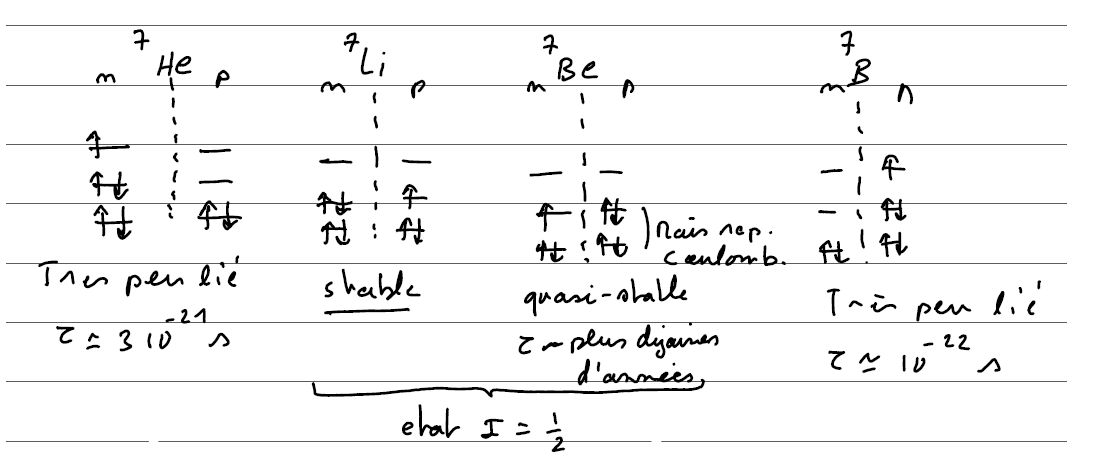
\includegraphics[scale=0.7]{Images4/A7.PNG}
    \caption{Différentes configurations d'isospin d'un noyau à $A = 7$}
    \label{fig:}
\end{figure}
On peut comprendre facilement par analogie avec la physique atomique que les isobares latéraux soient bien moins stables : les nucléons sont répartis dans des orbites bien plus élevées et sont donc moins liés, moins stables.

On s'aperçoit à nouveau que la symétrie sous échange de nucléons est brisée par la répulsion coulombienne. La configuration $^7B$ est légèrement plus instable que $^7He$, $^7Li$ est stable alors que $^7Be$ est quasi-stable avec un temps de vie de l'ordre de 10 ans. Ceci est uniquement du au fait que la différence entre l'énergie d'un état et son état miroir (c'est-à-dire deux états dont le nombre de protons de l'un est le nombre de neutrons de l'autre et vice-versa) provient uniquement de l'électromagnétisme.

\subsubsection{Modéliser le deuton : le potentiel créneau}


L'interaction entre nucléons provoque des états liés via le potentiel d'interaction que nous devons maintenant modéliser. Notre première approche est de considérer un potentiel en forme de puits sphérique $V(r)$. Nous devons encore définir la largeur et la profondeur de ce puits : de par les mesures de la section efficace, nous avons le rayon quadratique moyen $\sqrt{\expval{R^2}} = R_{RMS} = \SI{2.1}{fm}$. Nous avons également l'énergie expérimentale de liaison de l'état : $B = -2.2$[\si{MeV}]
\begin{figure}[H]
    \centering
    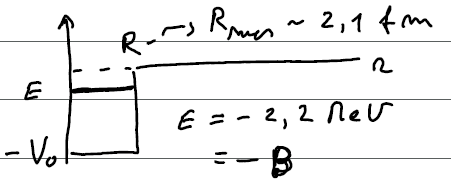
\includegraphics[scale=0.8]{Images4/Puits.PNG}
\end{figure}
A ce stade, nous choisissons un modèle presque jouet mais qui nous permettra de rendre compte d'un certain nombre de phénomènes non triviaux. Nous choisissons donc de modéliser $V(r)$ par une fonction créneau à $V_0$ de 0 à $R_{RMS}$. La question est donc de savoir s'il est possible d'obtenir une fonction d'onde d'énergie $B$ avec ce modèle et un rayon fixé au rayon expérimental. Le problème est identique au problème classique du puits de potentiel unidimensionnel fini bien connu. On rappelle donc l'expression de l'Hamiltonien :
\[
    -\dfrac{\hbar^2}{2\mu}\left(\nabla^2 + V(r)\right)\Psi \eq E\Psi
\]
\[
    \dfrac{1}{\mu} \eq \dfrac{1}{M_p} + \dfrac{1}{M_n} \; \approx \; \dfrac{2}{M_p}
\]
Via la séparation de variables $\Psi(r,\theta,\phi) \eq \chi(r)Y_l^m(\theta,\phi)$, avec $U(r) \eq r\chi(r)$ et en ignorant le terme de moment angulaire ($l=0$) :
\[
    -\dfrac{\hbar^2}{2\mu}\left(\ffdif{\chi(r)}{r} + \dfrac{2}{r}\fdif{chi(r)}{r}\right) + [V(r) + \dfrac{l(l+1)\hbar^2}{2\mu r^2}]\eq E\chi(r)
\]
\[
    -\dfrac{\hbar}{2\mu}\left(\ffdif{}{r} + V(r) \right)U(r) \eq EU(r)
\]
où $E<0$, V(r) le potentiel créneau défini précédemment.
Les solutions de cette équation sont :
\[
    \left\{
    \begin{array}{ll}
        r \;<\; R\; \longrightarrow \; U(r) \eq A \sin(k_1 r) + B \cos(k_1 r) \qquad \; \text{avec } k_1 \eq \sqrt{2m(E+V_0)}
    \\[7pt]
         r \;>\; R\; \longrightarrow \; U(r) \eq C e^{-k_2r} + D e^{k_2 r} \qquad \qquad \qquad \text{avec } k_2 \eq \sqrt{2mV_0}
    \end{array}
    \right.
\]
On étudie ensuite les conditions aux limites. De manière tout à fait classique, on impose que la fonction soit finie à l'infini pour conserver la propriété de carré sommable. On impose la continuité et la continuité des dérivées pour éviter les divergences. On impose également que la densité de probabilité soit finie (mais pas forcément nulle) en zéro. On obtient $B = 0$, $D = 0$ et le système suivant pour la continuité :
\[
    A \sin(k_1R) \eq Ce^{-k_2 R}
\]
\[
    k_1A\cos(k_1R) \eq -k_2 C e^{-k_2 R}
\]
On obtient de ces équations une relation trigonométrique transcendantale\footnote{Ca fait peur, je sais.}.
\[
    k_1 \cot(k_1R)  \eq -k_2
\]
Par leurs définitions, on tire également une relation entre $k_1$ et $k_2$.
\[
    k_1^2 + k_2^2 \eq 2mV_0
\]
On peut résoudre cette équation transcendantale par des moyens numériques ou graphiquement en écrivant $\cot(x) \approx 1 - x^2$ pour de petits x. Nous allons ici, supposer que $V_0 >> |E|$ et que donc $k_1 >> k_2$. Nous vérifierons à la fin de notre calcul si cette simplification était justifiée\footnote{Nous n'avons à ce stade aucune estimation de la profondeur du puits $V_0$.}.
\[
    \cot(k_1R) \; \approx \; 0
\]
\[
    K_1 R \eq \dfrac{\pi}{2}
\]
\[
    2mV_0 R^2 \eq \dfrac{\pi^2}{4}
\]
\[
    V_0 \eq \dfrac{\pi^2(\hbar c)^2}{4mR^2} \eq \dfrac{\pi^2 (198)^2}{4 939 (2.1)^2}
    \eq 25{MeV}
\]
On a toujours l'énergie expérimentale du système : $|B| = \SI{2.2}{MeV}$. On a donc que $V_0 \approx 10\cdot|B|$, l'approximation faite plus haut est donc bien valide.\\
En fin de compte nous avons donc, comme pour le puits de potentiel fini classique, une fonction sinus collée à une exponentielle. On a donc un effet tunnel permettant à la fonction d'onde du proton de se trouver en dehors de la zone de potentiel classiquement permise.
\begin{figure}[H]
    \centering
    \includegraphics[width=\textwidth]{Images4/ModèleDeuton.PNG}
\end{figure}
On note qu'il existe une probabilité de présence relativement élevée hors du rayon $R$. Il ne faut cependant pas oublier que la réelle partie radiale de la fonction d'onde est $\chi(r)$ et que donc le facteur $\dfrac{1}{r}$ atténue nettement cette probabilité.\\
On note aussi que pour un $V_0$ un peu moins profond, nous n'aurions pas d'état lié neutron-proton et nous vivrions dans un monde bien différent.\\

On calcule également l'intégrale de ce puits de potentiel sphérique, cette valeur nous servira de point d'appui\footnote{Elle sera considérée comme une donnée à reproduire.} pour le développement d'autres modèles de potentiel au Chapitre 18.
\[
    I 
    \eq \int V(r) \dif^3\vec{r} 
    \eq -4\pi\int_0^{\dfrac{R}{2}} V_0 r^2 \dif r 
    \eq -\dfrac{V_0}{8}\dfrac{4R^3}{3}
    \eq \SI{-170}{MeV \cdot fm^3}
\]
\subsubsection{Résolution de l'équation transcendante : Méthode 1}
\[
    -k_2 \eq k_1 \cot(k_1R)
\]
\[
    Z \eq \sqrt{\dfrac{E+V_0}{-E}} \left(= \dfrac{k_1}{k_2} \right)
\]
\[
    b \eq \sqrt{-2mE}R \simeq 0.23 R
\]
\[
    Z \eq -tan(bZ)
\]
On cherche donc les zéros de la fonction. 
\[
    f(Z) \eq Z + tan(bZ)
\]
On résout finalement en trouvant l'intersection de la fonction avec l'axe horizontal.
\begin{figure}[H]
    \centering
    \includegraphics[width=\textwidth]{Images4/graphe résolution graphique.PNG}
\end{figure}
\begin{figure}[H]
    \centering
    \includegraphics[width=\textwidth]{Images4/graphe résolution graphique 2.PNG}
\end{figure}
\subsubsection{Résolution de l'équation transcendante : Méthode 2}
On réécrit l'équation autrement.
\[
    x \eq k_1R
\]
\[
    y \eq k_2 R
\]
\[
    y \eq -x \cot(x) \simeq -x \left( \dfrac{1-\dfrac{x^2}{2}}{x} + \mathcal{O}(x^3) \right) \simeq \dfrac{x^2}{2} -1
\]
\[
    x^2 + y^2 \eq 2mV_0R^2 \; > \; \big(\dfrac{\pi}{2}\big)^2 \rightarrow car\ \cot(\dfrac{\pi}{2}) = 0
\]

L'inéquation est la condition pour avoir une solution à cette équation. On voit aussi graphiquement que pour des valeurs assez élevées pour le rayon du cercle, on peut avoir plusieurs solutions.
\begin{figure}[H]
    \centering
    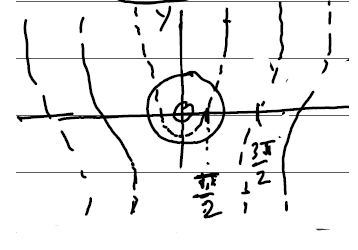
\includegraphics[scale=1.2]{Images4/EqTranscendante.PNG}
\end{figure}







\section{Les modèles macroscopiques : modèle de la goutte liquide}


Commençons par une série de réflexions sur les modèles microscopiques développés jusque ici. Ces modèles ne permettent pas encore de rendre compte clairement de l'énergie de liaison par nucléon (et non l'énergie totale!). Or, sur le graphe de cette quantité en fonction du nombre de masse $A$, au-delà du carbone, la valeur semble se stabiliser. Ce genre de comportement a probablement une origine physique que nous devons encore développer.\\ 
\begin{figure}[H]
    \centering
    \includegraphics[scale=1.0]{Images4/stabilité du fer.PNG}
\end{figure}
Le modèle en potentiel constant développé précédemment ne permet pas de rendre compte de l'imcompressibilité du noyau mesurée par le facteur de forme et la répartition de la charge que nous en avons extrait. En effet, il n'y a aucun potentiel répulsif ($>0$) pour empêcher que deux nucléons ne <<fusionnent>>.\\
\begin{figure}[H]
    \centering
    \includegraphics[width=\textwidth]{Images4/Modèle macro.PNG}
\end{figure}
L'objectif sera donc désormais de développer des modèles pouvant expliquer la répulsion entre nucléons ainsi que la stabilité de l'énergie par nucléon (qui sera considérée constante) au-delà du carbone.


\subsection{Hypothèses du modèle de la goutte liquide}


Le puit de potentiel présenté dans la section précédente ressemble traits pour traits à l'interaction de Van der Waals : interaction attractive à grande distance mais répulsive à très courte distance. C'est l'interaction qui est par exemple utilisée pour décrire une goutte d'eau. Nous allons donc supposer, de façon bien cavalière, que les nucléons dans le noyau ont un comportement semblable aux molécules d'eau dans une goutte : c'est le modèle de la goutte d'eau.\footnote{On voit bien que Thalès, qui pensait que toute la matière était faite d'eau, était un visionnaire} Ce modèle primitif permet d'obtenir quelques résultats intéressants mais a bien entendu été supplanté par d'autres modèles plus avancés depuis sa création.\\

Commençons par regarder l'hypothèse d'un \textbf{fluide nucléaire incompressible}. La forme de la distribution de charge établie à l'aide de la section efficace nous l'indique : le fait d'avoir un plateau central montre bien que même l'ajout d'un nucléon, sur la surface de la sphère qu'est le noyau, ne fait pas réduire de volume le coeur du noyau. Avec un liquide compressible on aurait eu une sorte de cloche avec un maximum au centre, les particules centrales se seraient compressées sous l'influence de celles de la surface.\\
\begin{figure}
    \centering
    \includegraphics{Images4/DensitéFinale.PNG}
\end{figure}
Rappelons quelques résultats et hypothèses qui nous seront utiles dans notre modèle:
\begin{itemize}
    \item la distance entre deux nucléons (qui est supposée constante dans tout le noyau car on utilise un modèle incompressible \textcolor{red}{demander au prof si c'est bon}) est $r_0 = \SI{1.2}{fm}$. Nous avions également obtenu que le rayon du noyau est $R=r_0A^{1/3}$

    \item Nous supposons dans notre modèle qu'un neutron occupe le même volume qu'un proton et que la probabilité de présence du neutron est constante sur tout le volume (cst en $r,\theta,\varphi$ pour $r<R$) et est la même que celle du proton. Dès lors :\textcolor{red}{Mais est-ce qu'on suppose pour autant qu'on a autant de protons que de neutrons?}
    $$ \rho_{nucleon} \eq 2 \rho_{charge} $$
    
    \item Nous avons aussi l'hypothèse (vérifiée expérimentalement!) que la force d'interaction nucléaire ne dépend pas de la charge des particules.
\end{itemize}


\subsection{Modéliser l'énergie de liaison grâce au modèle de la goutte liquide de Bohr}



Sur base de ces hypothèses et en rajoutant les interactions quantiques on obtient ce modèle pour l'énergie d'interaction\footnote{Définie comme l'opposé de l'énergie du système qui doit toujours être négative pour être un système lié.} :
\begin{equation}
\boxed{
    \quad B(A,Z) \quad\eq\quad
    \underbrace{a_V A}_{\text{Volumique}}
    \quad -\quad
    \underbrace{a_{surf} A^{2/3}}_{\text{Surfacique}}
    \quad-\quad
    \underbrace{a_c Z^2 A^{-1/3 }}_{Coulomb}
    \quad-\quad 
    \underbrace{a_{sym}\dfrac{(Z-N)^2}{A}}_{\text{Asymétrie}}
    \quad+\quad 
    \underbrace{\delta(A)}_{\text{Parité}}}\quad
    \label{B}
\end{equation}
Présentons brièvement chacun des termes présent dans l'équation de l'énergie d'interaction avant de les développer plus en détail:
\begin{itemize}[label = $\bullet$]
    \item \textbf{Volume} : décrit l'interaction forte entre les nucléons.
    
    \item \textbf{Surface} : Le terme de volume considère que tous les nucléons sont entourés de proches voisins, le terme vient donc réduire l'énergie proportionnellement à ces <<voisins manquants>> à la surface du noyau. On peut le voir comme un terme de tension superficielle.
    
    \item \textbf{Répulsion coulombienne} : Les protons du noyau se repoussent via la force de Coulomb (on a déjà observé les effets de cette interaction plus tôt). Le terme $A^{-1/3}$ est l'équivalent $\dfrac{1}{r}$ étant donné que $R=r_0A^{1/3}$.
    
    \item \textbf{Asymétrie} : Phénoménologiquement, on voit bien que les atomes qui présentent une  forte asymétrie dans leur nombre de protons et de neutons ne sont pas stables. On modélise ce comportement par cette expression, le carré indique bien que l'asymétrie diminue l'énergie d'interaction peu importe son "sens". Le facteur $\dfrac{1}{A}$ exprime le fait que le facteur d'asymétrie devienne de moins en moins influent au fur et à mesure que la masse des atomes augmente. En effet, dans les noyaux lourds, on voit beaucoup d'isotopes asymétriques stables.
    
    \item \textbf{Parité} : A nouveau, on remarque que la parité des nombres de nucléons intervient aussi dans l'énergie de liaison. Le cas le plus favorable est une configuration pair-pair, le cas <<classique>> est pair-impair et le cas défavorable impair-impair. Sur 274 atomes stables, 60.2\% sont pair-pair, 38.3\% pair-impair et 1.5\% sont impair-impair.\footnote{Source : notes de Buskulic. Le prof a donné les mauvais chiffres au cours}
\end{itemize}

\subsubsection{Développements des différents termes}
\paragraph{Développement pour le terme volumique :}


Le terme de volume décrit l'interaction attractive entre les nucléons due à la force nucléaire. Nous avons ainsi supposé que l'énergie de liaison entre deux nucléons est toujours la même : le terme volumique a ainsi la forme $a_{\text{volumique}} \cdot A$. Ainsi, connaissant l'énergie de liaison du deuton ($2.2 [\si{MeV}]$), nous avons que l'énergie de liaison par nucléon au sein du noyau est $1.1 [\si{MeV}]$. Nous avons modélisé le nucléon par une sphère : si nous supposons que les nucléons forment un empilement compact HC (Hexagonal Compact, cfr vos cours de cristallo), nous avons que chaque nucléon est entouré de 6 nucléons selon un plan, et de 3 nucléons au dessus (donc 3 également en dessous). Par conséquent, selon ces hypothèses, chaque nucléon est entouré de 12 autres nucléons avec lesquels il est lié avec une énergie de liaison de $1.1 [\si{MeV}]$ et l'énergie de liaison est donc $13.2 [\si{MeV}]$.\\

Cependant, nous avons fait l'hypothèse grossière que l'énergie de liaison du deuton était transposable dans un environnement nucléaire où la densité est plus élevée. De plus, nous n'avons pas tenu compte des effets de surface en supposant que chaque nucléon avait 12 voisins : nous n'avons pas encore pris en compte le fait que les nucléons à la surface avaient moins de voisins.


\paragraph{Développement pour le terme surfacique :}


Comme indiqué au paragraphe précédent, il y a eu un sur-comptage des liaisons entre nucléons : nous avons en surface moins de liaisons entre les nucléons. Ceci est analogue à la tension de surface (également appelée tension superficielle) qui maintient une goutte d'eau dans sa symétrie sphérique : elle veut minimiser sa surface en maximisant son volume (pour pouvoir minimiser son énergie totale), tout comme notre noyau.\\
Dès lors, le terme surfacique aura la forme $- a_{\text{Surfacique}} A^{2/3} $


\paragraph{Développement pour la répulsion coulombienne :}


Nous avons donc que tous les protons qui sont dans le noyau se repoussent suivant le potentiel de Coulomb : ceci tend à diminuer l'énergie de liaison du noyau. Puisque le potentiel de coulomb est proportionnel au produit des charges divisé par le rayon, nous avons bien que le terme de \textbf{répulsion coulombienne} est décrit par $-a_{\text{Coulomb}} Z^2 A^{-1/3}$.\\

Pour obtenir la valeur du coefficient $a_{\text{Coulomb}}$, nous devons juste calculer le travail (donc l'énergie) nécessaire pour amener tous les protons dans cette sphère. Pour faciliter le calcul, nous considérons un modèle continu dans lequel nous devons créer une sphère (= le noyau) uniformément chargée. Nous considérons donc que nous disposons déjà d'une très petite ($r \rightarrow 0$) sphère continue à laquelle nous ajoutons successivement des épaisseurs infinitésimales $dr$ jusqu'à arriver à une sphère de rayon R. Ainsi, le travail $dW$ nécessaire pour ajouter une coquille d'épaisseur infinitésimale $dr$, de charge $dq$, à la sphère déjà existante est:
\begin{align*}
    dW(r) &\eq 
    dq \cdot V(r) \qquad \qquad \quad \;\text{avec $V(r)$ le potentiel créé par la sphère déjà existante}
    \\ 
    &\eq 
    \rho 4\pi r^2 \dif r \cdot \dfrac{ \rho \dfrac{4}{3}\pi r^3}{4\pi\epsilon_0 r}
    \qquad \text{avec } \rho \eq \dfrac{Ze}{\dfrac{4}{3}\pi R^3}\text{ : la densité est constante dans le volume}\\
    &\eq
    \dfrac{4\pi}{3\epsilon_0}\rho^2 r^4 \dif r \\
    \Leftrightarrow \qquad W &\eq
    \int_0^R dW \eq \dfrac{3}{5}\underbrace{\dfrac{e^2}{4\pi\epsilon_0}}_{\alpha}\dfrac{Z^2}{r_0}A^{-1/3}
\end{align*}

On obtient donc le coefficient du terme de Coulomb, $a_{\text{Coulomb}}$, avec $\hbar c \approx \SI{198}{MeV \cdot fm}$.
\[
    a_c \eq \dfrac{3}{5}\dfrac{\alpha}{r_0} \hbar c \approx \SI{0.72}{MeV}
\]
On considère que ce résultat est assez précis dans la limite où l'approximation continue du noyau par une sphère continue uniformément chargée est correcte. Dès lors, pour des A peu élevés, ce modèle n'est plus valable et il faut faire un calcul avec l'ajout de charges discrètes.


\paragraph{Discussion autour du terme d'asymétrie :} 


Prenons l'exemple du système avec $A = 12$ ($^{12}C$ par exemple). Par le principe d'exclusion de Pauli, chaque niveau d'énergie peut être occupé par deux nucléons identiques de spins différents et donc un même niveau par 4 nucléons (2 protons, 2 neutrons) pour autant que nous négligeons la répulsion coulombienne.\\
On définit également $\Delta E$, la différence d'énergie entre deux états d'énergie consécutifs. Nous faisons l'hypothèse que $\Delta E$ est constant, ce qui est une grosse approximation. En effet, il semble peut probable que cette différence soit constante lorsqu'on monte en énergie (pensez aux électrons dans les atomes où la différence entre deux niveaux varie en fonction de n).\\
\begin{figure}[ht]
    \centering
    \includegraphics[scale = 0.7]{Images4/tableau_Asymétrie.PNG}
\end{figure}
La fonction $\dfrac{(N-Z)^2}{A}$ n'est donc qu'une approximation des résultats présentés dans le tableau. On obtient donc $a_{sym}$.
\[
    a_{\text{asymétrique}} \eq \dfrac{A\Delta E}{8}
\]
Nous pouvons faire deux remarques sur nos développements:
\begin{itemize}
    \item Dans le tableau, on a supposé que les états d'énergie entre protons et neutrons étaient identiques alors que, en pratique, ceux des protons sont plus élevés que ceux des neutrons. Cependant, cette fois-ci, nous devons les considérer identiques car nous avons déjà tenu compte de la répulsion coulombienne dans le terme coulombien!
    \item Nous avons également fait la supposition que, par état, la dégénérescence était de 4 (un état d'énergie peut contenir 2 protons de spin opposé et 2 neutrons de spin opposés) alors qu'en pratique, il faut regarder les nombres quantiques (comme nous devons regarder les nombres quantiques dans les atomes pour voir le nombre maximum d'électrons que nous pouvons mettre par niveau $n$).
\end{itemize}

\paragraph{Détail du terme d'appariement :} 


Le terme d'appariement est une correction purement empirique basée sur l'observation de <<nombres magiques>>\footnote{A notre niveau du moins} permettant une meilleure stabilité des atomes. La base de ces constatations est une meilleure stabilité des noyaux pair-pair (qui ont une nombre pair de proton et un nombre pair de neutrons).\\
\begin{figure}[ht]
    \centering
    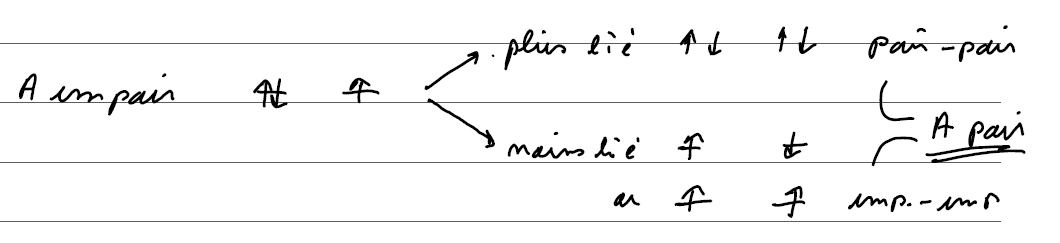
\includegraphics[width=\textwidth]{Images4/appariement.PNG}
\end{figure}

Nous supposons donc un mécanisme, une force d'appariement (dont on n'explique pas encore l'origine physique!), qui fait qu'un état est plus lié quand les couches du noyau sont pleines que lorsqu'elles sont vides \textcolor{red}{Pourquoi on parle de couches ici, vu qu'on n'est pas dans le modèle en couche mais dans le modèle de la goutte liquide...est-ce que par couche il ne faudrait pas plutôt dire <<niveau>>? Ca me semblerait déjà mieux}. Ainsi, le terme d'appariement est totalement empirique.\\
\begin{figure}[htp]
    \centering
    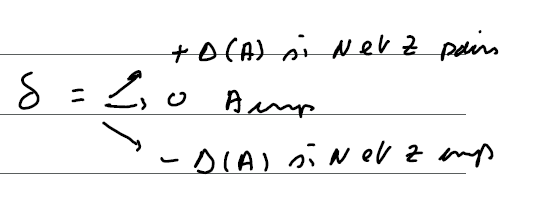
\includegraphics{Images4/appariement2.PNG}
\end{figure}
\[
    a_p \; \approx \; \SI{12}{MeV}
\]



\subsubsection{Comment varie $\Delta E$ en fonction de $A$ ?} 


On modélise la variation de $\Delta E$ à partir du comportement d'une particule quantique dans un puits de potentiel\footnote{Ce n'est pas exactement le développement fait par le prof en cours. On y a rajouté des étapes/coefficients qui nous semblaient plus corrects.}.\\
\[
    \dfrac{\hbar^2}{2\mu}\nabla^2 \psi \eq (E- V_0)\psi
\]
Pour un puits fini en 3D, on a comme solution de ce problème aux valeurs propres:
\begin{align*}
    \psi &\;\propto\; 
    \Pi_i \sin(k_i x_i) \qquad \text{avec }\; i ={x,y,z}\\
    E &\eq \dfrac{\hbar^2 k^2}{2m}
\end{align*}
Comme on a un système constitué de deux corps en interaction dans un potentiel central (coordonnées sphériques), la largeur du puits de potentiel $a$ doit satisfaire : $a = 2R$. On introduit ensuite des conditions limites au système en imposant qu'il s'annule en $a$.
\[
    ak_i \eq n_i \pi
\]
\[
    k^2 \eq k_x^2 + k_y^2 + k_z^2 \eq \dfrac{n^2\pi^2}{a^2}
\]
Et on obtient finalement une expression pour $\Delta E$ en fonction de $A$\footnote{Pour le facteur $\gamma,$ voir les discussions liées à la densité de charge.}.
\[
    \dfrac{|\Delta E|}{\Delta a} 
    \eq \dfrac{\partial E}{\partial a}\Delta a
    \eq \dfrac{\partial}{\partial a}\left( \dfrac{\hbar^2n^2\pi^2}{2ma^2}\right)\underbrace{\Delta a}_{=\Delta(2R)= 2*\gamma\approx \SI{5}{fm}}
\]
\[
    a^3 \eq 8r_0^3 A
\]
\[
    r_0 \eq \SI{1.2}{fm}
\]
\[
    \Delta E \eq a_{sym} \;\approx\; \dfrac{150}{A}\si{MeV}
\]
Cette valeur est en excellent accord avec les mesures expérimentales : en fait on a eu "trop" de chances parce que nos approximations sont excessives mais le résultat est +- correct.





\subsection{Formule de masse de Bethe-Weizsäcker}


\begin{figure}[ht]
    \centering
    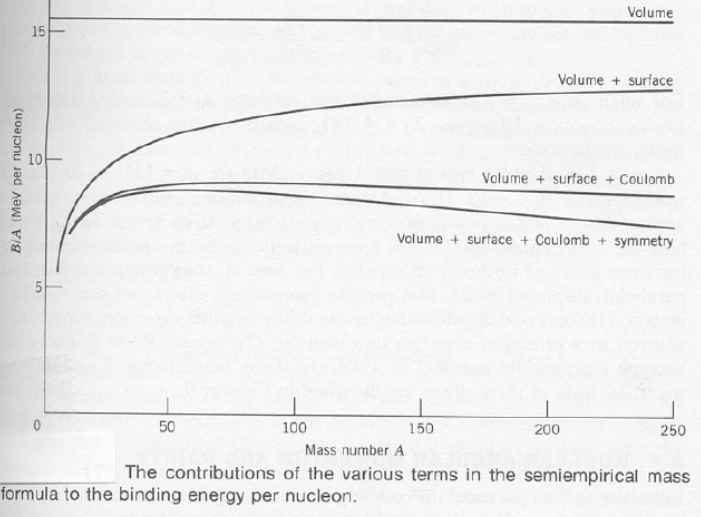
\includegraphics{Images4/correction.PNG}
    \caption{Énergie de liaison en fonction de $A$, pour différents cas}
\end{figure}
On présente ici les différentes corrections en fonction du nombre de masse A. On voit que le terme de répulsion coulombienne et le terme surfacique dominent largement les corrections.\\
Le modèle de la goutte d'eau représente les effets ayant un équivalent classique : effet volumique, effet surfacique\footnote{L'interaction forte n'a bien entendu aucun équivalent classique mais on peut l'apparenter à la force de van der Waals dans les gouttes d'eau.} et la répulsion coulombienne. On ajoute ensuite à ce modèle deux corrections de ressort purement quantique, les termes de symétrie et d'appariement, qui ne prennent d'importance que lorsque $A$ est grand.\\

Connaissant l'énergie de liaison atomique $B(A,Z)$ de par notre modèle de la goutte liquide, il ne reste plus qu'à soustraire à la masse des constituants du noyau cette énergie pour obtenir la masse réelle du noyau.\\

\begin{figure}[ht]
    \centering
    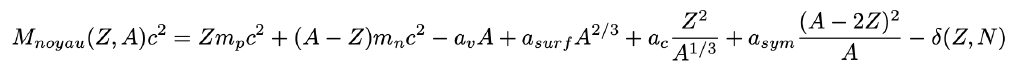
\includegraphics[width=\textwidth] {Images4/Bethe.PNG}
\end{figure}
Nous l'avons dit, il existe des nombres <<magiques>> de nucléons par noyau qui lui octroient une meilleure stabilité. Leur existence laisse supposer une structure en couche, tout comme les gaz rares possèdent une plus haute stabilité car leur structure en couche est fermée et est donc composée de nombres bien particuliers d'électrons.


\subsection{La vallée de stabilité}


Pour déterminer la vallée de stabilité des atomes (= ensemble des couples $(Z,N)$ ou $(Z,A)$ dont les noyaux sont stables), il suffit de minimiser la masse d'un atome $M_{at}(Z,A)$ ou encore de maximiser son énergie de liaison $B(Z,A)$\footnote{En prenant comme hypothèse que $m_p \approx m_n$} pour un $A$ donné.
\[
    \dfrac{\p M_{at}}{\p Z} \eq 0
\]
En prenant B comme l'énergie de liaison nucléaire et en négligeant l'énergie de liaison atomique:
\[
    \dfrac{\partial}{\partial Z}\left(Zm_p + Zm_e + (A-Z)m_n -B(A,Z)\right) 
    \eq \underbrace{m_p + m_e - m_n}_{\approx 0} + \dfrac{\partial B}{\partial Z}
    \eq 0
\]
\[
    \dfrac{a_c}{2a_{sym}}Z A^{2/3} - A + 2Z \eq 0
\]
\[
    \boxed{\quad
        Z \eq \dfrac{A}{2} \dfrac{1}{1 + \dfrac{a_{coulomb}}{4a_{sym}}A^{2/3}}\quad
    }
\]
\begin{figure}[H]
    \centering
    \includegraphics[scale =1.5] {Images4/Vallée.PNG}
    \caption{Comparaison entre la vallée de stabilité des atomes et la droite Z=N}
    \label{vallee}
\end{figure}
\begin{figure}[H]
    \centering
    \includegraphics[scale =1.0] {Images4/Graphe_Décomposition.PNG}
    \caption{Courbes d'énergie pour des états isobares}
    \label{decomp_noyau}
\end{figure}
On peut maintenant considérer une coupe isobarique du graphe \ref{vallee}, c'est-à dire regarder la variation en énergie des différents isobares. C'est ce qui est présenté dans le superbe Pollock \ref{decomp_noyau}. On peut voir que la stabilité se trouve autour de la symétrie en neutrons et protons.\\

Tout d'abord, on a séparé en deux cas distincts : A est impair à gauche et pair à droite. On voit donc sur le graphe de droite deux courbes dont l'une semble simplement décalée d'une valeur constante par rapport à l'autre. La courbe du bas est la courbe correspondant à des structures pair-pair et celles du dessus impair-impair. Pour A impair, il n'y a bien entendu par de distinction à faire : nous n'avons qu'un seule courbe.\\

Les flèches représentées indiquent les transitions entre noyau, elles ont donc toujours une orientation descendantes, elles vont vers l'état de moindre énergie. Ces désintégration se font via l'émission de rayonnement $\beta^+$ si un proton se désintègre en un neutron, un positron et un neutrino et via un rayonnement $\beta^-$ si un neutron se dissocie en un proton, un électron et un antineutrino. Il peut bien entendu également y avoir des désintégrations $\beta$ dans le graphe de gauche, les flèches ne sont simplement pas représentées.








\section{De l'interaction nucléon-nucléon au potentiel moyen de Wood-Saxon}
\subsection{Potentiel de Yukawa}


La démarche ici est tout à fait comparable au modèle Hartree-Fock de la physique atomique. On va passer d'une interaction entre deux éléments à un potentiel moyen régnant dans le noyau. Ce faisant, nous pourrons obtenir les nombres quantiques associés au système. Le modèle ne sera bien entendu pas exact pour autant et bon nombre d'approximations seront faites.\\

Dans un cas concret, on se retrouve face à un problème similaire à celui de la partie atomique du cours : pour déterminer la densité du noyau, nous avons besoin des fonctions d'onde et vice-versa. L'utilisation de méthodes itératives est donc nécessaire.\footnote{On peut se souvenir du potentiel non-local dans l'équation d'Hartree-Fock qui donne lieu à une équation intégro-différentielle que l'on résout à l'aide de la méthode SCF, une méthode itérative.} La résolution concrète de ces équations n'est pas le sujet du cours.\\

Nous allons développer le modèle de Yukawa dans le cas du deuton à l'aide d'une série de mesures et de constatations effectuées plus tôt dans le cadre du modèle potentiel carré\footnote{NB : le choix d'un potentiel quadratique correspondant à l'oscillateur harmonique aurait été tout autant valable, il nous fallait seulement un potentiel simple permettant d'aboutir à une solution analytique.}. Ainsi, nous connaissons les valeurs suivantes du problème du deuton :
\[
    R \eq |\Vec{r_n} - \Vec{r_p}| \eq \SI{2.1}{fm}
\]
\[
    E \eq -B \eq \SI{-2.2}{MeV}
\]
\[
    V_0 \eq \SI{35}{MeV}
\]
\[
    I \eq \int_V V_{NN}d\vec{r}^3 \eq \SI{-170}{MeV \cdot fm^3}
\]
Le potentiel carré présente deux problèmes évidents :
\begin{itemize}[label = $\bullet$]
    \item Il ne permet pas de rendre compte de la répulsion entre nucléons pour de très petites distances. On voudrait donc introduire une divergence positive du potentiel quand on approche 0.
    \item Il ne rend pas compte de la douceur de la chute de la densité quand on dépasse le rayon du noyau. On impose donc une décroissance exponentielle en dehors du noyau.
\end{itemize}
On obtient ce potentiel dit de Yukawa :
\begin{figure}[H]
    \centering
    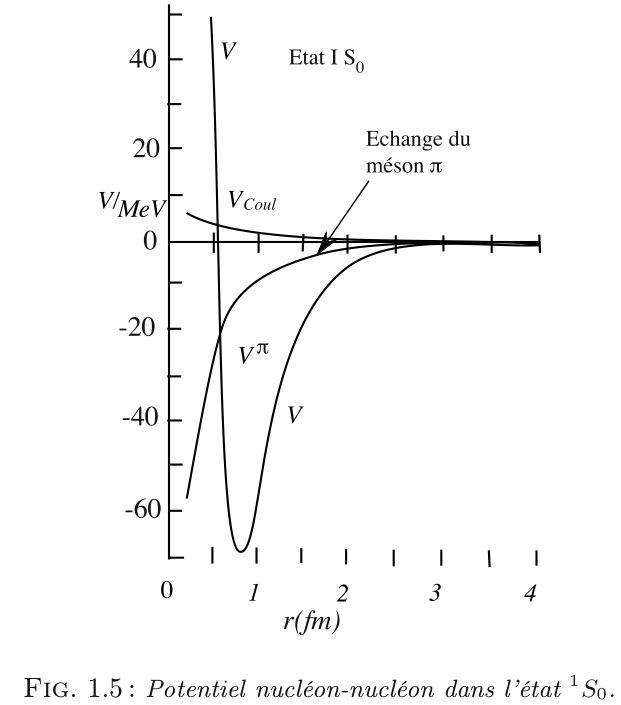
\includegraphics[scale =0.42] {Images4/Potentiel_Yukawa.jpg}
\end{figure}
Formellement, on a atténué exponentiellement l'équivalent d'un potentiel coulombien, en $\dfrac{1}{r}$. On introduit plusieurs grandeurs :
\begin{itemize}[label = $\bullet$]
    \item $\dfrac{g^2}{4\pi}$ Bien entendu le facteur $4\pi$ n'a pas d'intérêt en soi, il nous servira juste à comparer proprement les amplitudes des constantes de couplage $g$ et $e$. Notons d'ailleurs qu'identifier $g$ à une charge électrique est une hérésie, il ne s'agit pas de l'interaction coulombienne. Nous sommes dans une démarche d'analogie et de comparaison.
    \item $\lambda$ a les dimensions d'une longueur : il s'agit de la longueur d'atténuation du potentiel. $\lambda$ apparaîtra dans un terme $e^{-\dfrac{(r-r_0)}{\lambda}}$.
    \item $r_0$ est le rayon d'équilibre d'un état stationnaire de la particule dans le potentiel. Il s'agit du rayon auquel l'exponentielle prend le pas sur le potentiel coulombien (quand $r<r_0$). $r_0 \approx [0.1;0.5]$\si{fm}
\end{itemize}
Nous modéliserons ainsi le potentiel d'interaction entre nucléons $U(r)$ (rendant seulement compte de l'interaction forte) comme:\footnote{Cette écriture est assez générale pour les interactions, il suffit de moduler les paramètres libres.}
\[
\boxed{
    U(r) \eq -\dfrac{g^2}{4\pi} \dfrac{1}{r}e^{-(r-r_0)/\lambda}
    }
\]
On impose la conservation de l'intégrale sur le volume, nommée $I$ et valant \SI{170}{MeV \cdot fm^3}. Par ce biais, on va pouvoir imposer une gamme de valeur pour $\lambda$ en faisant varier g sur l'intervalle $[e,1]$ où $e$ représente un couplage infinitésimal (électromagnétisme) et 1 un très grand couplage. On définit également $\alpha_s = \dfrac{g^2}{4\pi}$ la constante adimensionnelle de structure du système par analogie avec la constante de structure fine $\alpha$.
\begin{align*}
    \dfrac{I}{\hbar c}  
    \;\equiv\; \int U \; d^3\Vec{r}
    &\eq \alpha_s \int_S \dfrac{1}{r}e^{-(r-r_0)/\lambda} d^3\Vec{r}\\
    &\eq 4\pi \alpha_s \int_{r_0}^\infty \dfrac{1}{r}e^{-(r-r_0)/\lambda} r^2 \dif r\\
    &\eq 4\pi\alpha_s e^{r_0/\lambda} \int_{r_0}^\infty e^{-r/\lambda} r \dif r
\end{align*}
\begin{align*}
    \int_{r_0}^\infty re^{-r/\lambda} &\eq [-\lambda r e^{-r/\lambda}]_{r_0}^\infty + \lambda\int_{r_0}^\infty e^{-r/\lambda}dr\\
    &\eq \lambda r_0 e^{-r_0/\lambda} + \lambda (-\lambda)[e^{-r/\lambda}]_{r_0}^\infty\\
    &\eq \lambda e^{-r_0/\lambda}(r_0 + \lambda)
\end{align*}
\[
    \boxed{
        \dfrac{I} {\hbar c}\eq 4\pi \alpha_s \lambda(\lambda + r_0)
        \eq g^2\lambda(\lambda + r_0)}
\]
\[
    \lambda \eq \dfrac{-r_0 \pm \sqrt{r_0^2 + \dfrac{I}{\pi\alpha_s\hbar c}}}{2}
\]
Nous obtenons ainsi deux valeurs de la longueur d'atténuation $\lambda$. Dans l'intérêt de la simplicité de la discussion, on fixe $r_0$ à 0 car il en est déjà très proche, physiquement parlant cela revient à dire que l'exponentielle liée au méson ne prend le pas sur le potentiel coulombien qu'en r = 0, c'est un petit peu délicat à justifier mais ça n'est pas insensé. On ne considère également que la valeur positive de $\lambda$ car une longueur négative n'a pas de sens physique. En remplaçant ainsi $I$ par sa valeur (\SI{170}{MeV \cdot fm^3}) et $\alpha_s$ par son intervalle possible $[e,1]$ où e désigne la charge élémentaire dans le système d'unités naturelles : $\hbar = c = \epsilon_0 = 1$ où\footnote{Il suffit de remplacer dans l'expression de la constante de structure fine $\alpha \eq \dfrac{e^2}{4\pi\epsilon_0 \hbar c}$} $e \approx 0.3$. On peut enfin obtenir un intervalle pour $\lambda$ :
\[
    \lambda \eq \dfrac{1}{2} \sqrt{\dfrac{I}{\pi\alpha_s\hbar c}}
    \quad \Rightarrow \quad
    \lambda \;\in\; [3;0.9]\; \si{fm}
\]

Cet intervalle a donc été obtenu en supposant une profondeur du puits de potentiel similaire à la profondeur permettant d'expliquer l'énergie de liaison du deuton : nous avons utilisé $I=170$.\\

C'est ici que la discussion devient vraiment intéressante. Nous avons donc un intervalle de valeur, dépendant de l'intensité du couplage, pour la longueur d'atténuation $\lambda$ du potentiel moyen. Par une analyse dimensionnelle, et en utilisant les constantes fondamentales associées, on peut transformer cette longueur en une masse (en unités naturelles, [L]=[M$^{-1}$]).\footnote{En continuant cette analogie avec l'électromagnétisme, on peut arriver à une conclusion très intéressante. Pour retrouver l'interaction électromagnétique classique, il nous suffit de remplacer g par e et... de poser $m = 0$, ce qui supposerait une particule médiatrice de l'interaction de masse nulle comme... le photon hé oui ! Dès lors, $\lambda$ serait l'équivalent de la longueur d'onde du photon.}\\
L'hypothèse de Yukawa consiste à supposer que cette masse est associée à une particule.\footnote{Si nous comprenons la longueur d'atténuation du potentiel de Yukawa comme la longueur d'onde d'un méson, nous obtenons via $\lambda \eq \dfrac{\hbar c}{mc^2}$ que $P=mc$ : ainsi le méson se déplacerait à la vitesse de la lumière? Ceci est peut être possible si on considère des particules virtuelles \textcolor{red}{question pour le prof : le méson irait à la vitesse de la lumière? Parce que le passage d'une unité atomique de longueur à une unité atomique de masse semble impliquer cela.}}\\
\[
    \lambda \eq \dfrac{\hbar c}{mc^2}
\]
\[
    e^{-r/\lambda} \eq e^{-mr} \qquad \text{car } \lambda \eq \dfrac{\hbar c}{mc^2} \eq \dfrac{1\cdot 1}{m \cdot 1^2} \eq \dfrac{1}{m}
\]
Il peut sembler étonnant de remplacer une longueur par une masse : en fait, puisque nous somme en unités atomiques, nous avons que l'unité de longueur est équivalente à une unité de masse$^{-1}$.
\[
    m\;\in\; [65:215]\si{MeV}
\]


\subsection{L'hypothèse de Yukawa et le pion}



La particule dont l'existence est supposée par Yukawa existe bel et bien, se nomme le pion, de la famille des mésons. C'est donc cette particule qui est à l'origine de l'atténuation exponentielle du potentiel de l'interaction entre deux nucléons. Sa masse est de \SI{140}{MeV}, ce qui correspond au milieu de l'intervalle déterminé. On peut donc en déduire une longueur d'onde et une constante de structure. Notons bien qu'à ce stade nous n'avons pas encore su introduire la remontée exponentielle du potentiel vers $r=0$, nous pourrons le faire en introduisant une autre nouvelle particule plus tard dans notre discussion.
\[
    m_\pi \eq \SI{140}{MeV} \quad \longrightarrow \quad \lambda \eq \SI{1.4}{fm}\;;\;\alpha_s \eq 0.035\;;\; g^2\eq 0.44
\]
%Le prof s'est planté dans les slides, il avait écrit g = 0.44 mais ça ne colle pas avec la valeur de 0.035 tandis que g^2 = 0.44 oui
L'ordre de grandeur du couplage nucléaire ($\alpha_s$ = 0.035) est un petit ordre de grandeur supérieur au couplage électromagnétique ($\alpha_{EM} \approx 1/137 \approx 0.007$). Aussi, $g^2$ est suffisamment petit (0.44$<$1) pour pouvoir utiliser la théorie des perturbations.\\

Nous avons donc obtenu $g$ en supposant un potentiel d'interaction entre nucléons semblable au potentiel EM, avec cependant un terme d'atténuation exponentielle. Notre interaction avait trois paramètres libres : $r_0, \lambda, g$. Nous avons pu obtenir les valeurs de ces paramètres en suivant les étapes suivantes:
\begin{enumerate}
    \item $r_0$ est négligé (=0) : il ne nous reste que 2 paramètres à fixer.
    
    \item On fixe la valeur de l'intégrale du potentiel à \SI{170}{MeV \cdot fm^3}, c'est-à-dire à la valeur de l'intégrale du potentiel carré qui nous avait permis d'obtenir des états liés pour le deuton. Nous avons alors une relation pour deux inconnues ($\lambda$ et $g$).
    
    \item Nous identifions le pion, de masse \SI{140}{MeV}, comme responsable de l'interaction. Nous avons alors une deuxième relation et nous pouvons déterminer les valeurs de $\lambda$ et $g$.\\
\end{enumerate}


\textbf{A ce stade, nous connaissons donc deux caractéristiques de l'interaction forte : son couplage $\alpha_s > \alpha$ d'un facteur 5 (en réalité il y a un facteur $10$) et sa portée qui est très courte $\lambda \approx 1$fm.}\\
L'hypothèse de Yukawa donne donc un sens physique à $m$ (ou, de façon équivalente, à $\lambda$) en l'associant à la masse d'une particule (pour $\lambda$ à la longueur d'onde de cette particule allant à vitesse $c$ \textcolor{red}{A verifier}). Jusqu'ici, nous n'avons illustré cette hypothèse que dans le cas d'états liés (dans un noyau). Cependant, si ce potentiel est effectivement celui décrivant l'interaction entre nucléons, notre modèle devrait permettre d'expliquer la diffusions de nucléons (collision de deux nucléons).\\

Avant de nous attaquer au potentiel de Yukawa et à ses implications, concentrons-nous d'abord sur ce que nous savons de l'électromagnétisme. Introduisons donc le potentiel scalaire électromagnétique $\Psi$.
\[
    \Psi \eq \dfrac{e}{4\pi \epsilon_0 r}(\hbar c)
\]
\[
    U \eq  \dfrac{\alpha}{r}(\hbar c)\eq e\Psi 
\]
$\Psi$ a les propriétés d'une onde et satisfait donc les équations suivantes\footnote{Attention l'opérateur $\nabla$ s'exprime dans les coordonnées sphériques.} :
\[
    \nabla^2 \Psi(\Vec{x}) \eq 0 \; \text{(équation de Laplace)}
\]
\[
    \Psi(\Vec{x}) \; \text{est une approximation statique de }\; \Phi(\Vec{x},t)
\]
\[
    \nabla^2 \Phi(\Vec{x},t) - \dfrac{\partial^2\Phi(\Vec{x},t)}{ \partial t^2} \eq 0 \; \text{(équation d'onde)}
\]
$\Psi$ représente donc une onde qui se déplace, on peut donc par l'hypothèse de Yukawa lui associer une particule. Quelles sont les équations que doit satisfaire cette particule? On commence par réexprimer les opérateurs énergie et quantité de mouvement au sens quantique.
\[
    E \eq\imag\hbar \dfrac{\partial}{\partial t}
\]
\[
    P\eq -i\hbar \nabla_r
\]
On peut donc réexprimer l'équation d'onde comme suit :
\[
    E^2 - P^2 \eq 0
\]
En identifiant cette formule à la formule relativiste de l'énergie, nous remarquons que la particule satisfaisant cette équation doit avoir une masse nulle : la photon. Ainsi, l'hypothèse de Yukawa permet d'associer à l'interaction électromagnétique un photon. Ce résultat est connu et nous indique que nous somme sur la bonne voie : Yukawa ne détruit pas la physique que nous connaissons!\\

On applique le même raisonnement pour l'interaction forte. Il s'agit à nouveau de trouver les équations qui gouvernent le comportement de notre méson (dont l'existence n'est encore qu'une hypothèse pour nous) pour en apprendre plus sur lui. On écrit $V_{NN}$ au sens d'une énergie potentielle liée à un potentiel scalaire $\Psi_s$.
\[
    V_{NN} \eq g\Psi_s
\]
\[
    \Psi_s \eq \dfrac{g}{4\pi\epsilon_0}\dfrac{1}{r}e^{-mr}
\]
On rappelle l'expression de nabla en coordonnées sphériques (puisque notre système est à symétrie sphérique, la partie angulaire du laplacien - qui concerne les $Y^m_l$ - sur la fonction sera nulle). $\Psi$ est donc solution de l'équation suivante, après avoir fait quelques dérivées triviales :
\[
    \nabla^2\Psi_s(r) 
    \eq \dfrac{1}{r^2}\dfrac{\partial^2}{\partial r^2}\left(r^2 \Psi_s\right)
    \eq m^2 \Psi_s
\]
\[
    \boxed{
        \nabla^2 \Psi_s - m^2\Psi_s \eq 0
    }
\]

On \textbf{suppose} en plus que, comme pour le cas de l'électromagnétisme, $\Psi_s(\Vec{x})$ est une approximation statique de $\Psi_s(\Vec{x},t)$. Il satisfait \textbf{l'équation de Klein-Gordon}.
\[
    \boxed{
        \nabla^2\Psi_s - \dfrac{\partial^2\Psi_s}{\partial t^2} \eq m^2 \Psi_s
    }
\]
En introduisant les opérateurs quantiques d'énergie et de quantité de mouvement :
\[
    E^2 - P^2 \eq m^2
\]
Ce qui correspond bien à l'expression relativiste caractérisant une particule de masse $m$. On associe donc une particule, le \textbf{pion}, au potentiel statique de l'interaction forte. Il appartient à la famille des mésons\footnote{Petit intermède éthymologique : méson vient du grec \emph{mesos} qui signifie milieu, car les mésons sont plus lourds que les leptons, mais plus légers que les baryons.} évoquée plus tôt. Jusqu'ici nous n'avons fait qu'un raisonnement abstrait (et par ailleurs peu rigoureux) : il nous faut maintenant vérifier nos prédictions osées par l'expérience.\\



\subsection{Preuves expérimentales de l'existence du pion}



On va donc créer des interactions fortes entre particules dans le continuum. A priori, le plus simple est d'utiliser des protons et des neutrons par leur facilité de production et leur stabilité. Il reste à choisir qui servira de cible et de projectile. Nous avons donc les quatre possibilités suivantes, les indices `c' et `p' désignant respectivement la cible et le projectile :
\begin{itemize}
    \item $n_p\; +\; n_c\; \longrightarrow\; n_p\;+\; n_c$ est à exclure au premier abord (cela sera fait, mais on n'en parle pas dans ce cours) car les neutrons sont instables : ils ne font donc pas une bonne cible.
    \item $p_p\; +\; n_c\; \longrightarrow\; p_p \;+\; n_c$ est également à exclure car, encore une fois, les neutrons ne font pas de bonnes cibles.
    \item $p_p\; +\; p_c\; \longrightarrow\; p_p \;+\; p_c$ est faisable (les protons sont stables) mais il y a une contamination électromagnétique dans l'interaction : cela complique nos mesures!
    \item $n_p\; +\; p_c\; \longrightarrow\; n_p \;+\; p_c$ est l'interaction la plus aisée à effectuer et ne comporte pas de contamination électromagnétique : c'est donc la diffusion des neutrons sur des protons cibles qui sera étudiée.
\end{itemize}
On travaille dans le référentiel centre de masse du système à deux corps (cfr. figure \ref{collision_np_yukawa}). Puisque nous supposons que nos deux corps ont la même masse, dans le référentiel CM, ils auront la même vitesse (au signe près). Cela revient entre autre à placer notre observateur au milieu des deux particules : $v_p = -v_n = -\dfrac{1}{2}v_{n,lab}$. Les angles de diffusion seront également différent du référentiel du laboratoire. On y réécrit donc la conservation de l'énergie :
\[
    E_0 \eq E_1 + E_2 \eq E_3 + E_4
\]
\begin{figure}[H]
    \centering
    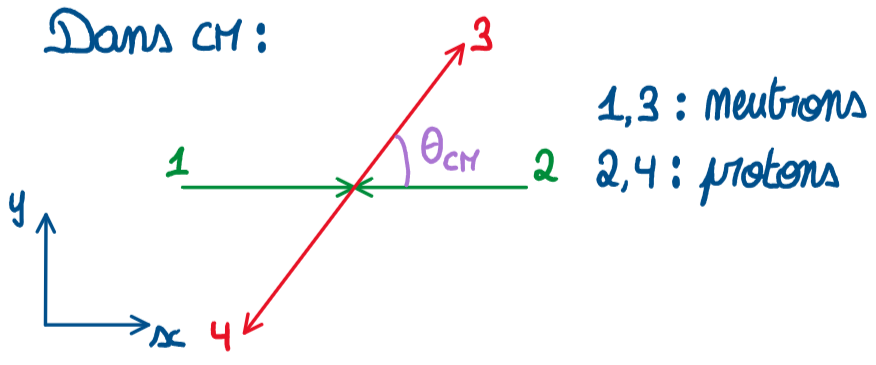
\includegraphics[scale = 0.6]{Images4/collision_CM.png}
    \caption{Visualisation de la collision dans le centre de masse}
    \label{collision_np_yukawa}
\end{figure}
Tout comme nous avons utilisé la notion de section efficace différentielle pour sonder l'interaction électromagnétique du noyau avec des particules $\alpha$, nous allons utiliser cette notion pour étudier le comportement de l'interaction forte entre le proton et le neutron lors de la collision. Les raisonnements faits pour l'étude du noyau sont toujours valables, aux constantes près qui varient mais, dans ce cours, on ne va faire que des relations de proportionnalité car seul un terme nous intéresse dans la section efficace. On écrit donc :
\[
    \fdif{\sigma}{\Omega}\Big|_{CM} \; \propto \; |T_{fi}(1+2\longrightarrow3+4)|^2
\]
\[
    T_{fi}(1+2\longrightarrow3+4)\; \propto \; \alpha_s \int \dfrac{1}{r}e^{-mr}e^{\imag\vec{q}\cdot\Vec{r}}d\Vec{r}^{\ 3}
    \qquad \text{où }\Vec{q} \eq \Vec{P_1} - \Vec{P_3}
\]
Cette intégrale est, à quelques facteurs près, strictement égale à celle résolue à la section \ref{calcul_Tfi} pour la diffusion de particule avec interaction électromagnétique. En utilisant ce résultat, nous obtenons :
\begin{align*}
    \int \dfrac{1}{r}e^{\imag\vec{q}\cdot\Vec{r}}e^{-\epsilon r} \;\;d^3\Vec{r}
    &\;\propto\; 
    \dfrac{4\pi\hbar^2}{q^2}\dfrac{1}{1+\epsilon^2} \qquad \text{où }\Vec{q} 
    = \Vec{P_1} - \Vec{P_3}; \; \epsilon \rightarrow 0\\
    &\;\propto\; 
    \dfrac{4\pi\hbar^2}{q^2+m^2c^2}
    \eq \dfrac{4\pi}{q^2+m^2}\\
    \Leftrightarrow \qquad 
    \fdif{\sigma}{\Omega}\Big|_{CM} 
    &\; \propto \; \dfrac{\alpha_s^2}{q^2 + m^2}
\end{align*}

Nous remarquons ainsi que l'introduction du facteur d'atténuation $e^{-mr}$ dans le potentiel provoque l'ajoute de la masse (énergie de masse ici) au dénominateur de l'élément de matrice du taux de transition. Ceci est la seule différence (mises à part la modification du couplage) avec la taux de transition obtenu pour une interaction électromagnétique.\\
On développe ensuite $q^2$ la norme du vecteur de la quantité de mouvement échangé.
\begin{align*}
    q^2 &\eq (\Vec{P_1} - \Vec{P_3})^2 \qquad \quad \text{où }\; |P_1| = |P_2| = |P_3| = |P_4| \equiv P \text{ dans le référentiel CM}\\
    &\eq 2P^2(1-\cos(\theta_{CM}))\\
    &\eq 4P^2\sin^2(\dfrac{\theta_{CM}}{2})
\end{align*}
Il faut bien comprendre la définition de $\theta_{CM}$ à ce stade, il s'agit bien de l'angle entre les vecteurs incident et diffusé. Ainsi, la section efficace de la collision élastique, décrite avec le potentiel d'interaction de Yukawa, entre un proton et un neutron, est proportionnelle à:
\[
    \fdif{\sigma}{\Omega}\Big|_{CM} 
    \; \propto \; \dfrac{\alpha_s^2}{4P^2\sin^2(\theta_{CM}/2) + m^2}
\]
Nous pouvons observer à la figure \ref{sect_eff_diff_np_th} l'allure de la courbe que notre théorie prédit.
\begin{figure}[H]
    \centering
    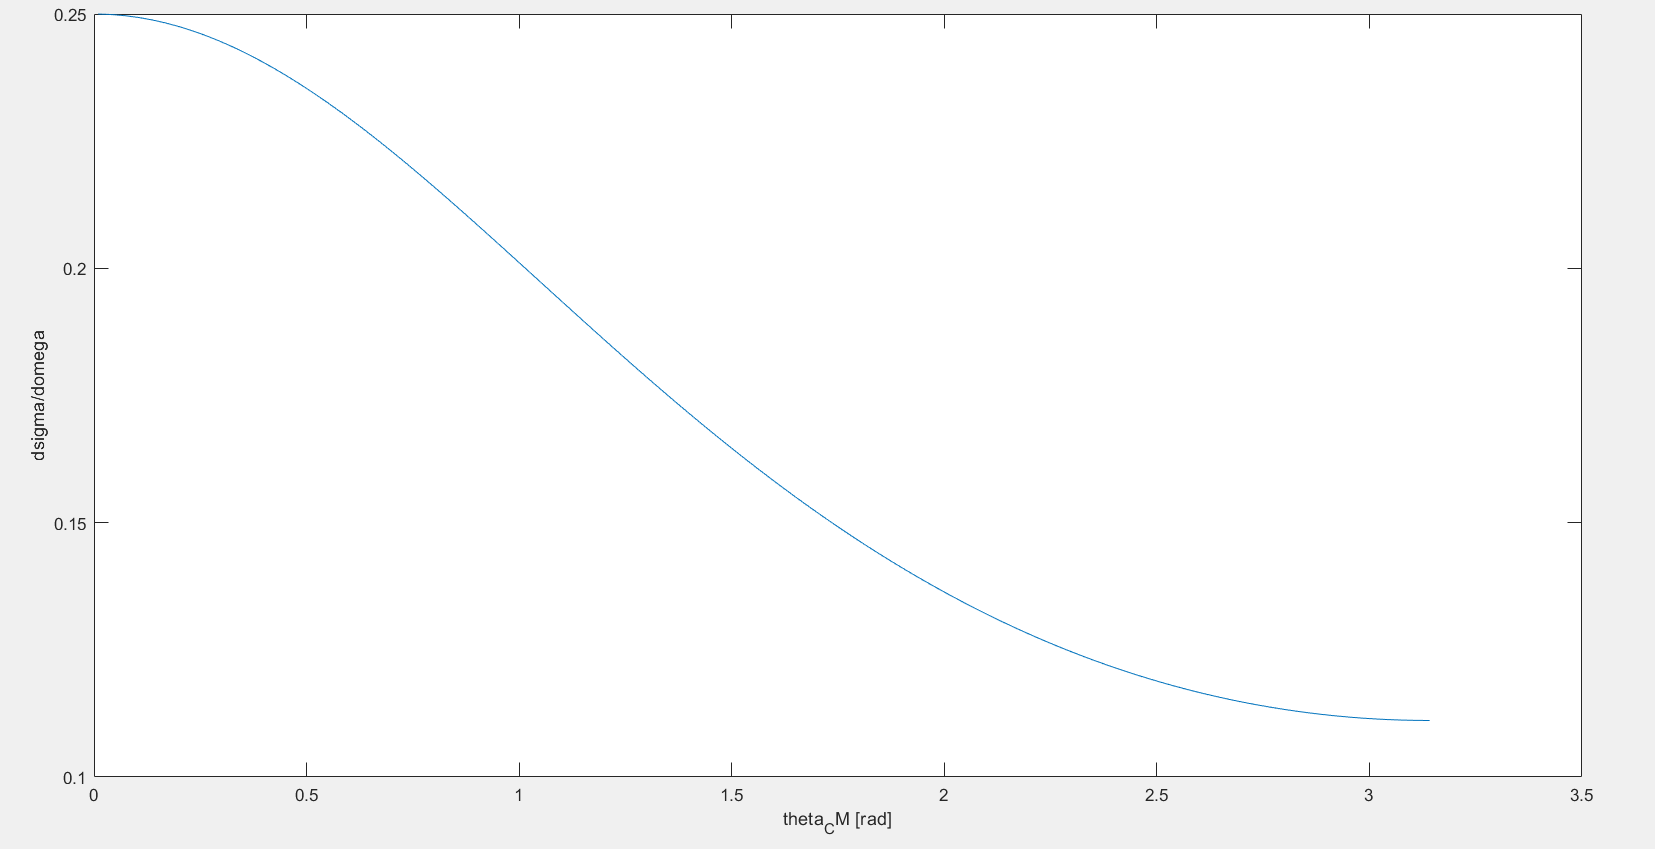
\includegraphics[scale = 0.3]{Images4/Diffusion2.PNG}
    \caption{Résultat théorique de la section efficace de Rutherford pour la diffusion neutron/proton}
    \label{sect_eff_diff_np_th}
\end{figure}


\subsection{Incohérence théorique et découverte des autres pions}


En réalité on observe pas la courbe en $\dfrac{1}{(\sin^2 + m^2)^2}$ de la figure \ref{sect_eff_diff_np_th} mais plutôt une forme comme sur la figure \ref{sect_eff_diff_np_exp} (le graphe expérimental est symétrique). Le graphe présente une remontée dans les grands angles. On remarque aussi (et ce n'est pas représenté que le graphe) que pour des plus grandes énergie incidente le graphe s'abaisse uniformément. C'est compréhensible car on peut facilement supposer que de plus grandes quantités de mouvement incidentes augmenteront la quantité de mouvement échangée $\Vec{q}$ et la dépendance de la section efficace est en $\dfrac{1}{m^2 + q^2}$.\\
Cependant, la remontée est à ce stade incompréhensible et semble mettre notre théorie en péril.\\
\begin{figure}[H]
    \centering
    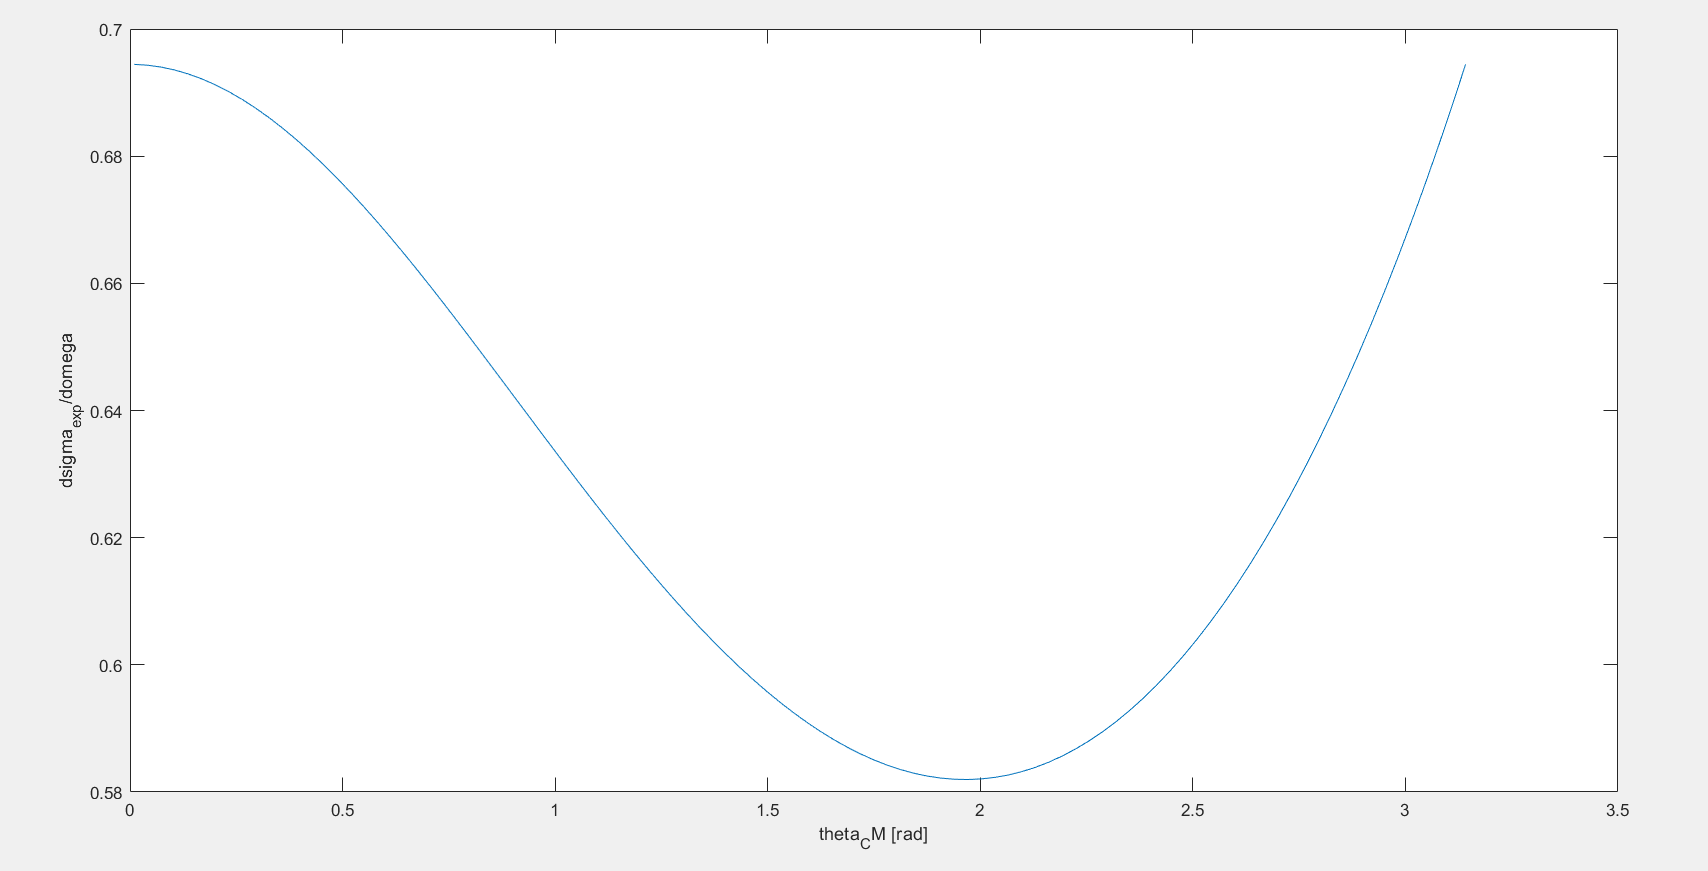
\includegraphics[scale = 0.3]{Images4/Diffusion3.PNG}
    \caption{Résultat expérimental de la section efficace de Rutherford pour la diffusion neutron/proton}
    \label{sect_eff_diff_np_exp}
\end{figure}
Cette remontée du graphe exprime un nombre important de diffusions à grand angle (la minimum de graphe se trouve à 90\degree). Pour expliquer ce phénomène, il nous faut accepter l'existence de pions de charge positive $\pi^+$ et négative $\pi^-$. On parle d'une particule d'isospin $I=1$, le pion $\pi$, qui a $2I +1 =3$ états de charge différents : $\pi^+,\pi^-,\pi^0$. Pour mieux comprendre ceci, représentons la diffusion dans les diagrammes de Feynman.
\begin{figure}[H]
    \centering
    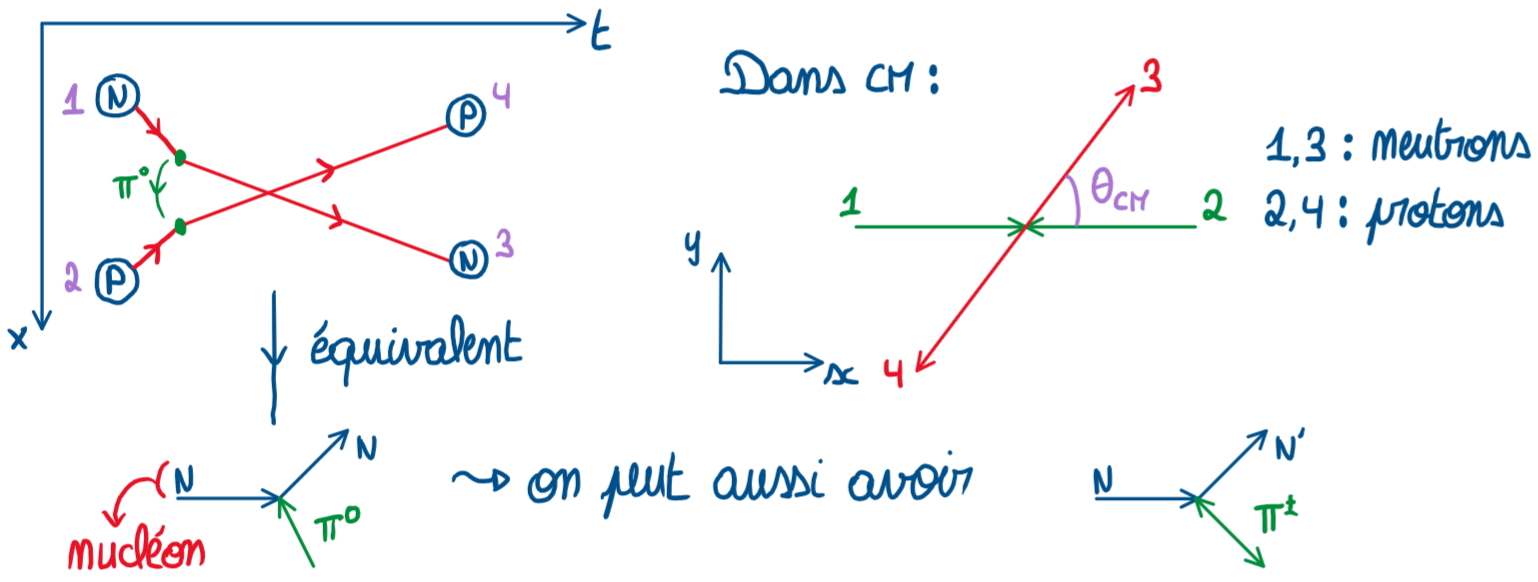
\includegraphics[scale = 0.5]{Images4/Feynmann_pi.png}
\end{figure}
On présente donc ici deux diagrammes différents, un dans l'espace-temps (Feynmann) et un x-y (habituel). Nous imposons les états asymptotiques (3:n,4:p). Cependant, il reste deux possibilités d'interaction : soit les particules demeurent les mêmes (c'est ce que représente le diagramme espace-temps de la figure ci-dessus) et sont simplement diffusées, soit les particules sont échangées (cfr. petit schéma en bas à droite) et diffusées à des angles différents.\\

Décrivons plus précisément le processus d'interaction : les particules s'approchent et à un moment quelconque, l'une émet un quanta d'échange, un méson et donc ici un pion. En émettant celui-ci la particule change sa trajectoire et éventuellement sa charge. La seconde particule reçoit ensuite le quanta et modifie à son tour sa trajectoire et éventuellement sa charge. On distingue donc les deux cas de figure : les particules sont inversées ou elles ne le sont pas. Dans le cas où elles ne sont pas inversées, il n'y a pas de transfert de charge, le méson échangé est donc un pion neutre $\pi^0$. Dans le cas où les particules sont inversées, le méson échangé est soit un $\pi^+$ soit un $\pi^-$. Comment sait-on laquelle est émise? Hé bien, on ne peut pas\footnote{Dans notre discussion, il est possible de le savoir mais la fonction d'onde s'effondrerait sur sa valeur propre. Ce qui revient à imposer au méson de passer par un trou en particulier, ce qui mène aux conséquences connues.} et on a pas besoin de le savoir, soit le proton émet un $\pi^+$ soit le neutron émet un $\pi^-$ le résultat est le même. En mécanique quantique, on somme toutes les possibilités interférentes amenant à une même situation finale et c'est exactement ce qu'on a ici ! En termes profanes, les deux phénomènes ont lieu en même temps : <<l'électron passe par les deux fentes>> !\\

Revenons maintenant à $q$, la quantité de mouvement échangée par les particules qui est simplement la quantité de mouvement de leur méson d'interaction. On comprend également en quoi notre calcul précédent était incorrect, nous n'avions considéré qu'une des deux possibilités interférentes, celles de l'interaction caractérisée par un pion neutre. Corrigeons donc notre erreur.\\
\begin{figure}[H]
    \centering
    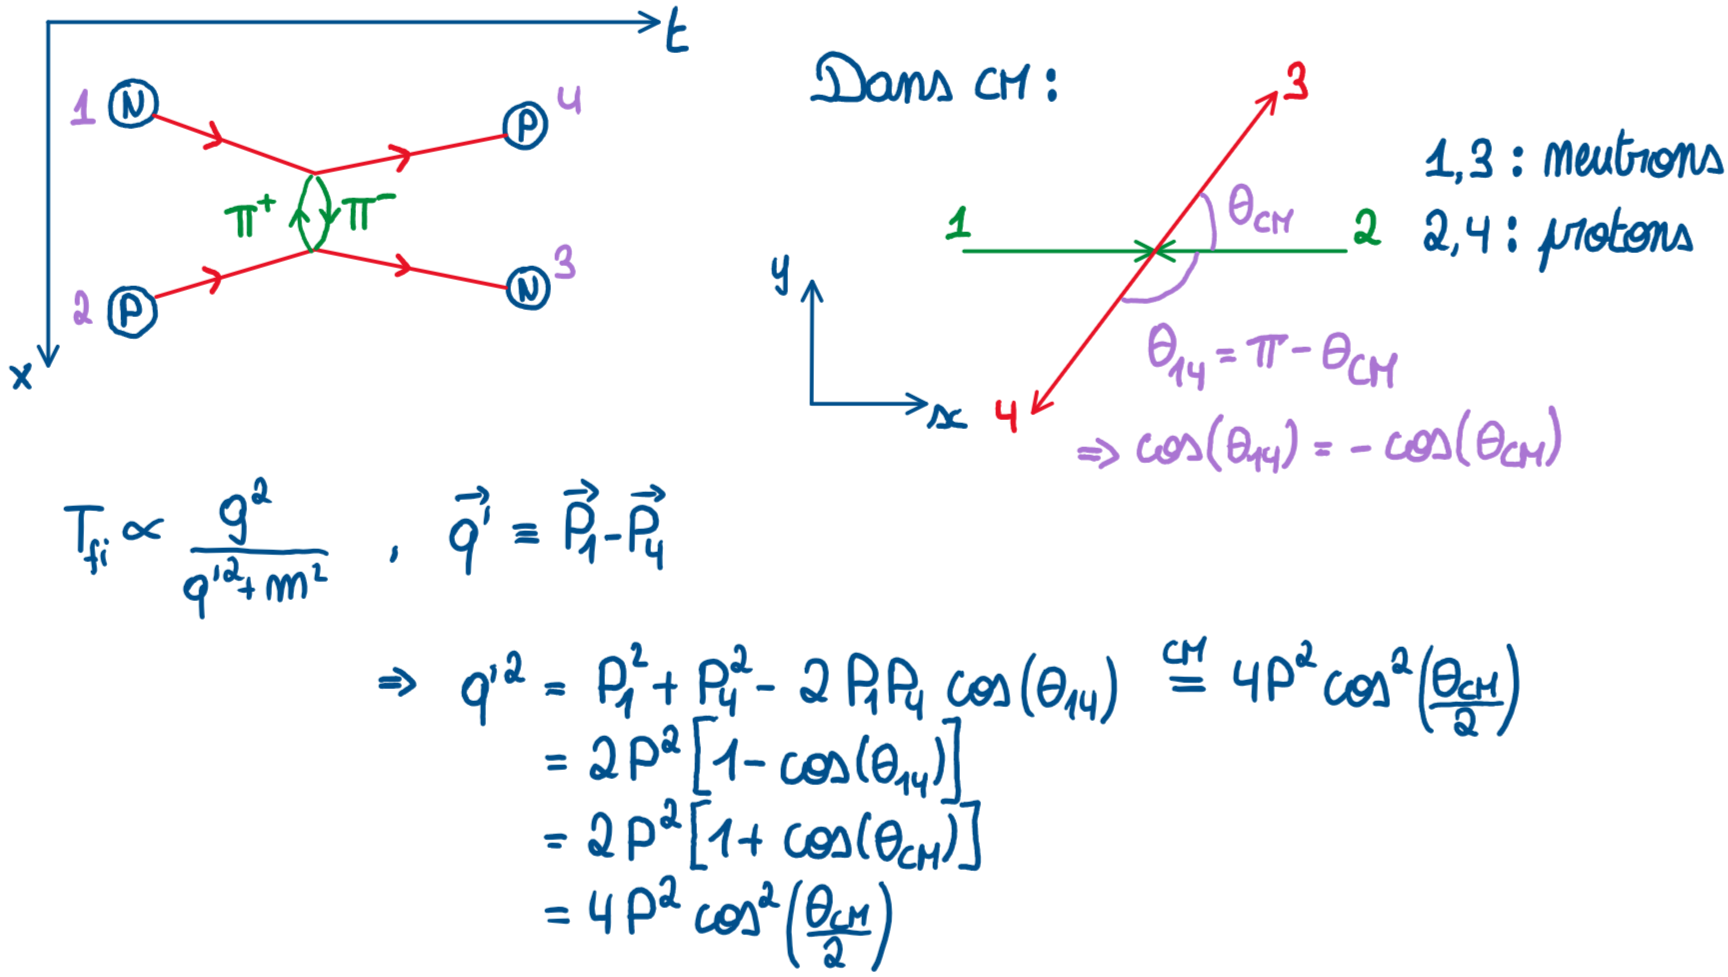
\includegraphics[scale = 0.4]{Images4/Feynmann_pi2.png}
\end{figure}
L'angle $\theta_{CM}$ est toujours l'angle entre le proton et le neutron seulement si nous considérons l'interaction qui fait intervenir les pions de charge non-nulle, il nous faut donc changer cet angle.
\[
    \theta_{14} \eq \pi - \theta_{CM}
\]
On obtient la même expression mais avec un cosinus ! Rien de compliqué donc. On obtient finalement pour la section efficace différentielle.
\[
    \boxed{
        T_{fi} \; \propto\; g^2 \left(\dfrac{1}{m_\pi^2 + q^2} + \dfrac{1}{m_\pi^2 + q'^2}\right)
    }
\]
\[
    \boxed{
        \fdif{\sigma}{\Omega}\Big|_{CM} \;\propto\;\alpha_s^2 \left(\dfrac{1}{2m_n T \sin^2(\dfrac{\theta_{CM}}{2})+m^2_\pi} + \dfrac{1}{2m_n T cos^2(\dfrac{\theta_{CM}}{2})+m^2_\pi}\right)^2
    }
\]
Le modèle de Yukawa est donc en opposition à ce que nous aurions pu attendre d'une expérience Rutherford. La proportion de neutrons rétrodiffusés est équivalente à celle des protons diffusés !
Remarques :
\begin{itemize}[label = $\bullet$]
    \item On retrouve bien la dépendance en l'inverse de l'énergie cinétique incidente $T$ pressentie plus tôt.
    \item Dans le référentiel du laboratoire, on écrit : $p_n = m_n v_n$. En réexprimant dans le référentiel centre de masse et en fonction de l'énergie cinétique :
    \begin{align*}
        P_{CM} & \eq P_1\\
        &\eq \dfrac{m_n v_n}{2}
        & \eq\dfrac{1}{2}\sqrt{2M T_\text{cin}}
    \end{align*}
    \[
        P^2 \eq \dfrac{1}{2}m_n T_\text{cin}^{labo}
    \]
    \item Dans notre modèle, nous avons supposé que la masse des pions $\pi^+,\pi^-,\pi^0$ était identique, ce qui n'est vrai qu'en première approximation.
\end{itemize}
Nous avons donc que, théoriquement et expérimentalement, on a autant de collision neutron/proton à grand angle ($\theta \rightarrow 180\degree$, rétrodiffusion) que que collision à petit angle ($\theta \rightarrow 0\degree$) 


\subsection{Observation des pions dans le rayonnement cosmique}


Par l'envoi de chambres à émulsion dans la haute atmosphère, on observe la décomposition des pions en muons. 
\[
    \pi^\pm \; \longrightarrow \; \mu^\pm +(\nu^{(-)}_e) + (\nu^{(-)}_e)\; \longrightarrow \; e^\pm  + (\nu_e^{(-)})  + (\nu_\mu^{(-)})
\]
On observe ainsi que le pion se désintègre quasiment à l'arrêt (la particule a un temps de vie plus long qu'un temps d'arrêt)   p et l'étude du \emph{range}, de la distance parcourue dans l'émulsion nous permet, connaissant la masse du muon par d'autres expériences, de déterminer la masse du pion.\\


\begin{figure}[H]
    \centering
    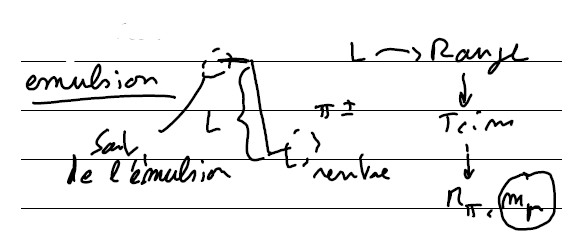
\includegraphics{Images4/masse_pion.PNG}
\end{figure}

On observe des traces dans les émulsions :
\begin{figure}[H]
    \centering
    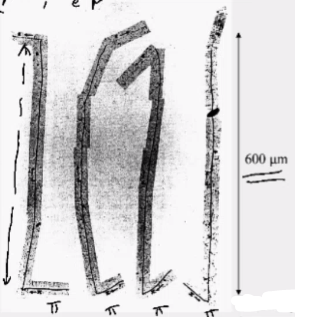
\includegraphics{Images4/traces.png}
\end{figure}
Les angles nous indiquent qu'il y a eu des processus de désintégration. La longueur du trait de $600\mu m$ est caractéristique. Par l'intégration de l'inverse de la formule de Bethe-Bloch on peut obtenir la distance parcourue par la particule.
\[
    D\eq \int \underbrace{\fdif{x}{E}}_{BB^{-1}} \dif E
\]
Par la cinématique de la désintégration du pion de masse $M$, on peut réécrire l'énergie du muon ($m_\mu$) émis car on connait sa masse. (En unités naturelles et en ignorant l'énergie cinétique du neutrino)
\[
    E_\mu \eq \dfrac{(M^2 + m_\mu^2)}{2M}\quad \text{avec} \; M \eq \SI{140}{MeV}; \; m_\mu \eq \SI{106}{MeV}
\]
\[
    E_\mu \eq T + m_\mu
\]
\[
    \rightarrow\;T\eq \SI{4.1}{MeV}
\]
\[
    \rightarrow \; D \; \approx \; 600\mu m \; <<< \; \tau_\mu c \eq 600m
\]
On voit donc bien que le muon a largement le temps de s'arrêter avant de se désintégrer. Il achève donc son temps de vie à l'arrêt à l'exception des diffusions avec les autres particules du milieu à cause de l'agitation thermique.\\

En conclusion, ces observations expérimentales ont fourni des preuves prématurées (tout ceci a eu lieu avant les expériences de collision forcée développées plus bas) de l'existence du pion. Pour les interpréter, il faut faire appel au pouvoir de pénétration des particules via la formule de Bethe-Bloch et à la distance parcourue pour en déduire l'énergie cinétique initiale du muon. Enfin, moyennant que l'on connaisse la masse du muon, on peut en déduire la désintégration qui l'a engendré ainsi que la masse de la particule associée, j'ai nommé : le pion.

\subsection{Découverte d'autres particules}


Le découverte de nombreuses autres particules ont suivi dans la foulée : $\underbrace{\rho}_{\SI{750}{MeV}}$, $\underbrace{\omega^{0,\pm},\eta, \sigma}_{1GeV}$ ...\\
Ces particules possédant une masse bien plus grande que la masse du pion, leur ordre était supérieur à celui de notre développement et donc leur participation négligeable. Cependant, pour de grandes valeurs d'énergie incidente et donc de $q$, on peut les observer. On découvre ainsi que $\omega^-$ est le méson à l'origine de la répulsion à très courte distance. On a donc un potentiel d'interaction qui devient la somme des interactions faisant intervenir chaque méson.\footnote{Dans l'expression qui suit, l'interaction avec $\omega$ est répulsive, il n'y a rien d'évident à cela mais cette notion dépasse largement le cadre du cours.}
\[
    V_{NN}\eq - \dfrac{g^2_\pi}{r}e^{-m_\pi r} +  \dfrac{g^2_\omega}{r}e^{-m_\omega r} +\ ...
\]
\begin{figure}[H]
    \centering
    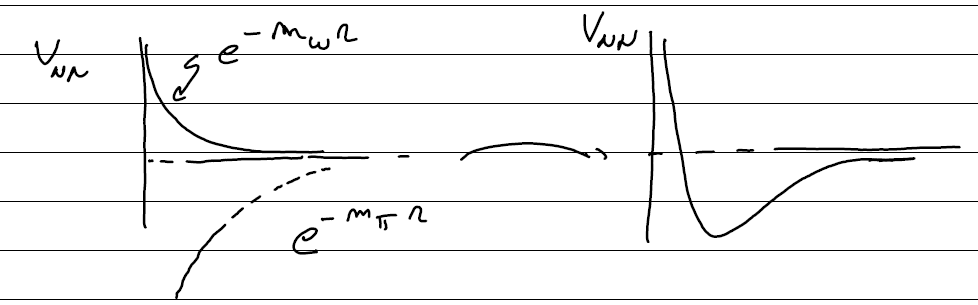
\includegraphics[scale = 0.8]{Images4/Potentiel NN.PNG}
\end{figure}
Cette petite illustration résume bien le succès de l'interprétation de Yukawa, via l'introduction de nouveaux objets, de nouvelles particules, on peut représenter des couplages inédits sensibles à toute une série de caractéristiques de nucléons tels que leurs spins, leurs moments angulaires etc... ou encore des produits combinés de ces valeurs. Cette approche phénoménologique est très appliquée et efficace en physique des particules.\\
Cependant, on aboutit à un nombre exorbitant de particules qu'il va nous falloir réduire à une série limitée d'interactions et de notion, mais il s'agit d'une autre histoire à base de quarks...
\subsection{Le potentiel moyen et la structure en couches}
A ce stade, nous avons pu mettre en évidence de façon grossière l'existence d'états liés nucléaires à l'aide du modèle très naïf du potentiel carré. Ce modèle ne permet pas d'expliquer l'existence de nombres magiques correspondant à des discontinuités dans l'énergie de liaison moyenne par nucléon.
\begin{figure}[H]
    \centering
    \includegraphics{Images4/BA_expé.PNG}
    \caption{}
\end{figure}
Ces nombres magiques sont le résultat de la saturation de couches de nucléons comme nous allons le voir tout de suite.
\subsubsection{Le modèle du gaz de Fermi}
Nous considérons simplement une ensemble de nucléons confinés dans un volume $V$ grâce à un potentiel moyen. Nous avions supposé un puits sphérique (forme carrée de potentiel en 1D). Le caractère fini de ce volume impose une quantification des états des nucléons. Ce qui signifie que pour calculer l'énergie de tous les nucléons enfermés dans cette boite on procède comme suit :
\[
    T_{tot} \eq \sum_i \dfrac{P_i^2}{2m}
\]
Les nucléons sont encore et toujours des fermions, nous devons donc satisfaire le principe d'exclusion. Pour obtenir l'état fondamental du système, il nous faut donc remplir tous les états possibles en partant des "plus bas". On est ici dans un cas exactement analogue à la sphère de Fermi des électrons de conduction dans un métal en physique de l'état solide. Les électrons se répartissent dans les états d'énergie en partant des plus bas et on retrouve donc dans l'espace 3D des nombres d'onde une boule dont la frontière est la sphère de rayon $k_F$. Dans le cas des nucléons, nous appellerons la quantité de mouvement frontière $q_F$ associée à l'énergie de Fermi $E_F$. Nous travaillons dans un cadre non-relativiste, on peut donc écrire pour ce potentiel :
\[
    E_F \eq \dfrac{P_F^2}{2m}
\]
Il nous faut maintenant nous pencher sur la densité d'états dans l'espace de $p$. Nous notons $\dif n$ le nombre d'états situés dans une portion de sphère indicée $\dif\Omega$ d'épaisseur $\dif p$. Nous notons également le volume minimal dans l'espace $p$ comme $\dfrac{(2\pi)^3}{\nu}$ où $\nu$ représente un volume matériel, ici le volume de confinement. Il nous faut ici introduire une approximation : bien que nous sachions que les états sont discrétisés, nous allons considérer que ceux-ci sont assez proches et nombreux pour passer à une forme intégrale (c'est une hypothèse hautement critiquable pour des systèmes $A<30$).
\[
    \dif n \eq \underbrace{(2I+1)(2S+1)}_{\text{mult. de spin et d'isospin}}\dfrac{p^2\dif p \dif \Omega}{\dfrac{(2\pi)^3}{\nu}}
\]
Comme dans le cas de la sphère de Fermi, intégrer la densité d'état sur la sphère doit redonner le nombre d'électrons de conduction. Nous intégrons donc sur notre sphère pour retrouver le nombre de nucléons $A$.
\[
    A\eq \int_S\int_0^{P_F} \fdif{n}{p}\dif p \dif \Omega
\]
On a une intégrale angulaire sur la surface de la sphère $\int_S \dif\Omega$ qui donne un terme $4\pi$ ainsi que l'intégrale de $p^2$. On se sert également de la relation entre $A$ et $r_0^3$
\[
    P_F c \eq \dfrac{\hbar c}{r_0}(\dfrac{9\pi}{8})^{\dfrac{1}{3}}\; \approx \; \SI{250}{MeV}
\]
\[
    E_F\eq \dfrac{P_F^2}{2m}  \; \approx \; \SI{35}{MeV}
\]
On calcule ensuite l'énergie totale du système en oubliant pas de normaliser.
\[
    T_{tot}\eq \int_0^{P_F} \dfrac{p^2}{2m}\dif n 
    \eq \dfrac{A}{2m} \dfrac{\int_0^{P_F} p^2 \fdif{n}{p}\dif p}{\int_0^{P_F}\dif n}
    \eq \dfrac{3}{5} A E_F
\]
Car on a que\footnote{Dans les notes de M.Lemaître, le tout est encore multiplié par $\nu$ mais il s'agit d'une erreur je pense.} :
\[
    A \eq \int_S\int_0^{P_F}\dif n \dif\Omega \eq \int_S\int_0^{P_F}\fdif{n}{p} \dif p \dif\Omega \eq \dfrac{4\nu}{(2\pi\hbar)^3} 4\pi \dfrac{P_F^3}{3}
\]
Nous venons d'obtenir la somme des énergies cinétiques. Pour estimer l'énergie potentielle du système, nous nous servons bien entendu de l'hypothèse du potentiel moyen. On peut représenter la situation comme suit :
\begin{figure}
    \centering
    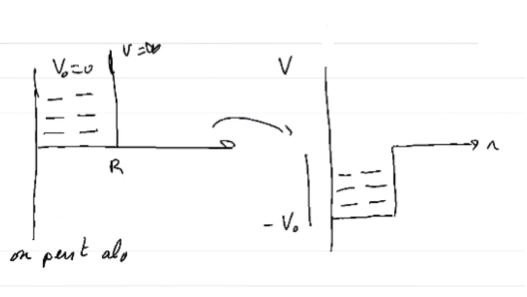
\includegraphics{Images4/puits2.PNG}
\end{figure}
On a tout simplement :
\[
    V_{tot} \eq -A V_0
\]
De par la courbe d'Aston, nous avons également la moyenne de l'énergie moyenne par nucléon.
\[
    \expval{B} \eq \dfrac{B}{A} \eq \SI{8}{MeV}
\]
\[
    -B \eq T_{tot} + V_{tot} \eq \dfrac{3}{5}A E_F - V_0 A
\]
On peut donc fournir une estimation de $V_0$.
\[
    V_0 \; \approx \; \SI{29}{MeV}
\]
\subsubsection{Prendre en compte le moment cinétique des nucléons}
Le développement sera similaire à ce qui a été fait pour le deuton à la différence que pour celui-ci on était toujours dans le cas de figure $l=0$ \footnote{Voir partie REF}. Pour continuer l'analogie avec la physique des solides, on a jusqu'ici considéré le cas d'électrons libres et on intègre maintenant un potentiel d'attraction moyen $V_0$.\\
On écrit l'équation de Schrödinger en coordonnées sphériques.
\[
       \dfrac{-\hbar^2}{2m} \left(\ffdif{\chi(r)}{r} + \dfrac{2}{r}\fdif{chi(r)}{r} - \dfrac{l(l+1)}{r^2}\right)\eq (E-V(r))\chi(r)
\]

\[
    V(r) \eq -V_0
\]

\[
    \boxed{
       \dfrac{-\hbar^2}{2m} \left(\ffdif{\chi(r)}{r} + \dfrac{2}{r}\fdif{chi(r)}{r} - \dfrac{l(l+1)}{r^2}\right)\eq (E+V_0)\chi(r)
    }
\]
où $m$ est la masse du nucléon.\\
Les solutions de ces équations sont connues : les fameuses fonctions de Bessel sphériques $J_l(r)$.
\paragraph{Pour $l=0$ :} on obtient facilement une solution en sinus cardinal sphérique qui correspond à notre solution de Bessel $J_0(r)$. Il faut ici être bien attentif à la définition de $J_0(r)$ ainsi qu'à la différence entre $A$ et $A'$, l'un contient $k_1$ l'autre non.
\begin{align*}
    \chi(r) &\eq A\dfrac{\sin(k_1r)}{r}\; \text{avec}\; k_1 \eq \sqrt{2m(E+V_0}\\
    &\eq A' \dfrac{\sin(k_1r)}{k_1 r}\\
    &\eq A'J_0(k_1 r)
\end{align*}
%Dans les notes de Lemaître, c'est un A et non un A' à la dernière ligne, c'est très probablement une erreur vu que J_0 correspond classiquement au simple sinus cardinal
Dans notre développement nous effectuons une énorme simplification : plutôt que de considérer la décroissance exponentielle dans la zone classiquement interdite et d'imposer la continuité de la fonction d'onde, nous imposons simplement son annulation à la fin du potentiel soir en $r = a$.
\[
    AJ_0(k_1a) \eq 0 \; \longrightarrow \; k_1 a \eq \pi,2\pi \ etc
\]
\paragraph{Pour l $\neq$ 0 :} Les fonctions de Bessel sphériques sont plus complexes mais toujours composées de fonctions trigonométriques divisées par des polynômes de $r$. Par exemple :
\[
    J_1(k_1 r) \eq \dfrac{\sin(k_1 r)}{(k_1 r)^2} - \dfrac{\cos(k_1r)}{k_1r}
\]
Les racines de la fonctions ne sont plus exprimables en multiples de $\pi$ mais l'idée demeure la même.
\[
    AJ_1(k_1a) \eq 0 \; \longrightarrow \; k_1 a \eq 4.49,7.73 \ etc
\]
On a toujours la relation analogue aux électrons libres :
\[
    E_{nl} \eq \dfrac{\hbar^2k_{nl}^2}{2m}
\]
$k$ dépend donc de $l$ et à travers lui $E$ également. En termes physiques l'effet centrifuge influe sur les niveaux d'énergie des nucléons. On peut également deviner que l'énergie sera indépendante de $m$ la projection du moment orbital sur un axe car le noyau présente une symétrie sphérique.\\
En multipliant les multiplicités de spin, d'isospin et de moment orbital, on peut obtenir la dégénérescence d'une valeur d'énergie.
\[
    \#etats \eq (2I+1)(2S+1)(2l+1)
\]
On a désormais tous les ingrédients pour construire une échelle des niveaux d'énergie en fonction des nombres quantiques des nucléons mais avant ça faisons un détour par la probabilité de présence radiale.\\
On note la probabilité de trouver la particule dans une coquille sphérique s'étendant sur$ [r,r+dr]$.
\[
    P(r)dr \eq |\chi(r)|^2 r^2 \dif r \underbrace{\int_S Y_l^m(\theta,\phi)\dif\Omega}_{= 1 \text{par prop.}}
\]
\begin{figure}[H]
    \centering
    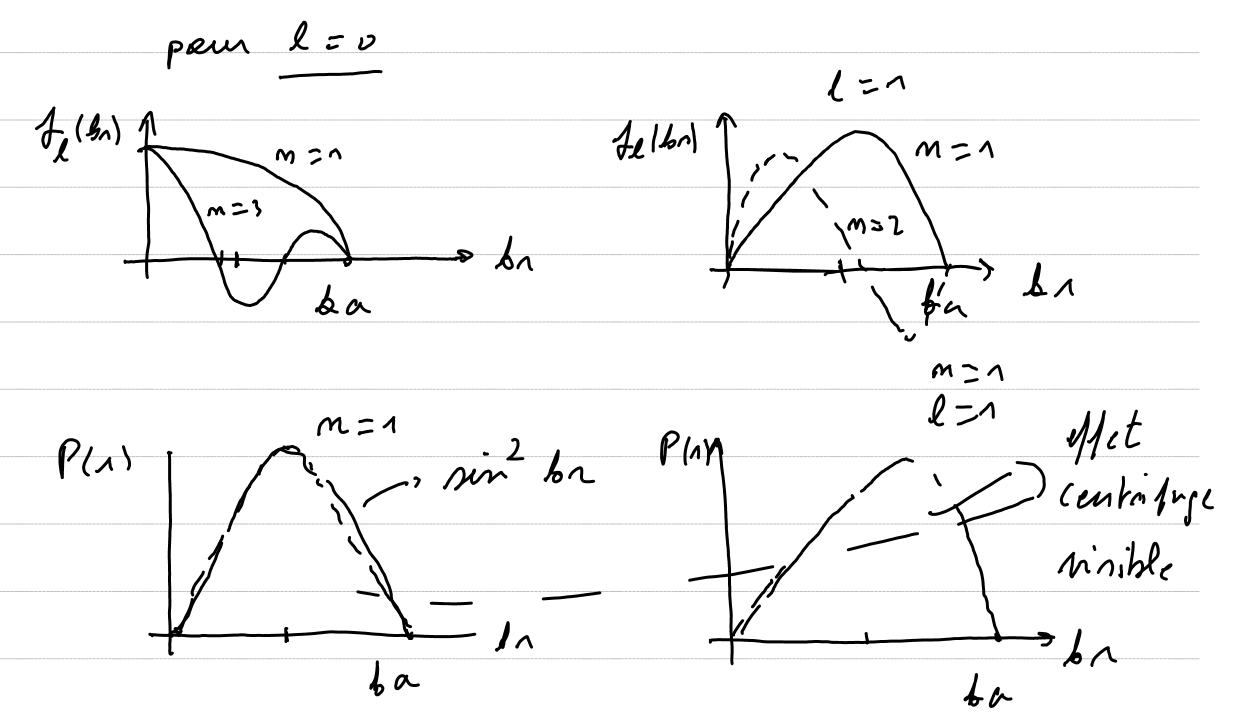
\includegraphics[scale = 0.6]{Images4/proba volumique.PNG}
    \caption{Sur la ligne du dessus, on a les densités de probabilité de présence, sur la ligne du dessous ce sont les probabilités radiales. Il semblerait qu'il y ait une erreur sur les deux graphes de droite : Il faut inverser n=1 et n=2 au-dessus et changer n=1 en n=2 en dessous.}
\end{figure}
On voit un comportement des fonctions d'onde assez analogue avec les fonctions d'onde des électrons dans l'atome d'hydrogène. Il est facile de déduire des nombres quantiques le nombre de noeuds de la fonction. On peut également en extraire un rayon le plus probable d'occupation, analogue au rayon de Bohr. On voit notamment que ce rayon de Borh est repoussé par les effets centrifuges quand $l = 1$.
\subsubsection{Comment modéliser en pratique ?}
Tout comme la méthode de Hartree-Fock, on aboutit à une expression implicite. En clair, le potentiel moyen dépend des fonctions d'onde et vice-versa. On part d'abord d'une hypothèse simplificatrice : le potentiel carré vu précédemment est approximé par une fonction delta en $r_0$ de profondeur $V_0$. Pour obtenir une valeur concrète sans passer par cette approximation, il faut partir d'une estimation et itérer jusqu'à convergence.
\begin{figure}[H]
    \centering
    \includegraphics[scale = 0.8]{Images4/delta_potentiel.PNG}
\end{figure}
On a pu obtenir $\rho(\Vec{r})$ par la mesure de la section efficace, le calcul du facteur de forme etc. On peut donc estimer le potentiel moyen $V_{m}$ par une fonction implicite. Elle n'est évidemment plus implicite si on a $\rho(\vec({r)}$.
\[
    V_m(\vec{r}) \eq \dfrac{\int \rho(\vec{r}')V(\vec{r}-\vec{r}')d\vec{r'}^3}{\int \rho(r)d\vec{r}^3}\eq \dfrac{\int \rho(\vec{r}')-v_0\delta(\vec{r'}-\vec{r})d\vec{r'}^3}{1}\eq -v_0 \rho(\vec{r})
\]
Comme on a placé notre delta de Dirac en 0 :
\[
    V_m \eq v_0 \rho(0) \; \approx \; \SI{26}{MeV}
\]
où $v_0$ est la densité de potentiel, $\rho(0) \approx 0.15nucleons/\si{fm^3}$.\\

\begin{figure}[H]
    \centering
    \includegraphics[scale = 0.7]{Images4/itération.PNG}
\end{figure}
\begin{figure}[H]
    \centering
    \includegraphics[scale = 1.2]{Images4/schéma_itération.PNG}
\end{figure}
\subsubsection{Modèles du puits infini et de l'oscillateur harmonique}
\begin{figure}[H]
    \centering
    \includegraphics[scale = 0.6]{Images4/infinite_well_and_harmonic_oscillator.PNG}
\end{figure}
Rappelons les nombres magiques identifiés sur le graphe de l'énergie moyenne de liaison par nucléon :
\[
    \boxed{
    \;A_m \eq [2,8,20,28,40,50,82,114,126]\;
    }
\]
Il est important de noter que les deux niveaux sont inversés par rapport à la physique atomique car le terme $g(r)$ est négatif.\\
On s'aperçoit donc que les deux modèles ne permettent de se rendre compte que des trois premiers nombres. Et c'est parce que nous avons ici omis une partie fondamentale de la physique de ces nucléons : l'interaction spin-orbite.\\
En effet, une des particularités de la physique nucléaire est l'importance prépondérante de cet effet pourtant relativiste en physique atomique.
\subsubsection{La correction spin-orbite}
On ajoute donc le terme spin-orbite au potentiel nucléon-nucléon de Wood-Saxon et on en profite pour ajouter l'interaction spin-spin nucléaire mais qui est largement moins importante.
\[
    V_{NN}\eq V_{WS}(r) 
    \; + \; \underbrace{\left(g(r)\vec{L}\cdot\vec{S}\right)}_\text{spin-orbite}
    \; + \; \underbrace{\left(f(r)\vec{\sigma}\cdot\vec{\sigma_n}\right)}_\text{spin-spin nucléaire}
\]
Le second terme, d'interaction spin-spin nucléaire, est important en pratique mais n'est pas abordé dans ce cours.\\
Explicitons d'abord ces interactions. La correction spin-spin correspond à l'interaction entre un nucléon et le spin du noyau. La correction spin-orbite correspond à l'interaction entre le spin du nucléon libre et le moment magnétique orbital total. Regardons à l'interaction spin-orbite.\\
On rappelle l'expression classique du moment magnétique total $\vec{J} :$
\[
    \vec{J} \eq \vec{L} + \vec{S}
\]
\[
    \Rightarrow \vec{L}\cdot\vec{S} \eq \dfrac{1}{2} \left(J^2 - L^2 - S^2\right)
\]
En physique nucléaire et contrairement à la physique atomique, nous avons $g(r) < 0$. l'interaction spin-orbite est donc liante.\\
\begin{figure}
    \centering
    \includegraphics[scale = 0.7]{Images4/spin-orbite_dégén.PNG}
    \caption{ATTENTION : l'expression correcte pour $\Delta E_-$ est : $l^2 + l +\dfrac{3}{4}$}
\end{figure}
On en tire donc l'expression en fonction de $l$ de l'écart en énergie entre les deux niveaux précédemment dégénérés.
\[
\boxed{
    \;\Delta E \eq -\expval{g}(l+\dfrac{1}{2})\;
    }
\]
Dans un modèle naïf, on peut supposer $g(r) = g_0$.
Il y a cependant ici une zone de flou : si en physique atomique il est aisé de définir une surface représentant le parcours de l'électron et donc d'en tirer le moment magnétique perpendiculaire généré, dans un noyau il n'y a pas de référentiel évident par rapport auquel définir l'orbite. Il nous faut donc ruser. En définissant un volume de confinement\footnote{C'est dans le thème en ce moment} pour la charge nucléaire, nous pouvons définir un centre de masse et donc avoir un point de référence pour définir notre orbite. La seule direction privilégiée dans un noyau sphérique est la direction radiale.
%J'ai pas du tout compris et le prof n'a pas vraiment expliqué cette histoire de nucléon libre, je suppose que c'est pcq le spin des couches fermées ne participe pas mais comment ça se fait que la correction modifie quand même des couches fermées alors?
\[
    L \; \propto\; \vec{r}\cross \vec{p}
\]
Comme nous savons que notre noyau respecte la symétrie sphérique par la mesure de la surface efficace, nous pouvons supposer que le couplage sera proportionnel au gradient de la densité de charge selon r.
\[
    \nabla \rho(\vec{r}) \eq \fdif{\rho}{r}\dfrac{\vec{r}}{r}
\]
\[
    \vec{r} \; \propto \; \nabla \rho(\vec{r})
\]
\[
    \vec{L}\;\propto\; \nabla \rho(\vec{r})\cross \vec{P}
\]
\[
    V_{SO}(r) \; \propto \; \left(\nabla \rho(\vec{r})\cross \vec{P}\right)\cdot \vec{S}
\]
\[
    V_{SO}(r) \eq\underbrace{  \lambda\fdif{\rho(r)}{r}\dfrac{1}{r}}_{= g(r)}\left(\vec{L}\cdot \vec{S}\right)
\]
\[
    g(r) \;\propto\; \dfrac{\partial V(r)}{\partial r} \; \text{car}\; \rho(r) \propto V(r)
\]
\begin{figure}[H]
    \centering
    \includegraphics{Images4/facteur_gamma.PNG}
\end{figure}
Sans surprise, cette correction lève la dégénérescence des niveaux des modèles précédents (puits infini et oscillateur harmonique). Revenons sur la notion d'état particulièrement stable. De façon tout à fait évidente, si le gap d'énergie au-dessus d'un état est particulièrement élevé, il sera particulièrement difficile de l'exciter et l'état sera donc dit stable. En levant la dégénérescence de ces niveaux, la correction spin-orbite va modifier l'écart entre les niveaux et donc modifier ceux dits stables. La correction étant particulièrement importante, elle va largement changer les nombres magiques caractérisant ces états.
\begin{figure}[H]
    \centering
    \includegraphics[width=\textwidth]{Images4/spin-orbite.PNG}
\end{figure}
\subsubsection{Noyaux pair-impair}
Le modèle marche également de façon tout à fait satisfaisante pour les noyaux pair-impair. Le nucléon non-apparié fait varier $\vec{J}$ et les corrections suivent.
\begin{figure}[H]
    \centering
    \includegraphics[width=\textwidth]{Images4/pair-impair.PNG}
\end{figure}






\section{Hypothèse subjective sur les théories physiques}
\emph{La discussion rapportée ici concerne la structure des théories physiques et de possibles futurs développements de celles-ci. Il ne s'agit pas à proprement parler de matière d'examen.}\\
On peut caractériser une théorie physique par deux choses :
\begin{itemize}[label = $\bullet$]
    \item \textbf{Les paramètres libres adimensionnels} représentent une série de valeurs invariantes d'échelle. Nous savons désormais que l'Univers est en expansion et l'adimensionnalité garantit une continuité dans le temps de nos théories physiques. Un exemple de paramètres libres sont les nombreuses particules auxquelles nous avons abouti à la fin de la discussion concernant l'hypothèse de Yukawa. Une théorie trop fournie en paramètres libres est flexible (on peut les régler pour satifsaire beaucoup d'expériences) mais est également symptomatique d'une interaction plus fondamentale permettant de regrouper tous ces phénomènes sous un nombre plus limités de bannières. Exemple : les particules de Yukawa sont en réalité constituées de quarks, gluons etc donc de particules <<fondamentales>>, leur nombre est plus limité et permet de rendre compte des effets de ces particules composites : pion, muon etc.
    \item \textbf{Les observables physiques} représentent des grandeurs mesurables absolues, dimensionelles et physiques (donc pas un nombre d'événements par seconde comme pour un courant par exemple), il en existe plusieurs jeux en compétition. Ces jeux sont toujours composés de 3 grandeurs qui permettent de recomposer le temps, la masse et la distance. Actuellement, il est admis que $h$ et $c$ devront être incluses car elles sont incluses dans toutes les théories et sont universelles. Pour la troisième, il y a une série de candidats : $k_B$, $M_{Planck}$, $M_{nucleon}$, $\Lambda$. Elle doit également être indépendante de toute théorie.
\end{itemize}
On a actuellement repéré une série de constantes permettant de définir les différentes théories physiques.
\begin{table}[H]
    \centering
    \begin{tabular}{|c|c|c|c|c|c|}
    \hline
         Interaction &em&forte&grav.&faible & Higgs  \\
         \hline
         Constante associée& $\alpha=\dfrac{e^2}{4\pi\epsilon_0\hbar c}$&$\alpha_s=\dfrac{g^2}{4\pi}$&$\dfrac{Gm_N}{\hbar^3}$&$\alpha$&???\\
         \hline
    \end{tabular}
\end{table}
Le fait que la constante $\alpha$ apparaisse dans les théories électromagnétiques et d'interaction faible est incroyable et indique que nous sommes sur la bonne voie pour l'unification des interactions. Il y a également des similitudes entre l'interaction de Higgs et l'interaction faible.